
\documentclass[11pt,letterpaper,english]{article}
\pdfoutput=1

\usepackage{bm}
\usepackage[margin=1in]{geometry}

\usepackage{microtype}
\usepackage{graphicx}
\usepackage{float}
\usepackage{caption}
\usepackage{subcaption}
\usepackage{booktabs} %
\usepackage{authblk}


\newcommand{\theHalgorithm}{\arabic{algorithm}}

\usepackage{natbib}


\usepackage{amsmath}
\usepackage{amssymb}
\usepackage{mathtools}
\usepackage{amsthm}

\theoremstyle{plain}
\newtheorem{theorem}{Theorem}[section]
\newtheorem{proposition}[theorem]{Proposition}
\newtheorem{lemma}[theorem]{Lemma}
\newtheorem{corollary}[theorem]{Corollary}
\theoremstyle{definition}
\newtheorem{definition}[theorem]{Definition}
\newtheorem{assumption}[theorem]{Assumption}
\theoremstyle{remark}
\newtheorem{remark}[theorem]{Remark}

\usepackage[disable]{todonotes}

\usepackage[pdfencoding=auto]{hyperref}

\usepackage[capitalize,noabbrev]{cleveref}
\usepackage{bookmark}

\hypersetup{pdfauthor={Ayoub Belhadji, Daniel Sharp, Youssef Marzouk},pdftitle={Weighted quantization using MMD: From mean field to mean shift via gradient flows}}


%
\setlength\unitlength{1mm}
\newcommand{\twodots}{\mathinner {\ldotp \ldotp}}
% bb font symbols
\newcommand{\Rho}{\mathrm{P}}
\newcommand{\Tau}{\mathrm{T}}

\newfont{\bbb}{msbm10 scaled 700}
\newcommand{\CCC}{\mbox{\bbb C}}

\newfont{\bb}{msbm10 scaled 1100}
\newcommand{\CC}{\mbox{\bb C}}
\newcommand{\PP}{\mbox{\bb P}}
\newcommand{\RR}{\mbox{\bb R}}
\newcommand{\QQ}{\mbox{\bb Q}}
\newcommand{\ZZ}{\mbox{\bb Z}}
\newcommand{\FF}{\mbox{\bb F}}
\newcommand{\GG}{\mbox{\bb G}}
\newcommand{\EE}{\mbox{\bb E}}
\newcommand{\NN}{\mbox{\bb N}}
\newcommand{\KK}{\mbox{\bb K}}
\newcommand{\HH}{\mbox{\bb H}}
\newcommand{\SSS}{\mbox{\bb S}}
\newcommand{\UU}{\mbox{\bb U}}
\newcommand{\VV}{\mbox{\bb V}}


\newcommand{\yy}{\mathbbm{y}}
\newcommand{\xx}{\mathbbm{x}}
\newcommand{\zz}{\mathbbm{z}}
\newcommand{\sss}{\mathbbm{s}}
\newcommand{\rr}{\mathbbm{r}}
\newcommand{\pp}{\mathbbm{p}}
\newcommand{\qq}{\mathbbm{q}}
\newcommand{\ww}{\mathbbm{w}}
\newcommand{\hh}{\mathbbm{h}}
\newcommand{\vvv}{\mathbbm{v}}

% Vectors

\newcommand{\av}{{\bf a}}
\newcommand{\bv}{{\bf b}}
\newcommand{\cv}{{\bf c}}
\newcommand{\dv}{{\bf d}}
\newcommand{\ev}{{\bf e}}
\newcommand{\fv}{{\bf f}}
\newcommand{\gv}{{\bf g}}
\newcommand{\hv}{{\bf h}}
\newcommand{\iv}{{\bf i}}
\newcommand{\jv}{{\bf j}}
\newcommand{\kv}{{\bf k}}
\newcommand{\lv}{{\bf l}}
\newcommand{\mv}{{\bf m}}
\newcommand{\nv}{{\bf n}}
\newcommand{\ov}{{\bf o}}
\newcommand{\pv}{{\bf p}}
\newcommand{\qv}{{\bf q}}
\newcommand{\rv}{{\bf r}}
\newcommand{\sv}{{\bf s}}
\newcommand{\tv}{{\bf t}}
\newcommand{\uv}{{\bf u}}
\newcommand{\wv}{{\bf w}}
\newcommand{\vv}{{\bf v}}
\newcommand{\xv}{{\bf x}}
\newcommand{\yv}{{\bf y}}
\newcommand{\zv}{{\bf z}}
\newcommand{\zerov}{{\bf 0}}
\newcommand{\onev}{{\bf 1}}

% Matrices

\newcommand{\Am}{{\bf A}}
\newcommand{\Bm}{{\bf B}}
\newcommand{\Cm}{{\bf C}}
\newcommand{\Dm}{{\bf D}}
\newcommand{\Em}{{\bf E}}
\newcommand{\Fm}{{\bf F}}
\newcommand{\Gm}{{\bf G}}
\newcommand{\Hm}{{\bf H}}
\newcommand{\Id}{{\bf I}}
\newcommand{\Jm}{{\bf J}}
\newcommand{\Km}{{\bf K}}
\newcommand{\Lm}{{\bf L}}
\newcommand{\Mm}{{\bf M}}
\newcommand{\Nm}{{\bf N}}
\newcommand{\Om}{{\bf O}}
\newcommand{\Pm}{{\bf P}}
\newcommand{\Qm}{{\bf Q}}
\newcommand{\Rm}{{\bf R}}
\newcommand{\Sm}{{\bf S}}
\newcommand{\Tm}{{\bf T}}
\newcommand{\Um}{{\bf U}}
\newcommand{\Wm}{{\bf W}}
\newcommand{\Vm}{{\bf V}}
\newcommand{\Xm}{{\bf X}}
\newcommand{\Ym}{{\bf Y}}
\newcommand{\Zm}{{\bf Z}}

% Calligraphic

\newcommand{\Ac}{{\cal A}}
\newcommand{\Bc}{{\cal B}}
\newcommand{\Cc}{{\cal C}}
\newcommand{\Dc}{{\cal D}}
\newcommand{\Ec}{{\cal E}}
\newcommand{\Fc}{{\cal F}}
\newcommand{\Gc}{{\cal G}}
\newcommand{\Hc}{{\cal H}}
\newcommand{\Ic}{{\cal I}}
\newcommand{\Jc}{{\cal J}}
\newcommand{\Kc}{{\cal K}}
\newcommand{\Lc}{{\cal L}}
\newcommand{\Mc}{{\cal M}}
\newcommand{\Nc}{{\cal N}}
\newcommand{\nc}{{\cal n}}
\newcommand{\Oc}{{\cal O}}
\newcommand{\Pc}{{\cal P}}
\newcommand{\Qc}{{\cal Q}}
\newcommand{\Rc}{{\cal R}}
\newcommand{\Sc}{{\cal S}}
\newcommand{\Tc}{{\cal T}}
\newcommand{\Uc}{{\cal U}}
\newcommand{\Wc}{{\cal W}}
\newcommand{\Vc}{{\cal V}}
\newcommand{\Xc}{{\cal X}}
\newcommand{\Yc}{{\cal Y}}
\newcommand{\Zc}{{\cal Z}}

% Bold greek letters

\newcommand{\alphav}{\hbox{\boldmath$\alpha$}}
\newcommand{\betav}{\hbox{\boldmath$\beta$}}
\newcommand{\gammav}{\hbox{\boldmath$\gamma$}}
\newcommand{\deltav}{\hbox{\boldmath$\delta$}}
\newcommand{\etav}{\hbox{\boldmath$\eta$}}
\newcommand{\lambdav}{\hbox{\boldmath$\lambda$}}
\newcommand{\epsilonv}{\hbox{\boldmath$\epsilon$}}
\newcommand{\nuv}{\hbox{\boldmath$\nu$}}
\newcommand{\muv}{\hbox{\boldmath$\mu$}}
\newcommand{\zetav}{\hbox{\boldmath$\zeta$}}
\newcommand{\phiv}{\hbox{\boldmath$\phi$}}
\newcommand{\psiv}{\hbox{\boldmath$\psi$}}
\newcommand{\thetav}{\hbox{\boldmath$\theta$}}
\newcommand{\tauv}{\hbox{\boldmath$\tau$}}
\newcommand{\omegav}{\hbox{\boldmath$\omega$}}
\newcommand{\xiv}{\hbox{\boldmath$\xi$}}
\newcommand{\sigmav}{\hbox{\boldmath$\sigma$}}
\newcommand{\piv}{\hbox{\boldmath$\pi$}}
\newcommand{\rhov}{\hbox{\boldmath$\rho$}}
\newcommand{\upsilonv}{\hbox{\boldmath$\upsilon$}}

\newcommand{\Gammam}{\hbox{\boldmath$\Gamma$}}
\newcommand{\Lambdam}{\hbox{\boldmath$\Lambda$}}
\newcommand{\Deltam}{\hbox{\boldmath$\Delta$}}
\newcommand{\Sigmam}{\hbox{\boldmath$\Sigma$}}
\newcommand{\Phim}{\hbox{\boldmath$\Phi$}}
\newcommand{\Pim}{\hbox{\boldmath$\Pi$}}
\newcommand{\Psim}{\hbox{\boldmath$\Psi$}}
\newcommand{\Thetam}{\hbox{\boldmath$\Theta$}}
\newcommand{\Omegam}{\hbox{\boldmath$\Omega$}}
\newcommand{\Xim}{\hbox{\boldmath$\Xi$}}


% Sans Serif small case

\newcommand{\Gsf}{{\sf G}}

\newcommand{\asf}{{\sf a}}
\newcommand{\bsf}{{\sf b}}
\newcommand{\csf}{{\sf c}}
\newcommand{\dsf}{{\sf d}}
\newcommand{\esf}{{\sf e}}
\newcommand{\fsf}{{\sf f}}
\newcommand{\gsf}{{\sf g}}
\newcommand{\hsf}{{\sf h}}
\newcommand{\isf}{{\sf i}}
\newcommand{\jsf}{{\sf j}}
\newcommand{\ksf}{{\sf k}}
\newcommand{\lsf}{{\sf l}}
\newcommand{\msf}{{\sf m}}
\newcommand{\nsf}{{\sf n}}
\newcommand{\osf}{{\sf o}}
\newcommand{\psf}{{\sf p}}
\newcommand{\qsf}{{\sf q}}
\newcommand{\rsf}{{\sf r}}
\newcommand{\ssf}{{\sf s}}
\newcommand{\tsf}{{\sf t}}
\newcommand{\usf}{{\sf u}}
\newcommand{\wsf}{{\sf w}}
\newcommand{\vsf}{{\sf v}}
\newcommand{\xsf}{{\sf x}}
\newcommand{\ysf}{{\sf y}}
\newcommand{\zsf}{{\sf z}}


% mixed symbols

\newcommand{\sinc}{{\hbox{sinc}}}
\newcommand{\diag}{{\hbox{diag}}}
\renewcommand{\det}{{\hbox{det}}}
\newcommand{\trace}{{\hbox{tr}}}
\newcommand{\sign}{{\hbox{sign}}}
\renewcommand{\arg}{{\hbox{arg}}}
\newcommand{\var}{{\hbox{var}}}
\newcommand{\cov}{{\hbox{cov}}}
\newcommand{\Ei}{{\rm E}_{\rm i}}
\renewcommand{\Re}{{\rm Re}}
\renewcommand{\Im}{{\rm Im}}
\newcommand{\eqdef}{\stackrel{\Delta}{=}}
\newcommand{\defines}{{\,\,\stackrel{\scriptscriptstyle \bigtriangleup}{=}\,\,}}
\newcommand{\<}{\left\langle}
\renewcommand{\>}{\right\rangle}
\newcommand{\herm}{{\sf H}}
\newcommand{\trasp}{{\sf T}}
\newcommand{\transp}{{\sf T}}
\renewcommand{\vec}{{\rm vec}}
\newcommand{\Psf}{{\sf P}}
\newcommand{\SINR}{{\sf SINR}}
\newcommand{\SNR}{{\sf SNR}}
\newcommand{\MMSE}{{\sf MMSE}}
\newcommand{\REF}{{\RED [REF]}}

% Markov chain
\usepackage{stmaryrd} % for \mkv 
\newcommand{\mkv}{-\!\!\!\!\minuso\!\!\!\!-}

% Colors

\newcommand{\RED}{\color[rgb]{1.00,0.10,0.10}}
\newcommand{\BLUE}{\color[rgb]{0,0,0.90}}
\newcommand{\GREEN}{\color[rgb]{0,0.80,0.20}}

%%%%%%%%%%%%%%%%%%%%%%%%%%%%%%%%%%%%%%%%%%
\usepackage{hyperref}
\hypersetup{
    bookmarks=true,         % show bookmarks bar?
    unicode=false,          % non-Latin characters in AcrobatÕs bookmarks
    pdftoolbar=true,        % show AcrobatÕs toolbar?
    pdfmenubar=true,        % show AcrobatÕs menu?
    pdffitwindow=false,     % window fit to page when opened
    pdfstartview={FitH},    % fits the width of the page to the window
%    pdftitle={My title},    % title
%    pdfauthor={Author},     % author
%    pdfsubject={Subject},   % subject of the document
%    pdfcreator={Creator},   % creator of the document
%    pdfproducer={Producer}, % producer of the document
%    pdfkeywords={keyword1} {key2} {key3}, % list of keywords
    pdfnewwindow=true,      % links in new window
    colorlinks=true,       % false: boxed links; true: colored links
    linkcolor=red,          % color of internal links (change box color with linkbordercolor)
    citecolor=green,        % color of links to bibliography
    filecolor=blue,      % color of file links
    urlcolor=blue           % color of external links
}
%%%%%%%%%%%%%%%%%%%%%%%%%%%%%%%%%%%%%%%%%%%



\newcommand\nnfootnote[1]{%
  \begin{NoHyper}
  \renewcommand\thefootnote{}\footnote{#1}%
  \addtocounter{footnote}{-1}%
  \end{NoHyper}
}

\begin{document}

\title{Weighted quantization using MMD:\\ From mean field to mean shift via gradient flows}


\author{Ayoub Belhadji\textsuperscript{*}}
\author{Daniel Sharp\textsuperscript{*}}
\author{Youssef Marzouk}

\affil{Center for Computational Science and Engineering\\ Massachusetts Institute of Technology}

\renewcommand{\Authands}{, }








\maketitle












{
\makeatletter\def\Hy@Warning#1{}\makeatother
\renewcommand{\thefootnote}{}
\footnotetext{*Equal contributions. Author emails: \href{mailto:abelhadj@mit.edu}{abelhadj@mit.edu}, \href{mailto:dannys4@mit.edu}{dannys4@mit.edu}, \href{mailto:ymarz@mit.edu}{ymarz@mit.edu}}
\renewcommand{\thefootnote}{0}
}

\begin{abstract}
\begin{abstract}  
Test time scaling is currently one of the most active research areas that shows promise after training time scaling has reached its limits.
Deep-thinking (DT) models are a class of recurrent models that can perform easy-to-hard generalization by assigning more compute to harder test samples.
However, due to their inability to determine the complexity of a test sample, DT models have to use a large amount of computation for both easy and hard test samples.
Excessive test time computation is wasteful and can cause the ``overthinking'' problem where more test time computation leads to worse results.
In this paper, we introduce a test time training method for determining the optimal amount of computation needed for each sample during test time.
We also propose Conv-LiGRU, a novel recurrent architecture for efficient and robust visual reasoning. 
Extensive experiments demonstrate that Conv-LiGRU is more stable than DT, effectively mitigates the ``overthinking'' phenomenon, and achieves superior accuracy.
\end{abstract}  











\end{abstract}

\section{Introduction}\label{sec:intro}
\section{Introduction}
\label{sec:introduction}
The business processes of organizations are experiencing ever-increasing complexity due to the large amount of data, high number of users, and high-tech devices involved \cite{martin2021pmopportunitieschallenges, beerepoot2023biggestbpmproblems}. This complexity may cause business processes to deviate from normal control flow due to unforeseen and disruptive anomalies \cite{adams2023proceddsriftdetection}. These control-flow anomalies manifest as unknown, skipped, and wrongly-ordered activities in the traces of event logs monitored from the execution of business processes \cite{ko2023adsystematicreview}. For the sake of clarity, let us consider an illustrative example of such anomalies. Figure \ref{FP_ANOMALIES} shows a so-called event log footprint, which captures the control flow relations of four activities of a hypothetical event log. In particular, this footprint captures the control-flow relations between activities \texttt{a}, \texttt{b}, \texttt{c} and \texttt{d}. These are the causal ($\rightarrow$) relation, concurrent ($\parallel$) relation, and other ($\#$) relations such as exclusivity or non-local dependency \cite{aalst2022pmhandbook}. In addition, on the right are six traces, of which five exhibit skipped, wrongly-ordered and unknown control-flow anomalies. For example, $\langle$\texttt{a b d}$\rangle$ has a skipped activity, which is \texttt{c}. Because of this skipped activity, the control-flow relation \texttt{b}$\,\#\,$\texttt{d} is violated, since \texttt{d} directly follows \texttt{b} in the anomalous trace.
\begin{figure}[!t]
\centering
\includegraphics[width=0.9\columnwidth]{images/FP_ANOMALIES.png}
\caption{An example event log footprint with six traces, of which five exhibit control-flow anomalies.}
\label{FP_ANOMALIES}
\end{figure}

\subsection{Control-flow anomaly detection}
Control-flow anomaly detection techniques aim to characterize the normal control flow from event logs and verify whether these deviations occur in new event logs \cite{ko2023adsystematicreview}. To develop control-flow anomaly detection techniques, \revision{process mining} has seen widespread adoption owing to process discovery and \revision{conformance checking}. On the one hand, process discovery is a set of algorithms that encode control-flow relations as a set of model elements and constraints according to a given modeling formalism \cite{aalst2022pmhandbook}; hereafter, we refer to the Petri net, a widespread modeling formalism. On the other hand, \revision{conformance checking} is an explainable set of algorithms that allows linking any deviations with the reference Petri net and providing the fitness measure, namely a measure of how much the Petri net fits the new event log \cite{aalst2022pmhandbook}. Many control-flow anomaly detection techniques based on \revision{conformance checking} (hereafter, \revision{conformance checking}-based techniques) use the fitness measure to determine whether an event log is anomalous \cite{bezerra2009pmad, bezerra2013adlogspais, myers2018icsadpm, pecchia2020applicationfailuresanalysispm}. 

The scientific literature also includes many \revision{conformance checking}-independent techniques for control-flow anomaly detection that combine specific types of trace encodings with machine/deep learning \cite{ko2023adsystematicreview, tavares2023pmtraceencoding}. Whereas these techniques are very effective, their explainability is challenging due to both the type of trace encoding employed and the machine/deep learning model used \cite{rawal2022trustworthyaiadvances,li2023explainablead}. Hence, in the following, we focus on the shortcomings of \revision{conformance checking}-based techniques to investigate whether it is possible to support the development of competitive control-flow anomaly detection techniques while maintaining the explainable nature of \revision{conformance checking}.
\begin{figure}[!t]
\centering
\includegraphics[width=\columnwidth]{images/HIGH_LEVEL_VIEW.png}
\caption{A high-level view of the proposed framework for combining \revision{process mining}-based feature extraction with dimensionality reduction for control-flow anomaly detection.}
\label{HIGH_LEVEL_VIEW}
\end{figure}

\subsection{Shortcomings of \revision{conformance checking}-based techniques}
Unfortunately, the detection effectiveness of \revision{conformance checking}-based techniques is affected by noisy data and low-quality Petri nets, which may be due to human errors in the modeling process or representational bias of process discovery algorithms \cite{bezerra2013adlogspais, pecchia2020applicationfailuresanalysispm, aalst2016pm}. Specifically, on the one hand, noisy data may introduce infrequent and deceptive control-flow relations that may result in inconsistent fitness measures, whereas, on the other hand, checking event logs against a low-quality Petri net could lead to an unreliable distribution of fitness measures. Nonetheless, such Petri nets can still be used as references to obtain insightful information for \revision{process mining}-based feature extraction, supporting the development of competitive and explainable \revision{conformance checking}-based techniques for control-flow anomaly detection despite the problems above. For example, a few works outline that token-based \revision{conformance checking} can be used for \revision{process mining}-based feature extraction to build tabular data and develop effective \revision{conformance checking}-based techniques for control-flow anomaly detection \cite{singh2022lapmsh, debenedictis2023dtadiiot}. However, to the best of our knowledge, the scientific literature lacks a structured proposal for \revision{process mining}-based feature extraction using the state-of-the-art \revision{conformance checking} variant, namely alignment-based \revision{conformance checking}.

\subsection{Contributions}
We propose a novel \revision{process mining}-based feature extraction approach with alignment-based \revision{conformance checking}. This variant aligns the deviating control flow with a reference Petri net; the resulting alignment can be inspected to extract additional statistics such as the number of times a given activity caused mismatches \cite{aalst2022pmhandbook}. We integrate this approach into a flexible and explainable framework for developing techniques for control-flow anomaly detection. The framework combines \revision{process mining}-based feature extraction and dimensionality reduction to handle high-dimensional feature sets, achieve detection effectiveness, and support explainability. Notably, in addition to our proposed \revision{process mining}-based feature extraction approach, the framework allows employing other approaches, enabling a fair comparison of multiple \revision{conformance checking}-based and \revision{conformance checking}-independent techniques for control-flow anomaly detection. Figure \ref{HIGH_LEVEL_VIEW} shows a high-level view of the framework. Business processes are monitored, and event logs obtained from the database of information systems. Subsequently, \revision{process mining}-based feature extraction is applied to these event logs and tabular data input to dimensionality reduction to identify control-flow anomalies. We apply several \revision{conformance checking}-based and \revision{conformance checking}-independent framework techniques to publicly available datasets, simulated data of a case study from railways, and real-world data of a case study from healthcare. We show that the framework techniques implementing our approach outperform the baseline \revision{conformance checking}-based techniques while maintaining the explainable nature of \revision{conformance checking}.

In summary, the contributions of this paper are as follows.
\begin{itemize}
    \item{
        A novel \revision{process mining}-based feature extraction approach to support the development of competitive and explainable \revision{conformance checking}-based techniques for control-flow anomaly detection.
    }
    \item{
        A flexible and explainable framework for developing techniques for control-flow anomaly detection using \revision{process mining}-based feature extraction and dimensionality reduction.
    }
    \item{
        Application to synthetic and real-world datasets of several \revision{conformance checking}-based and \revision{conformance checking}-independent framework techniques, evaluating their detection effectiveness and explainability.
    }
\end{itemize}

The rest of the paper is organized as follows.
\begin{itemize}
    \item Section \ref{sec:related_work} reviews the existing techniques for control-flow anomaly detection, categorizing them into \revision{conformance checking}-based and \revision{conformance checking}-independent techniques.
    \item Section \ref{sec:abccfe} provides the preliminaries of \revision{process mining} to establish the notation used throughout the paper, and delves into the details of the proposed \revision{process mining}-based feature extraction approach with alignment-based \revision{conformance checking}.
    \item Section \ref{sec:framework} describes the framework for developing \revision{conformance checking}-based and \revision{conformance checking}-independent techniques for control-flow anomaly detection that combine \revision{process mining}-based feature extraction and dimensionality reduction.
    \item Section \ref{sec:evaluation} presents the experiments conducted with multiple framework and baseline techniques using data from publicly available datasets and case studies.
    \item Section \ref{sec:conclusions} draws the conclusions and presents future work.
\end{itemize}

\section{Background and Related Work}\label{sec:related_work}
\section{RELATED WORK}
\label{sec:relatedwork}
In this section, we describe the previous works related to our proposal, which are divided into two parts. In Section~\ref{sec:relatedwork_exoplanet}, we present a review of approaches based on machine learning techniques for the detection of planetary transit signals. Section~\ref{sec:relatedwork_attention} provides an account of the approaches based on attention mechanisms applied in Astronomy.\par

\subsection{Exoplanet detection}
\label{sec:relatedwork_exoplanet}
Machine learning methods have achieved great performance for the automatic selection of exoplanet transit signals. One of the earliest applications of machine learning is a model named Autovetter \citep{MCcauliff}, which is a random forest (RF) model based on characteristics derived from Kepler pipeline statistics to classify exoplanet and false positive signals. Then, other studies emerged that also used supervised learning. \cite{mislis2016sidra} also used a RF, but unlike the work by \citet{MCcauliff}, they used simulated light curves and a box least square \citep[BLS;][]{kovacs2002box}-based periodogram to search for transiting exoplanets. \citet{thompson2015machine} proposed a k-nearest neighbors model for Kepler data to determine if a given signal has similarity to known transits. Unsupervised learning techniques were also applied, such as self-organizing maps (SOM), proposed \citet{armstrong2016transit}; which implements an architecture to segment similar light curves. In the same way, \citet{armstrong2018automatic} developed a combination of supervised and unsupervised learning, including RF and SOM models. In general, these approaches require a previous phase of feature engineering for each light curve. \par

%DL is a modern data-driven technology that automatically extracts characteristics, and that has been successful in classification problems from a variety of application domains. The architecture relies on several layers of NNs of simple interconnected units and uses layers to build increasingly complex and useful features by means of linear and non-linear transformation. This family of models is capable of generating increasingly high-level representations \citep{lecun2015deep}.

The application of DL for exoplanetary signal detection has evolved rapidly in recent years and has become very popular in planetary science.  \citet{pearson2018} and \citet{zucker2018shallow} developed CNN-based algorithms that learn from synthetic data to search for exoplanets. Perhaps one of the most successful applications of the DL models in transit detection was that of \citet{Shallue_2018}; who, in collaboration with Google, proposed a CNN named AstroNet that recognizes exoplanet signals in real data from Kepler. AstroNet uses the training set of labelled TCEs from the Autovetter planet candidate catalog of Q1–Q17 data release 24 (DR24) of the Kepler mission \citep{catanzarite2015autovetter}. AstroNet analyses the data in two views: a ``global view'', and ``local view'' \citep{Shallue_2018}. \par


% The global view shows the characteristics of the light curve over an orbital period, and a local view shows the moment at occurring the transit in detail

%different = space-based

Based on AstroNet, researchers have modified the original AstroNet model to rank candidates from different surveys, specifically for Kepler and TESS missions. \citet{ansdell2018scientific} developed a CNN trained on Kepler data, and included for the first time the information on the centroids, showing that the model improves performance considerably. Then, \citet{osborn2020rapid} and \citet{yu2019identifying} also included the centroids information, but in addition, \citet{osborn2020rapid} included information of the stellar and transit parameters. Finally, \citet{rao2021nigraha} proposed a pipeline that includes a new ``half-phase'' view of the transit signal. This half-phase view represents a transit view with a different time and phase. The purpose of this view is to recover any possible secondary eclipse (the object hiding behind the disk of the primary star).


%last pipeline applies a procedure after the prediction of the model to obtain new candidates, this process is carried out through a series of steps that include the evaluation with Discovery and Validation of Exoplanets (DAVE) \citet{kostov2019discovery} that was adapted for the TESS telescope.\par
%



\subsection{Attention mechanisms in astronomy}
\label{sec:relatedwork_attention}
Despite the remarkable success of attention mechanisms in sequential data, few papers have exploited their advantages in astronomy. In particular, there are no models based on attention mechanisms for detecting planets. Below we present a summary of the main applications of this modeling approach to astronomy, based on two points of view; performance and interpretability of the model.\par
%Attention mechanisms have not yet been explored in all sub-areas of astronomy. However, recent works show a successful application of the mechanism.
%performance

The application of attention mechanisms has shown improvements in the performance of some regression and classification tasks compared to previous approaches. One of the first implementations of the attention mechanism was to find gravitational lenses proposed by \citet{thuruthipilly2021finding}. They designed 21 self-attention-based encoder models, where each model was trained separately with 18,000 simulated images, demonstrating that the model based on the Transformer has a better performance and uses fewer trainable parameters compared to CNN. A novel application was proposed by \citet{lin2021galaxy} for the morphological classification of galaxies, who used an architecture derived from the Transformer, named Vision Transformer (VIT) \citep{dosovitskiy2020image}. \citet{lin2021galaxy} demonstrated competitive results compared to CNNs. Another application with successful results was proposed by \citet{zerveas2021transformer}; which first proposed a transformer-based framework for learning unsupervised representations of multivariate time series. Their methodology takes advantage of unlabeled data to train an encoder and extract dense vector representations of time series. Subsequently, they evaluate the model for regression and classification tasks, demonstrating better performance than other state-of-the-art supervised methods, even with data sets with limited samples.

%interpretation
Regarding the interpretability of the model, a recent contribution that analyses the attention maps was presented by \citet{bowles20212}, which explored the use of group-equivariant self-attention for radio astronomy classification. Compared to other approaches, this model analysed the attention maps of the predictions and showed that the mechanism extracts the brightest spots and jets of the radio source more clearly. This indicates that attention maps for prediction interpretation could help experts see patterns that the human eye often misses. \par

In the field of variable stars, \citet{allam2021paying} employed the mechanism for classifying multivariate time series in variable stars. And additionally, \citet{allam2021paying} showed that the activation weights are accommodated according to the variation in brightness of the star, achieving a more interpretable model. And finally, related to the TESS telescope, \citet{morvan2022don} proposed a model that removes the noise from the light curves through the distribution of attention weights. \citet{morvan2022don} showed that the use of the attention mechanism is excellent for removing noise and outliers in time series datasets compared with other approaches. In addition, the use of attention maps allowed them to show the representations learned from the model. \par

Recent attention mechanism approaches in astronomy demonstrate comparable results with earlier approaches, such as CNNs. At the same time, they offer interpretability of their results, which allows a post-prediction analysis. \par



\section{Main results}\label{sec:algorithms}
\section{Algorithms}\label{sec:algorithms}

In this section, we will describe a set of algorithms that can be easily incorporated into
standard numerical solvers, and that ensure that the resulting discrete de Rham complex
remains exact after local refinement.

The main algorithm is \Cref{alg:exact-mesh}, which takes as input a hierarchical space, 
described by its basis \(\thbbasis^{\boldvec{0}}_{L}\), and a set of elements marked for
refinement, and returns an updated basis that leads to an exact complex.
The algorithm is subdivided into five steps, the first three  corresponding to
\Cref{alg:initiate-unchecked,alg:nlintersec,alg:shortest-chain}.

The first step is to obtain the basis functions that need to be checked for problematic
pairs.
Here, we compute the basis functions in \(\Bll\) and then use \Cref{lem:problematic-sides}
to discard basis functions that are resolved in some direction, to remove unnecessary
computations.
Then, we loop over all unordered pairs of relevant basis functions 
and use
\Cref{alg:nlintersec,alg:shortest-chain} to check if the pair is problematic, comprising
steps two and three.
See \Cref{fig:problematic-pair-algorithm-illustration} for an
illustration.

\Cref{alg:nlintersec} performs the check for a \nlintersec between the pair using
\Cref{def:nlintersec}.
It first calls the method \var{get\_support\_per\_dim}, that computes the
breakpoint-interval indices of the intervals where a basis function is supported, in each
dimension, as defined in \eqref{eq:breakpoint-indices}; concretely, if the support of
\(\bsp\) in dimension \(k\) contains only the intervals
\((\zeta_i,\zeta_{i+1}),\dots,(\zeta_j,\zeta_{j+1})\), for some \(i,j\), then
\var{get\_support\_per\_dim} would return the integers \(\{i,\dots,j+1\}\).
Then, the algorithm computes the intersection of the supports of the pair of basis
functions, and by working with the integer indices of the intervals the subsequent
computations are cheaper than if using real values.
Another method used in this algorithm that should be implemented is
\var{get\_contained\_indices}, which returns the biggest subset of \(\knotvec_{(\level+1,
k)}\) contained in the intersection of the pair's supports, for a given dimension \(k\) and
level \(\level\).

The \Cref{alg:shortest-chain} used in the third step assumes that the given pair of basis
functions shares a \nlintersec, since this is the appropriate case for
\Cref{alg:exact-mesh}, and it makes the check of a direction-\(k\) chain between the pair
trivial.
If no such chain exists, we then construct the interaction box, as in
\Cref{def:int-box}, and check if there is a shortest chain between the pair using
\Cref{lem:int-box-chain}.
To do this, we chose to implement the interaction box as a graph ―
in this case, a subgraph of a lattice graph ― and then use a standard algorithm to check if
a path exists between nodes on a graph, named as \var{has\_chain} in the algorithm.
Packages that perform these operations are commonplace and should be available in most
programming languages.

We reach the fourth step when a pair of B-splines is problematic. 
In this case, we use the method \var{get\_lchain\_indices} to select what L-chain should be
added, according to \Cref{rem:preferable-lchain}, and return all the indices of the basis
functions in the \lchain and its corner function.
This information is used to update the basis functions and marked elements used in the next
iteration of checking for problematic pairs.

The last step consists of computing all the new pairs that will need to be checked,
taking into account those that were already fixed with the added \lchains, and updating the
hierarchical basis accordingly.

Finally, steps two to five are repeated until there are no more problematic pairs in the
hierarchical basis.

\begin{rem}
	\Cref{alg:exact-mesh} can be adapted to enforce an admissible
	\(\hbspace^{\boldvec{0}}_{L}\) with few alterations.
	Notice that the addition of \lchains only affects the elements marked for refinement at
	a given level \(\level\), and the imposition of admissibility the elements at levels
	below \(\level\). 
	Therefore, we can reverse the outermost loop in the algorithm, starting from the finer
	level and going down to the coarsest level, and perform the admissibility imposition
	after all the problematic pairs at a given level have been fixed.
	This way, we ensure that any possible problematic pair introduce by the addition of
	admissibility will still be fixed in the following iterations.
\end{rem}

\begin{algorithm}[H]
    \caption{Exact mesh refinement.}
    \label{alg:exact-mesh}
	\begin{algorithmic}[1]
		\Require \(\thbbasis^{\boldvec{0}}_{L}\), a set of marked elements to refine per
		level \var{marked\_els}
		\Ensure Updated truncated hierarchical basis \(\thbbasis^{\boldvec{0}}_{L}\) with no
		problematic intersections
		\ForAll{\(\level \var{ in } \{0,\dots,L-1\}\)}
			\State \(\var{unchecked\_pairs} \gets
				\var{initiate\_unchecked\_pairs}(\thbbasis^{\boldvec{0}}_{L},
				\level, \var{marked\_els})\)
			\State \(\var{checked\_pairs} \gets \emptyset\)
			\State \(\var{problematic\_mesh} \gets \var{true}\)
			\Statex
			\While{\var{problematic\_mesh}}
				\State  \(\var{problematic\_mesh} \gets \var{false}\)
				\Statex
				\ForAll{\var{pair in unchecked\_pairs}}
					\State \(\var{has\_min\_intersec} \gets
					\var{has\_minimal\_intersection}(\thbbasis^{\boldvec{0}}_{L}, \level,
					\var{pair})\)
					\If{\(\neg \var{has\_min\_intersec}\)}
						\State \var{skip iteration}
					\EndIf
					\Statex
					\State \(\var{has\_no\_chain} \gets
						\neg\var{has\_shortest\_chain}(\thbbasis^{\boldvec{0}}_{L}, \level,
						\var{pair})\)
					\If{\var{has\_no\_chain}}
						\State \var{lchain, corner\_func} \(\gets\)
							\var{get\_lchain\_indices}(\(\thbbasis^{\boldvec{0}}_{L}\),
							\(\level\), pair)
						\State \var{unchecked\_funcs} \(\gets\) \var{unchecked\_funcs} \(\cup\)
							\var{corner\_func}
						\State \var{marked\_els[\(\level\)]} \(\gets\)
							\var{marked\_els[\(\level\)]} \(\cup\)
							\var{get\_support(lchain)}
						\State  \(\var{problematic\_mesh} \gets \var{true}\)
					\EndIf
				\EndFor
				\Statex
				\State \var{checked\_pairs} \(\gets\) \var{checked\_pairs} \(\cup\)
					\var{unchecked\_pairs}
				\State \var{unchecked\_pairs} \(\gets\)
					\var{combinations}(\var{unchecked\_funcs},
					2) 
				\State \(\var{unchecked\_pairs} \gets \var{unchecked\_pairs} \backslash
				\var{checked\_pairs}\)
				\State \(\thbbasis^{\boldvec{0}}_{L} \gets\)
					\var{update\_hierarchical\_space}(\(\thbbasis^{\boldvec{0}}_{L}\),
					\var{marked\_els})
			\EndWhile
		\EndFor

		\State \Return \(\thbbasis^{\boldvec{0}}_{L}\)
	\end{algorithmic}
\end{algorithm}

\begin{algorithm}[H]
    \caption{\var{initiate\_unchecked\_pairs}}
    \label{alg:initiate-unchecked}
	\begin{algorithmic}[1]
		\Require 	
        \(\thbbasis^{\boldvec{0}}_{L}\),
        hierarchical level \(\level\),
        set of marked elements to refine per level \var{marked\_els}
		\Ensure pairs of basis functions that might be problematic 
		\State \(\domain_{\level+1} \gets \domain_{\level+1} \cup \var{marked\_els}\)
		\State \(\var{supported\_funcs} \gets \Bll\)
		\Comment{As defined in \Cref{sec:exact-meshes}.}
		\State \var{unchecked\_funcs} \(\gets \emptyset\)
		\ForAll{\(\xbsp_{\boldvec{i}} \in \var{supported\_funcs}\)}
			\ForAll{\(k \var{ in } \{1,2\}\)}
				\If{\(\xbsp_{\boldvec{i}}\) is resolved in \(k\)}
					\State \var{skip iteration}
					\Comment{Using \Cref{lem:problematic-sides}.}
				\EndIf
			\EndFor
			\State \var{unchecked\_funcs} \(\gets \var{unchecked\_funcs} \cup
			\xbsp_{\boldvec{i}}\)
		\EndFor
		\State \(\var{unchecked\_pairs} \gets
			\var{combinations}(\var{unchecked\_funcs},2)\)
			\ForAll{\((\xbsp_{\boldvec{i}}, \xbsp_{\boldvec{j}})\) \var{in} \var{unchecked\_pairs}}
			\If{\(\supp(\xbsp_{\boldvec{i}})\cap \var{marked\_els} == \emptyset\)
			\var{ and }\(\supp(\xbsp_{\boldvec{j}})\cap \var{marked\_els} == \emptyset\)}
				\State \var{unchecked\_pairs} \(\gets\) \var{unchecked\_pairs}
				\(\backslash\) \((\xbsp_{\boldvec{i}}, \xbsp_{\boldvec{j}})\)
			\EndIf
		\EndFor

		\State \Return \var{unchecked\_pairs}
	\end{algorithmic}
\end{algorithm}

\begin{algorithm}[H]
	\caption{\var{has\_minimal\_intersection} (Checks if there is a \nlintersec between a pair of
	B-splines.)}
    \label{alg:nlintersec}
	\begin{algorithmic}[1]
		\Require \(\thbbasis^{\boldvec{0}}_{L}\), \var{pair} = \(
		(\xbsp_{\boldvec{i}}, \xbsp_{\boldvec{j}})
		\), hierarchical level \(\level\).
		\Ensure Boolean indicating if the pair shares a \nlintersec.
		\State \var{supp\_bi} \(\gets\) \var{get\_support\_per\_dim}
		(\(\xbsp_{\boldvec{i}}\))
		\State \var{supp\_bj} \(\gets\) \var{get\_support\_per\_dim}
		(\(\xbsp_{\boldvec{j}}\))
		\ForAll{\(k \var{ in } \{1, 2\}\)}
			\State \var{supp\_intersection} \(\gets\) \var{supp\_bi[k]} \(\cap\)
			\var{supp\_bj[k]}
			\If{\var{supp\_intersection}\;==\;\(\emptyset\)}
				\State \Return \var{false}
			\EndIf
			\State \(I_k \gets\) \var{get\_contained\_indices}(\var{supp\_intersection}, \(\knotvec_{(\level+1,k)}\))
			\Comment{At level \(\ell+1\).}
			\State \var{length\_flag[k]} \(\gets\)
				\var{length(\(I_k\))\;>\;\(p_{(\level+1,k)}\)}
			\Comment{Condition of \Cref{def:nlintersec}.}
		\EndFor
		\State \(\var{has\_min\_intersec} \gets \var{any}(\var{length\_flag})==\var{true}\)

		\State \Return \var{has\_min\_intersec}
	\end{algorithmic}
\end{algorithm}

\begin{algorithm}[H]
	\caption{
		\var{has\_shortest\_chain} (Checks if a pair of B-splines that share a
		\nlintersec have a shortest chain between them.)
	}
    \label{alg:shortest-chain}
	\begin{algorithmic}[1]
		\Require 
        \(\thbbasis^{\boldvec{0}}_{L}\),
		\var{pair} = \(
		(\xbsp_{\boldvec{i}}, \xbsp_{\boldvec{j}})
		\),
        hierarchical level \(\level\).
		\Ensure Boolean indicating if there is a shortest chain between the pair of
		B-splines.
		\If{\var{any}(\(\boldvec{i}-\boldvec{j}\))==0}
			\State \Return \var{true}
			\Comment{There is a direction-\(k\) chain.}
		\EndIf
		\State \var{inter\_box} \(\gets \interbox{\boldvec{i}}{\boldvec{j}}\)
		\Comment{As in \Cref{def:int-box}.}
		\If{\var{has\_chain(inter\_box, \(\boldvec{i}\), \(\boldvec{j}\))}}
			\State \Return \var{true}
			\Comment{Using \Cref{lem:int-box-chain}.}
		\Else
			\State \Return \var{false}
		\EndIf	
	\end{algorithmic}
\end{algorithm}

\begin{figure}[H]
    \centering
    \hfill
    \begin{subfigure}[t]{0.325\textwidth}
        \centering
        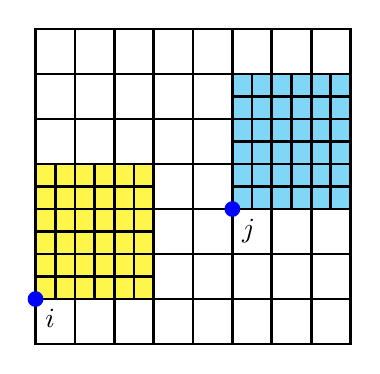
\begin{tikzpicture}[scale=4.0]
    % Define layers
    \pgfdeclarelayer{background}
    \pgfsetlayers{background,main}

    \coordinate (v1_1) at (0.0, 0.0);
    \coordinate (v1_2) at (0.125, 0.0);
    \coordinate (v1_3) at (0.125, 0.14285714285714285);
    \coordinate (v1_4) at (0.0, 0.14285714285714285);
    \draw[black, line width=1.0pt] (v1_1) -- (v1_2) -- (v1_3) -- (v1_4) -- cycle;
    \coordinate (v2_1) at (0.125, 0.0);
    \coordinate (v2_2) at (0.25, 0.0);
    \coordinate (v2_3) at (0.25, 0.14285714285714285);
    \coordinate (v2_4) at (0.125, 0.14285714285714285);
    \draw[black, line width=1.0pt] (v2_1) -- (v2_2) -- (v2_3) -- (v2_4) -- cycle;
    \coordinate (v3_1) at (0.25, 0.0);
    \coordinate (v3_2) at (0.375, 0.0);
    \coordinate (v3_3) at (0.375, 0.14285714285714285);
    \coordinate (v3_4) at (0.25, 0.14285714285714285);
    \draw[black, line width=1.0pt] (v3_1) -- (v3_2) -- (v3_3) -- (v3_4) -- cycle;
    \coordinate (v4_1) at (0.375, 0.0);
    \coordinate (v4_2) at (0.5, 0.0);
    \coordinate (v4_3) at (0.5, 0.14285714285714285);
    \coordinate (v4_4) at (0.375, 0.14285714285714285);
    \draw[black, line width=1.0pt] (v4_1) -- (v4_2) -- (v4_3) -- (v4_4) -- cycle;
    \coordinate (v5_1) at (0.5, 0.0);
    \coordinate (v5_2) at (0.625, 0.0);
    \coordinate (v5_3) at (0.625, 0.14285714285714285);
    \coordinate (v5_4) at (0.5, 0.14285714285714285);
    \draw[black, line width=1.0pt] (v5_1) -- (v5_2) -- (v5_3) -- (v5_4) -- cycle;
    \coordinate (v6_1) at (0.625, 0.0);
    \coordinate (v6_2) at (0.75, 0.0);
    \coordinate (v6_3) at (0.75, 0.14285714285714285);
    \coordinate (v6_4) at (0.625, 0.14285714285714285);
    \draw[black, line width=1.0pt] (v6_1) -- (v6_2) -- (v6_3) -- (v6_4) -- cycle;
    \coordinate (v7_1) at (0.75, 0.0);
    \coordinate (v7_2) at (0.875, 0.0);
    \coordinate (v7_3) at (0.875, 0.14285714285714285);
    \coordinate (v7_4) at (0.75, 0.14285714285714285);
    \draw[black, line width=1.0pt] (v7_1) -- (v7_2) -- (v7_3) -- (v7_4) -- cycle;
    \coordinate (v8_1) at (0.875, 0.0);
    \coordinate (v8_2) at (1.0, 0.0);
    \coordinate (v8_3) at (1.0, 0.14285714285714285);
    \coordinate (v8_4) at (0.875, 0.14285714285714285);
    \draw[black, line width=1.0pt] (v8_1) -- (v8_2) -- (v8_3) -- (v8_4) -- cycle;
    \coordinate (v9_1) at (0.375, 0.14285714285714285);
    \coordinate (v9_2) at (0.5, 0.14285714285714285);
    \coordinate (v9_3) at (0.5, 0.2857142857142857);
    \coordinate (v9_4) at (0.375, 0.2857142857142857);
    \draw[black, line width=1.0pt] (v9_1) -- (v9_2) -- (v9_3) -- (v9_4) -- cycle;
    \coordinate (v10_1) at (0.5, 0.14285714285714285);
    \coordinate (v10_2) at (0.625, 0.14285714285714285);
    \coordinate (v10_3) at (0.625, 0.2857142857142857);
    \coordinate (v10_4) at (0.5, 0.2857142857142857);
    \draw[black, line width=1.0pt] (v10_1) -- (v10_2) -- (v10_3) -- (v10_4) -- cycle;
    \coordinate (v11_1) at (0.625, 0.14285714285714285);
    \coordinate (v11_2) at (0.75, 0.14285714285714285);
    \coordinate (v11_3) at (0.75, 0.2857142857142857);
    \coordinate (v11_4) at (0.625, 0.2857142857142857);
    \draw[black, line width=1.0pt] (v11_1) -- (v11_2) -- (v11_3) -- (v11_4) -- cycle;
    \coordinate (v12_1) at (0.75, 0.14285714285714285);
    \coordinate (v12_2) at (0.875, 0.14285714285714285);
    \coordinate (v12_3) at (0.875, 0.2857142857142857);
    \coordinate (v12_4) at (0.75, 0.2857142857142857);
    \draw[black, line width=1.0pt] (v12_1) -- (v12_2) -- (v12_3) -- (v12_4) -- cycle;
    \coordinate (v13_1) at (0.875, 0.14285714285714285);
    \coordinate (v13_2) at (1.0, 0.14285714285714285);
    \coordinate (v13_3) at (1.0, 0.2857142857142857);
    \coordinate (v13_4) at (0.875, 0.2857142857142857);
    \draw[black, line width=1.0pt] (v13_1) -- (v13_2) -- (v13_3) -- (v13_4) -- cycle;
    \coordinate (v14_1) at (0.375, 0.2857142857142857);
    \coordinate (v14_2) at (0.5, 0.2857142857142857);
    \coordinate (v14_3) at (0.5, 0.42857142857142855);
    \coordinate (v14_4) at (0.375, 0.42857142857142855);
    \draw[black, line width=1.0pt] (v14_1) -- (v14_2) -- (v14_3) -- (v14_4) -- cycle;
    \coordinate (v15_1) at (0.5, 0.2857142857142857);
    \coordinate (v15_2) at (0.625, 0.2857142857142857);
    \coordinate (v15_3) at (0.625, 0.42857142857142855);
    \coordinate (v15_4) at (0.5, 0.42857142857142855);
    \draw[black, line width=1.0pt] (v15_1) -- (v15_2) -- (v15_3) -- (v15_4) -- cycle;
    \coordinate (v16_1) at (0.625, 0.2857142857142857);
    \coordinate (v16_2) at (0.75, 0.2857142857142857);
    \coordinate (v16_3) at (0.75, 0.42857142857142855);
    \coordinate (v16_4) at (0.625, 0.42857142857142855);
    \draw[black, line width=1.0pt] (v16_1) -- (v16_2) -- (v16_3) -- (v16_4) -- cycle;
    \coordinate (v17_1) at (0.75, 0.2857142857142857);
    \coordinate (v17_2) at (0.875, 0.2857142857142857);
    \coordinate (v17_3) at (0.875, 0.42857142857142855);
    \coordinate (v17_4) at (0.75, 0.42857142857142855);
    \draw[black, line width=1.0pt] (v17_1) -- (v17_2) -- (v17_3) -- (v17_4) -- cycle;
    \coordinate (v18_1) at (0.875, 0.2857142857142857);
    \coordinate (v18_2) at (1.0, 0.2857142857142857);
    \coordinate (v18_3) at (1.0, 0.42857142857142855);
    \coordinate (v18_4) at (0.875, 0.42857142857142855);
    \draw[black, line width=1.0pt] (v18_1) -- (v18_2) -- (v18_3) -- (v18_4) -- cycle;
    \coordinate (v19_1) at (0.375, 0.42857142857142855);
    \coordinate (v19_2) at (0.5, 0.42857142857142855);
    \coordinate (v19_3) at (0.5, 0.5714285714285714);
    \coordinate (v19_4) at (0.375, 0.5714285714285714);
    \draw[black, line width=1.0pt] (v19_1) -- (v19_2) -- (v19_3) -- (v19_4) -- cycle;
    \coordinate (v20_1) at (0.5, 0.42857142857142855);
    \coordinate (v20_2) at (0.625, 0.42857142857142855);
    \coordinate (v20_3) at (0.625, 0.5714285714285714);
    \coordinate (v20_4) at (0.5, 0.5714285714285714);
    \draw[black, line width=1.0pt] (v20_1) -- (v20_2) -- (v20_3) -- (v20_4) -- cycle;
    \coordinate (v21_1) at (0.0, 0.5714285714285714);
    \coordinate (v21_2) at (0.125, 0.5714285714285714);
    \coordinate (v21_3) at (0.125, 0.7142857142857143);
    \coordinate (v21_4) at (0.0, 0.7142857142857143);
    \draw[black, line width=1.0pt] (v21_1) -- (v21_2) -- (v21_3) -- (v21_4) -- cycle;
    \coordinate (v22_1) at (0.125, 0.5714285714285714);
    \coordinate (v22_2) at (0.25, 0.5714285714285714);
    \coordinate (v22_3) at (0.25, 0.7142857142857143);
    \coordinate (v22_4) at (0.125, 0.7142857142857143);
    \draw[black, line width=1.0pt] (v22_1) -- (v22_2) -- (v22_3) -- (v22_4) -- cycle;
    \coordinate (v23_1) at (0.25, 0.5714285714285714);
    \coordinate (v23_2) at (0.375, 0.5714285714285714);
    \coordinate (v23_3) at (0.375, 0.7142857142857143);
    \coordinate (v23_4) at (0.25, 0.7142857142857143);
    \draw[black, line width=1.0pt] (v23_1) -- (v23_2) -- (v23_3) -- (v23_4) -- cycle;
    \coordinate (v24_1) at (0.375, 0.5714285714285714);
    \coordinate (v24_2) at (0.5, 0.5714285714285714);
    \coordinate (v24_3) at (0.5, 0.7142857142857143);
    \coordinate (v24_4) at (0.375, 0.7142857142857143);
    \draw[black, line width=1.0pt] (v24_1) -- (v24_2) -- (v24_3) -- (v24_4) -- cycle;
    \coordinate (v25_1) at (0.5, 0.5714285714285714);
    \coordinate (v25_2) at (0.625, 0.5714285714285714);
    \coordinate (v25_3) at (0.625, 0.7142857142857143);
    \coordinate (v25_4) at (0.5, 0.7142857142857143);
    \draw[black, line width=1.0pt] (v25_1) -- (v25_2) -- (v25_3) -- (v25_4) -- cycle;
    \coordinate (v26_1) at (0.0, 0.7142857142857143);
    \coordinate (v26_2) at (0.125, 0.7142857142857143);
    \coordinate (v26_3) at (0.125, 0.8571428571428571);
    \coordinate (v26_4) at (0.0, 0.8571428571428571);
    \draw[black, line width=1.0pt] (v26_1) -- (v26_2) -- (v26_3) -- (v26_4) -- cycle;
    \coordinate (v27_1) at (0.125, 0.7142857142857143);
    \coordinate (v27_2) at (0.25, 0.7142857142857143);
    \coordinate (v27_3) at (0.25, 0.8571428571428571);
    \coordinate (v27_4) at (0.125, 0.8571428571428571);
    \draw[black, line width=1.0pt] (v27_1) -- (v27_2) -- (v27_3) -- (v27_4) -- cycle;
    \coordinate (v28_1) at (0.25, 0.7142857142857143);
    \coordinate (v28_2) at (0.375, 0.7142857142857143);
    \coordinate (v28_3) at (0.375, 0.8571428571428571);
    \coordinate (v28_4) at (0.25, 0.8571428571428571);
    \draw[black, line width=1.0pt] (v28_1) -- (v28_2) -- (v28_3) -- (v28_4) -- cycle;
    \coordinate (v29_1) at (0.375, 0.7142857142857143);
    \coordinate (v29_2) at (0.5, 0.7142857142857143);
    \coordinate (v29_3) at (0.5, 0.8571428571428571);
    \coordinate (v29_4) at (0.375, 0.8571428571428571);
    \draw[black, line width=1.0pt] (v29_1) -- (v29_2) -- (v29_3) -- (v29_4) -- cycle;
    \coordinate (v30_1) at (0.5, 0.7142857142857143);
    \coordinate (v30_2) at (0.625, 0.7142857142857143);
    \coordinate (v30_3) at (0.625, 0.8571428571428571);
    \coordinate (v30_4) at (0.5, 0.8571428571428571);
    \draw[black, line width=1.0pt] (v30_1) -- (v30_2) -- (v30_3) -- (v30_4) -- cycle;
    \coordinate (v31_1) at (0.0, 0.8571428571428571);
    \coordinate (v31_2) at (0.125, 0.8571428571428571);
    \coordinate (v31_3) at (0.125, 1.0);
    \coordinate (v31_4) at (0.0, 1.0);
    \draw[black, line width=1.0pt] (v31_1) -- (v31_2) -- (v31_3) -- (v31_4) -- cycle;
    \coordinate (v32_1) at (0.125, 0.8571428571428571);
    \coordinate (v32_2) at (0.25, 0.8571428571428571);
    \coordinate (v32_3) at (0.25, 1.0);
    \coordinate (v32_4) at (0.125, 1.0);
    \draw[black, line width=1.0pt] (v32_1) -- (v32_2) -- (v32_3) -- (v32_4) -- cycle;
    \coordinate (v33_1) at (0.25, 0.8571428571428571);
    \coordinate (v33_2) at (0.375, 0.8571428571428571);
    \coordinate (v33_3) at (0.375, 1.0);
    \coordinate (v33_4) at (0.25, 1.0);
    \draw[black, line width=1.0pt] (v33_1) -- (v33_2) -- (v33_3) -- (v33_4) -- cycle;
    \coordinate (v34_1) at (0.375, 0.8571428571428571);
    \coordinate (v34_2) at (0.5, 0.8571428571428571);
    \coordinate (v34_3) at (0.5, 1.0);
    \coordinate (v34_4) at (0.375, 1.0);
    \draw[black, line width=1.0pt] (v34_1) -- (v34_2) -- (v34_3) -- (v34_4) -- cycle;
    \coordinate (v35_1) at (0.5, 0.8571428571428571);
    \coordinate (v35_2) at (0.625, 0.8571428571428571);
    \coordinate (v35_3) at (0.625, 1.0);
    \coordinate (v35_4) at (0.5, 1.0);
    \draw[black, line width=1.0pt] (v35_1) -- (v35_2) -- (v35_3) -- (v35_4) -- cycle;
    \coordinate (v36_1) at (0.625, 0.8571428571428571);
    \coordinate (v36_2) at (0.75, 0.8571428571428571);
    \coordinate (v36_3) at (0.75, 1.0);
    \coordinate (v36_4) at (0.625, 1.0);
    \draw[black, line width=1.0pt] (v36_1) -- (v36_2) -- (v36_3) -- (v36_4) -- cycle;
    \coordinate (v37_1) at (0.75, 0.8571428571428571);
    \coordinate (v37_2) at (0.875, 0.8571428571428571);
    \coordinate (v37_3) at (0.875, 1.0);
    \coordinate (v37_4) at (0.75, 1.0);
    \draw[black, line width=1.0pt] (v37_1) -- (v37_2) -- (v37_3) -- (v37_4) -- cycle;
    \coordinate (v38_1) at (0.875, 0.8571428571428571);
    \coordinate (v38_2) at (1.0, 0.8571428571428571);
    \coordinate (v38_3) at (1.0, 1.0);
    \coordinate (v38_4) at (0.875, 1.0);
    \draw[black, line width=1.0pt] (v38_1) -- (v38_2) -- (v38_3) -- (v38_4) -- cycle;
    \coordinate (v39_1) at (0.0, 0.14285714285714285);
    \coordinate (v39_2) at (0.0625, 0.14285714285714285);
    \coordinate (v39_3) at (0.0625, 0.21428571428571427);
    \coordinate (v39_4) at (0.0, 0.21428571428571427);
    \draw[black, line width=1.0pt] (v39_1) -- (v39_2) -- (v39_3) -- (v39_4) -- cycle;
    \coordinate (v40_1) at (0.0625, 0.14285714285714285);
    \coordinate (v40_2) at (0.125, 0.14285714285714285);
    \coordinate (v40_3) at (0.125, 0.21428571428571427);
    \coordinate (v40_4) at (0.0625, 0.21428571428571427);
    \draw[black, line width=1.0pt] (v40_1) -- (v40_2) -- (v40_3) -- (v40_4) -- cycle;
    \coordinate (v41_1) at (0.125, 0.14285714285714285);
    \coordinate (v41_2) at (0.1875, 0.14285714285714285);
    \coordinate (v41_3) at (0.1875, 0.21428571428571427);
    \coordinate (v41_4) at (0.125, 0.21428571428571427);
    \draw[black, line width=1.0pt] (v41_1) -- (v41_2) -- (v41_3) -- (v41_4) -- cycle;
    \coordinate (v42_1) at (0.1875, 0.14285714285714285);
    \coordinate (v42_2) at (0.25, 0.14285714285714285);
    \coordinate (v42_3) at (0.25, 0.21428571428571427);
    \coordinate (v42_4) at (0.1875, 0.21428571428571427);
    \draw[black, line width=1.0pt] (v42_1) -- (v42_2) -- (v42_3) -- (v42_4) -- cycle;
    \coordinate (v43_1) at (0.25, 0.14285714285714285);
    \coordinate (v43_2) at (0.3125, 0.14285714285714285);
    \coordinate (v43_3) at (0.3125, 0.21428571428571427);
    \coordinate (v43_4) at (0.25, 0.21428571428571427);
    \draw[black, line width=1.0pt] (v43_1) -- (v43_2) -- (v43_3) -- (v43_4) -- cycle;
    \coordinate (v44_1) at (0.3125, 0.14285714285714285);
    \coordinate (v44_2) at (0.375, 0.14285714285714285);
    \coordinate (v44_3) at (0.375, 0.21428571428571427);
    \coordinate (v44_4) at (0.3125, 0.21428571428571427);
    \draw[black, line width=1.0pt] (v44_1) -- (v44_2) -- (v44_3) -- (v44_4) -- cycle;
    \coordinate (v45_1) at (0.0, 0.21428571428571427);
    \coordinate (v45_2) at (0.0625, 0.21428571428571427);
    \coordinate (v45_3) at (0.0625, 0.2857142857142857);
    \coordinate (v45_4) at (0.0, 0.2857142857142857);
    \draw[black, line width=1.0pt] (v45_1) -- (v45_2) -- (v45_3) -- (v45_4) -- cycle;
    \coordinate (v46_1) at (0.0625, 0.21428571428571427);
    \coordinate (v46_2) at (0.125, 0.21428571428571427);
    \coordinate (v46_3) at (0.125, 0.2857142857142857);
    \coordinate (v46_4) at (0.0625, 0.2857142857142857);
    \draw[black, line width=1.0pt] (v46_1) -- (v46_2) -- (v46_3) -- (v46_4) -- cycle;
    \coordinate (v47_1) at (0.125, 0.21428571428571427);
    \coordinate (v47_2) at (0.1875, 0.21428571428571427);
    \coordinate (v47_3) at (0.1875, 0.2857142857142857);
    \coordinate (v47_4) at (0.125, 0.2857142857142857);
    \draw[black, line width=1.0pt] (v47_1) -- (v47_2) -- (v47_3) -- (v47_4) -- cycle;
    \coordinate (v48_1) at (0.1875, 0.21428571428571427);
    \coordinate (v48_2) at (0.25, 0.21428571428571427);
    \coordinate (v48_3) at (0.25, 0.2857142857142857);
    \coordinate (v48_4) at (0.1875, 0.2857142857142857);
    \draw[black, line width=1.0pt] (v48_1) -- (v48_2) -- (v48_3) -- (v48_4) -- cycle;
    \coordinate (v49_1) at (0.25, 0.21428571428571427);
    \coordinate (v49_2) at (0.3125, 0.21428571428571427);
    \coordinate (v49_3) at (0.3125, 0.2857142857142857);
    \coordinate (v49_4) at (0.25, 0.2857142857142857);
    \draw[black, line width=1.0pt] (v49_1) -- (v49_2) -- (v49_3) -- (v49_4) -- cycle;
    \coordinate (v50_1) at (0.3125, 0.21428571428571427);
    \coordinate (v50_2) at (0.375, 0.21428571428571427);
    \coordinate (v50_3) at (0.375, 0.2857142857142857);
    \coordinate (v50_4) at (0.3125, 0.2857142857142857);
    \draw[black, line width=1.0pt] (v50_1) -- (v50_2) -- (v50_3) -- (v50_4) -- cycle;
    \coordinate (v51_1) at (0.0, 0.2857142857142857);
    \coordinate (v51_2) at (0.0625, 0.2857142857142857);
    \coordinate (v51_3) at (0.0625, 0.3571428571428571);
    \coordinate (v51_4) at (0.0, 0.3571428571428571);
    \draw[black, line width=1.0pt] (v51_1) -- (v51_2) -- (v51_3) -- (v51_4) -- cycle;
    \coordinate (v52_1) at (0.0625, 0.2857142857142857);
    \coordinate (v52_2) at (0.125, 0.2857142857142857);
    \coordinate (v52_3) at (0.125, 0.3571428571428571);
    \coordinate (v52_4) at (0.0625, 0.3571428571428571);
    \draw[black, line width=1.0pt] (v52_1) -- (v52_2) -- (v52_3) -- (v52_4) -- cycle;
    \coordinate (v53_1) at (0.125, 0.2857142857142857);
    \coordinate (v53_2) at (0.1875, 0.2857142857142857);
    \coordinate (v53_3) at (0.1875, 0.3571428571428571);
    \coordinate (v53_4) at (0.125, 0.3571428571428571);
    \draw[black, line width=1.0pt] (v53_1) -- (v53_2) -- (v53_3) -- (v53_4) -- cycle;
    \coordinate (v54_1) at (0.1875, 0.2857142857142857);
    \coordinate (v54_2) at (0.25, 0.2857142857142857);
    \coordinate (v54_3) at (0.25, 0.3571428571428571);
    \coordinate (v54_4) at (0.1875, 0.3571428571428571);
    \draw[black, line width=1.0pt] (v54_1) -- (v54_2) -- (v54_3) -- (v54_4) -- cycle;
    \coordinate (v55_1) at (0.25, 0.2857142857142857);
    \coordinate (v55_2) at (0.3125, 0.2857142857142857);
    \coordinate (v55_3) at (0.3125, 0.3571428571428571);
    \coordinate (v55_4) at (0.25, 0.3571428571428571);
    \draw[black, line width=1.0pt] (v55_1) -- (v55_2) -- (v55_3) -- (v55_4) -- cycle;
    \coordinate (v56_1) at (0.3125, 0.2857142857142857);
    \coordinate (v56_2) at (0.375, 0.2857142857142857);
    \coordinate (v56_3) at (0.375, 0.3571428571428571);
    \coordinate (v56_4) at (0.3125, 0.3571428571428571);
    \draw[black, line width=1.0pt] (v56_1) -- (v56_2) -- (v56_3) -- (v56_4) -- cycle;
    \coordinate (v57_1) at (0.0, 0.3571428571428571);
    \coordinate (v57_2) at (0.0625, 0.3571428571428571);
    \coordinate (v57_3) at (0.0625, 0.42857142857142855);
    \coordinate (v57_4) at (0.0, 0.42857142857142855);
    \draw[black, line width=1.0pt] (v57_1) -- (v57_2) -- (v57_3) -- (v57_4) -- cycle;
    \coordinate (v58_1) at (0.0625, 0.3571428571428571);
    \coordinate (v58_2) at (0.125, 0.3571428571428571);
    \coordinate (v58_3) at (0.125, 0.42857142857142855);
    \coordinate (v58_4) at (0.0625, 0.42857142857142855);
    \draw[black, line width=1.0pt] (v58_1) -- (v58_2) -- (v58_3) -- (v58_4) -- cycle;
    \coordinate (v59_1) at (0.125, 0.3571428571428571);
    \coordinate (v59_2) at (0.1875, 0.3571428571428571);
    \coordinate (v59_3) at (0.1875, 0.42857142857142855);
    \coordinate (v59_4) at (0.125, 0.42857142857142855);
    \draw[black, line width=1.0pt] (v59_1) -- (v59_2) -- (v59_3) -- (v59_4) -- cycle;
    \coordinate (v60_1) at (0.1875, 0.3571428571428571);
    \coordinate (v60_2) at (0.25, 0.3571428571428571);
    \coordinate (v60_3) at (0.25, 0.42857142857142855);
    \coordinate (v60_4) at (0.1875, 0.42857142857142855);
    \draw[black, line width=1.0pt] (v60_1) -- (v60_2) -- (v60_3) -- (v60_4) -- cycle;
    \coordinate (v61_1) at (0.25, 0.3571428571428571);
    \coordinate (v61_2) at (0.3125, 0.3571428571428571);
    \coordinate (v61_3) at (0.3125, 0.42857142857142855);
    \coordinate (v61_4) at (0.25, 0.42857142857142855);
    \draw[black, line width=1.0pt] (v61_1) -- (v61_2) -- (v61_3) -- (v61_4) -- cycle;
    \coordinate (v62_1) at (0.3125, 0.3571428571428571);
    \coordinate (v62_2) at (0.375, 0.3571428571428571);
    \coordinate (v62_3) at (0.375, 0.42857142857142855);
    \coordinate (v62_4) at (0.3125, 0.42857142857142855);
    \draw[black, line width=1.0pt] (v62_1) -- (v62_2) -- (v62_3) -- (v62_4) -- cycle;
    \coordinate (v63_1) at (0.0, 0.42857142857142855);
    \coordinate (v63_2) at (0.0625, 0.42857142857142855);
    \coordinate (v63_3) at (0.0625, 0.5);
    \coordinate (v63_4) at (0.0, 0.5);
    \draw[black, line width=1.0pt] (v63_1) -- (v63_2) -- (v63_3) -- (v63_4) -- cycle;
    \coordinate (v64_1) at (0.0625, 0.42857142857142855);
    \coordinate (v64_2) at (0.125, 0.42857142857142855);
    \coordinate (v64_3) at (0.125, 0.5);
    \coordinate (v64_4) at (0.0625, 0.5);
    \draw[black, line width=1.0pt] (v64_1) -- (v64_2) -- (v64_3) -- (v64_4) -- cycle;
    \coordinate (v65_1) at (0.125, 0.42857142857142855);
    \coordinate (v65_2) at (0.1875, 0.42857142857142855);
    \coordinate (v65_3) at (0.1875, 0.5);
    \coordinate (v65_4) at (0.125, 0.5);
    \draw[black, line width=1.0pt] (v65_1) -- (v65_2) -- (v65_3) -- (v65_4) -- cycle;
    \coordinate (v66_1) at (0.1875, 0.42857142857142855);
    \coordinate (v66_2) at (0.25, 0.42857142857142855);
    \coordinate (v66_3) at (0.25, 0.5);
    \coordinate (v66_4) at (0.1875, 0.5);
    \draw[black, line width=1.0pt] (v66_1) -- (v66_2) -- (v66_3) -- (v66_4) -- cycle;
    \coordinate (v67_1) at (0.25, 0.42857142857142855);
    \coordinate (v67_2) at (0.3125, 0.42857142857142855);
    \coordinate (v67_3) at (0.3125, 0.5);
    \coordinate (v67_4) at (0.25, 0.5);
    \draw[black, line width=1.0pt] (v67_1) -- (v67_2) -- (v67_3) -- (v67_4) -- cycle;
    \coordinate (v68_1) at (0.3125, 0.42857142857142855);
    \coordinate (v68_2) at (0.375, 0.42857142857142855);
    \coordinate (v68_3) at (0.375, 0.5);
    \coordinate (v68_4) at (0.3125, 0.5);
    \draw[black, line width=1.0pt] (v68_1) -- (v68_2) -- (v68_3) -- (v68_4) -- cycle;
    \coordinate (v69_1) at (0.625, 0.42857142857142855);
    \coordinate (v69_2) at (0.6875, 0.42857142857142855);
    \coordinate (v69_3) at (0.6875, 0.5);
    \coordinate (v69_4) at (0.625, 0.5);
    \draw[black, line width=1.0pt] (v69_1) -- (v69_2) -- (v69_3) -- (v69_4) -- cycle;
    \coordinate (v70_1) at (0.6875, 0.42857142857142855);
    \coordinate (v70_2) at (0.75, 0.42857142857142855);
    \coordinate (v70_3) at (0.75, 0.5);
    \coordinate (v70_4) at (0.6875, 0.5);
    \draw[black, line width=1.0pt] (v70_1) -- (v70_2) -- (v70_3) -- (v70_4) -- cycle;
    \coordinate (v71_1) at (0.75, 0.42857142857142855);
    \coordinate (v71_2) at (0.8125, 0.42857142857142855);
    \coordinate (v71_3) at (0.8125, 0.5);
    \coordinate (v71_4) at (0.75, 0.5);
    \draw[black, line width=1.0pt] (v71_1) -- (v71_2) -- (v71_3) -- (v71_4) -- cycle;
    \coordinate (v72_1) at (0.8125, 0.42857142857142855);
    \coordinate (v72_2) at (0.875, 0.42857142857142855);
    \coordinate (v72_3) at (0.875, 0.5);
    \coordinate (v72_4) at (0.8125, 0.5);
    \draw[black, line width=1.0pt] (v72_1) -- (v72_2) -- (v72_3) -- (v72_4) -- cycle;
    \coordinate (v73_1) at (0.875, 0.42857142857142855);
    \coordinate (v73_2) at (0.9375, 0.42857142857142855);
    \coordinate (v73_3) at (0.9375, 0.5);
    \coordinate (v73_4) at (0.875, 0.5);
    \draw[black, line width=1.0pt] (v73_1) -- (v73_2) -- (v73_3) -- (v73_4) -- cycle;
    \coordinate (v74_1) at (0.9375, 0.42857142857142855);
    \coordinate (v74_2) at (1.0, 0.42857142857142855);
    \coordinate (v74_3) at (1.0, 0.5);
    \coordinate (v74_4) at (0.9375, 0.5);
    \draw[black, line width=1.0pt] (v74_1) -- (v74_2) -- (v74_3) -- (v74_4) -- cycle;
    \coordinate (v75_1) at (0.0, 0.5);
    \coordinate (v75_2) at (0.0625, 0.5);
    \coordinate (v75_3) at (0.0625, 0.5714285714285714);
    \coordinate (v75_4) at (0.0, 0.5714285714285714);
    \draw[black, line width=1.0pt] (v75_1) -- (v75_2) -- (v75_3) -- (v75_4) -- cycle;
    \coordinate (v76_1) at (0.0625, 0.5);
    \coordinate (v76_2) at (0.125, 0.5);
    \coordinate (v76_3) at (0.125, 0.5714285714285714);
    \coordinate (v76_4) at (0.0625, 0.5714285714285714);
    \draw[black, line width=1.0pt] (v76_1) -- (v76_2) -- (v76_3) -- (v76_4) -- cycle;
    \coordinate (v77_1) at (0.125, 0.5);
    \coordinate (v77_2) at (0.1875, 0.5);
    \coordinate (v77_3) at (0.1875, 0.5714285714285714);
    \coordinate (v77_4) at (0.125, 0.5714285714285714);
    \draw[black, line width=1.0pt] (v77_1) -- (v77_2) -- (v77_3) -- (v77_4) -- cycle;
    \coordinate (v78_1) at (0.1875, 0.5);
    \coordinate (v78_2) at (0.25, 0.5);
    \coordinate (v78_3) at (0.25, 0.5714285714285714);
    \coordinate (v78_4) at (0.1875, 0.5714285714285714);
    \draw[black, line width=1.0pt] (v78_1) -- (v78_2) -- (v78_3) -- (v78_4) -- cycle;
    \coordinate (v79_1) at (0.25, 0.5);
    \coordinate (v79_2) at (0.3125, 0.5);
    \coordinate (v79_3) at (0.3125, 0.5714285714285714);
    \coordinate (v79_4) at (0.25, 0.5714285714285714);
    \draw[black, line width=1.0pt] (v79_1) -- (v79_2) -- (v79_3) -- (v79_4) -- cycle;
    \coordinate (v80_1) at (0.3125, 0.5);
    \coordinate (v80_2) at (0.375, 0.5);
    \coordinate (v80_3) at (0.375, 0.5714285714285714);
    \coordinate (v80_4) at (0.3125, 0.5714285714285714);
    \draw[black, line width=1.0pt] (v80_1) -- (v80_2) -- (v80_3) -- (v80_4) -- cycle;
    \coordinate (v81_1) at (0.625, 0.5);
    \coordinate (v81_2) at (0.6875, 0.5);
    \coordinate (v81_3) at (0.6875, 0.5714285714285714);
    \coordinate (v81_4) at (0.625, 0.5714285714285714);
    \draw[black, line width=1.0pt] (v81_1) -- (v81_2) -- (v81_3) -- (v81_4) -- cycle;
    \coordinate (v82_1) at (0.6875, 0.5);
    \coordinate (v82_2) at (0.75, 0.5);
    \coordinate (v82_3) at (0.75, 0.5714285714285714);
    \coordinate (v82_4) at (0.6875, 0.5714285714285714);
    \draw[black, line width=1.0pt] (v82_1) -- (v82_2) -- (v82_3) -- (v82_4) -- cycle;
    \coordinate (v83_1) at (0.75, 0.5);
    \coordinate (v83_2) at (0.8125, 0.5);
    \coordinate (v83_3) at (0.8125, 0.5714285714285714);
    \coordinate (v83_4) at (0.75, 0.5714285714285714);
    \draw[black, line width=1.0pt] (v83_1) -- (v83_2) -- (v83_3) -- (v83_4) -- cycle;
    \coordinate (v84_1) at (0.8125, 0.5);
    \coordinate (v84_2) at (0.875, 0.5);
    \coordinate (v84_3) at (0.875, 0.5714285714285714);
    \coordinate (v84_4) at (0.8125, 0.5714285714285714);
    \draw[black, line width=1.0pt] (v84_1) -- (v84_2) -- (v84_3) -- (v84_4) -- cycle;
    \coordinate (v85_1) at (0.875, 0.5);
    \coordinate (v85_2) at (0.9375, 0.5);
    \coordinate (v85_3) at (0.9375, 0.5714285714285714);
    \coordinate (v85_4) at (0.875, 0.5714285714285714);
    \draw[black, line width=1.0pt] (v85_1) -- (v85_2) -- (v85_3) -- (v85_4) -- cycle;
    \coordinate (v86_1) at (0.9375, 0.5);
    \coordinate (v86_2) at (1.0, 0.5);
    \coordinate (v86_3) at (1.0, 0.5714285714285714);
    \coordinate (v86_4) at (0.9375, 0.5714285714285714);
    \draw[black, line width=1.0pt] (v86_1) -- (v86_2) -- (v86_3) -- (v86_4) -- cycle;
    \coordinate (v87_1) at (0.625, 0.5714285714285714);
    \coordinate (v87_2) at (0.6875, 0.5714285714285714);
    \coordinate (v87_3) at (0.6875, 0.6428571428571428);
    \coordinate (v87_4) at (0.625, 0.6428571428571428);
    \draw[black, line width=1.0pt] (v87_1) -- (v87_2) -- (v87_3) -- (v87_4) -- cycle;
    \coordinate (v88_1) at (0.6875, 0.5714285714285714);
    \coordinate (v88_2) at (0.75, 0.5714285714285714);
    \coordinate (v88_3) at (0.75, 0.6428571428571428);
    \coordinate (v88_4) at (0.6875, 0.6428571428571428);
    \draw[black, line width=1.0pt] (v88_1) -- (v88_2) -- (v88_3) -- (v88_4) -- cycle;
    \coordinate (v89_1) at (0.75, 0.5714285714285714);
    \coordinate (v89_2) at (0.8125, 0.5714285714285714);
    \coordinate (v89_3) at (0.8125, 0.6428571428571428);
    \coordinate (v89_4) at (0.75, 0.6428571428571428);
    \draw[black, line width=1.0pt] (v89_1) -- (v89_2) -- (v89_3) -- (v89_4) -- cycle;
    \coordinate (v90_1) at (0.8125, 0.5714285714285714);
    \coordinate (v90_2) at (0.875, 0.5714285714285714);
    \coordinate (v90_3) at (0.875, 0.6428571428571428);
    \coordinate (v90_4) at (0.8125, 0.6428571428571428);
    \draw[black, line width=1.0pt] (v90_1) -- (v90_2) -- (v90_3) -- (v90_4) -- cycle;
    \coordinate (v91_1) at (0.875, 0.5714285714285714);
    \coordinate (v91_2) at (0.9375, 0.5714285714285714);
    \coordinate (v91_3) at (0.9375, 0.6428571428571428);
    \coordinate (v91_4) at (0.875, 0.6428571428571428);
    \draw[black, line width=1.0pt] (v91_1) -- (v91_2) -- (v91_3) -- (v91_4) -- cycle;
    \coordinate (v92_1) at (0.9375, 0.5714285714285714);
    \coordinate (v92_2) at (1.0, 0.5714285714285714);
    \coordinate (v92_3) at (1.0, 0.6428571428571428);
    \coordinate (v92_4) at (0.9375, 0.6428571428571428);
    \draw[black, line width=1.0pt] (v92_1) -- (v92_2) -- (v92_3) -- (v92_4) -- cycle;
    \coordinate (v93_1) at (0.625, 0.6428571428571428);
    \coordinate (v93_2) at (0.6875, 0.6428571428571428);
    \coordinate (v93_3) at (0.6875, 0.7142857142857143);
    \coordinate (v93_4) at (0.625, 0.7142857142857143);
    \draw[black, line width=1.0pt] (v93_1) -- (v93_2) -- (v93_3) -- (v93_4) -- cycle;
    \coordinate (v94_1) at (0.6875, 0.6428571428571428);
    \coordinate (v94_2) at (0.75, 0.6428571428571428);
    \coordinate (v94_3) at (0.75, 0.7142857142857143);
    \coordinate (v94_4) at (0.6875, 0.7142857142857143);
    \draw[black, line width=1.0pt] (v94_1) -- (v94_2) -- (v94_3) -- (v94_4) -- cycle;
    \coordinate (v95_1) at (0.75, 0.6428571428571428);
    \coordinate (v95_2) at (0.8125, 0.6428571428571428);
    \coordinate (v95_3) at (0.8125, 0.7142857142857143);
    \coordinate (v95_4) at (0.75, 0.7142857142857143);
    \draw[black, line width=1.0pt] (v95_1) -- (v95_2) -- (v95_3) -- (v95_4) -- cycle;
    \coordinate (v96_1) at (0.8125, 0.6428571428571428);
    \coordinate (v96_2) at (0.875, 0.6428571428571428);
    \coordinate (v96_3) at (0.875, 0.7142857142857143);
    \coordinate (v96_4) at (0.8125, 0.7142857142857143);
    \draw[black, line width=1.0pt] (v96_1) -- (v96_2) -- (v96_3) -- (v96_4) -- cycle;
    \coordinate (v97_1) at (0.875, 0.6428571428571428);
    \coordinate (v97_2) at (0.9375, 0.6428571428571428);
    \coordinate (v97_3) at (0.9375, 0.7142857142857143);
    \coordinate (v97_4) at (0.875, 0.7142857142857143);
    \draw[black, line width=1.0pt] (v97_1) -- (v97_2) -- (v97_3) -- (v97_4) -- cycle;
    \coordinate (v98_1) at (0.9375, 0.6428571428571428);
    \coordinate (v98_2) at (1.0, 0.6428571428571428);
    \coordinate (v98_3) at (1.0, 0.7142857142857143);
    \coordinate (v98_4) at (0.9375, 0.7142857142857143);
    \draw[black, line width=1.0pt] (v98_1) -- (v98_2) -- (v98_3) -- (v98_4) -- cycle;
    \coordinate (v99_1) at (0.625, 0.7142857142857143);
    \coordinate (v99_2) at (0.6875, 0.7142857142857143);
    \coordinate (v99_3) at (0.6875, 0.7857142857142857);
    \coordinate (v99_4) at (0.625, 0.7857142857142857);
    \draw[black, line width=1.0pt] (v99_1) -- (v99_2) -- (v99_3) -- (v99_4) -- cycle;
    \coordinate (v100_1) at (0.6875, 0.7142857142857143);
    \coordinate (v100_2) at (0.75, 0.7142857142857143);
    \coordinate (v100_3) at (0.75, 0.7857142857142857);
    \coordinate (v100_4) at (0.6875, 0.7857142857142857);
    \draw[black, line width=1.0pt] (v100_1) -- (v100_2) -- (v100_3) -- (v100_4) -- cycle;
    \coordinate (v101_1) at (0.75, 0.7142857142857143);
    \coordinate (v101_2) at (0.8125, 0.7142857142857143);
    \coordinate (v101_3) at (0.8125, 0.7857142857142857);
    \coordinate (v101_4) at (0.75, 0.7857142857142857);
    \draw[black, line width=1.0pt] (v101_1) -- (v101_2) -- (v101_3) -- (v101_4) -- cycle;
    \coordinate (v102_1) at (0.8125, 0.7142857142857143);
    \coordinate (v102_2) at (0.875, 0.7142857142857143);
    \coordinate (v102_3) at (0.875, 0.7857142857142857);
    \coordinate (v102_4) at (0.8125, 0.7857142857142857);
    \draw[black, line width=1.0pt] (v102_1) -- (v102_2) -- (v102_3) -- (v102_4) -- cycle;
    \coordinate (v103_1) at (0.875, 0.7142857142857143);
    \coordinate (v103_2) at (0.9375, 0.7142857142857143);
    \coordinate (v103_3) at (0.9375, 0.7857142857142857);
    \coordinate (v103_4) at (0.875, 0.7857142857142857);
    \draw[black, line width=1.0pt] (v103_1) -- (v103_2) -- (v103_3) -- (v103_4) -- cycle;
    \coordinate (v104_1) at (0.9375, 0.7142857142857143);
    \coordinate (v104_2) at (1.0, 0.7142857142857143);
    \coordinate (v104_3) at (1.0, 0.7857142857142857);
    \coordinate (v104_4) at (0.9375, 0.7857142857142857);
    \draw[black, line width=1.0pt] (v104_1) -- (v104_2) -- (v104_3) -- (v104_4) -- cycle;
    \coordinate (v105_1) at (0.625, 0.7857142857142857);
    \coordinate (v105_2) at (0.6875, 0.7857142857142857);
    \coordinate (v105_3) at (0.6875, 0.8571428571428571);
    \coordinate (v105_4) at (0.625, 0.8571428571428571);
    \draw[black, line width=1.0pt] (v105_1) -- (v105_2) -- (v105_3) -- (v105_4) -- cycle;
    \coordinate (v106_1) at (0.6875, 0.7857142857142857);
    \coordinate (v106_2) at (0.75, 0.7857142857142857);
    \coordinate (v106_3) at (0.75, 0.8571428571428571);
    \coordinate (v106_4) at (0.6875, 0.8571428571428571);
    \draw[black, line width=1.0pt] (v106_1) -- (v106_2) -- (v106_3) -- (v106_4) -- cycle;
    \coordinate (v107_1) at (0.75, 0.7857142857142857);
    \coordinate (v107_2) at (0.8125, 0.7857142857142857);
    \coordinate (v107_3) at (0.8125, 0.8571428571428571);
    \coordinate (v107_4) at (0.75, 0.8571428571428571);
    \draw[black, line width=1.0pt] (v107_1) -- (v107_2) -- (v107_3) -- (v107_4) -- cycle;
    \coordinate (v108_1) at (0.8125, 0.7857142857142857);
    \coordinate (v108_2) at (0.875, 0.7857142857142857);
    \coordinate (v108_3) at (0.875, 0.8571428571428571);
    \coordinate (v108_4) at (0.8125, 0.8571428571428571);
    \draw[black, line width=1.0pt] (v108_1) -- (v108_2) -- (v108_3) -- (v108_4) -- cycle;
    \coordinate (v109_1) at (0.875, 0.7857142857142857);
    \coordinate (v109_2) at (0.9375, 0.7857142857142857);
    \coordinate (v109_3) at (0.9375, 0.8571428571428571);
    \coordinate (v109_4) at (0.875, 0.8571428571428571);
    \draw[black, line width=1.0pt] (v109_1) -- (v109_2) -- (v109_3) -- (v109_4) -- cycle;
    \coordinate (v110_1) at (0.9375, 0.7857142857142857);
    \coordinate (v110_2) at (1.0, 0.7857142857142857);
    \coordinate (v110_3) at (1.0, 0.8571428571428571);
    \coordinate (v110_4) at (0.9375, 0.8571428571428571);
    \draw[black, line width=1.0pt] (v110_1) -- (v110_2) -- (v110_3) -- (v110_4) -- cycle;

    % Fill the pair support
    \begin{pgfonlayer}{background}
        \fill[yellow, opacity=0.7] (v1_4) rectangle (v19_4);
        \fill[cyan, opacity=0.5] (v20_2) rectangle (v38_2);
    \end{pgfonlayer}

    \node[anchor=north west] at (v1_4) {\(\boldvec{i}\)};
    \node[anchor=north west] at (v20_2) {\(\boldvec{j}\)};
    
    \fill[blue] (v1_4) circle (0.025);
    \fill[blue] (v20_2) circle (0.025);
\end{tikzpicture}

        \caption{}
        \label{fig:problematic-pair-algorithm-case-1-illustration}
    \end{subfigure}
	\hfill
    \begin{subfigure}[t]{0.325\textwidth}
		\centering
		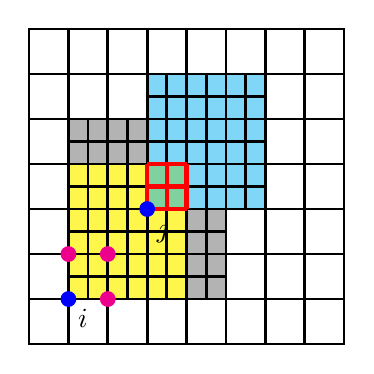
\begin{tikzpicture}[scale=4.0]
    % Define layers
    \pgfdeclarelayer{background}
    \pgfsetlayers{background,main}
    
    \coordinate (v1_1) at (0.0, 0.0);
    \coordinate (v1_2) at (0.125, 0.0);
    \coordinate (v1_3) at (0.125, 0.14285714285714285);
    \coordinate (v1_4) at (0.0, 0.14285714285714285);
    \draw[black, line width=1.0pt] (v1_1) -- (v1_2) -- (v1_3) -- (v1_4) -- cycle;
    \coordinate (v2_1) at (0.125, 0.0);
    \coordinate (v2_2) at (0.25, 0.0);
    \coordinate (v2_3) at (0.25, 0.14285714285714285);
    \coordinate (v2_4) at (0.125, 0.14285714285714285);
    \draw[black, line width=1.0pt] (v2_1) -- (v2_2) -- (v2_3) -- (v2_4) -- cycle;
    \coordinate (v3_1) at (0.25, 0.0);
    \coordinate (v3_2) at (0.375, 0.0);
    \coordinate (v3_3) at (0.375, 0.14285714285714285);
    \coordinate (v3_4) at (0.25, 0.14285714285714285);
    \draw[black, line width=1.0pt] (v3_1) -- (v3_2) -- (v3_3) -- (v3_4) -- cycle;
    \coordinate (v4_1) at (0.375, 0.0);
    \coordinate (v4_2) at (0.5, 0.0);
    \coordinate (v4_3) at (0.5, 0.14285714285714285);
    \coordinate (v4_4) at (0.375, 0.14285714285714285);
    \draw[black, line width=1.0pt] (v4_1) -- (v4_2) -- (v4_3) -- (v4_4) -- cycle;
    \coordinate (v5_1) at (0.5, 0.0);
    \coordinate (v5_2) at (0.625, 0.0);
    \coordinate (v5_3) at (0.625, 0.14285714285714285);
    \coordinate (v5_4) at (0.5, 0.14285714285714285);
    \draw[black, line width=1.0pt] (v5_1) -- (v5_2) -- (v5_3) -- (v5_4) -- cycle;
    \coordinate (v6_1) at (0.625, 0.0);
    \coordinate (v6_2) at (0.75, 0.0);
    \coordinate (v6_3) at (0.75, 0.14285714285714285);
    \coordinate (v6_4) at (0.625, 0.14285714285714285);
    \draw[black, line width=1.0pt] (v6_1) -- (v6_2) -- (v6_3) -- (v6_4) -- cycle;
    \coordinate (v7_1) at (0.75, 0.0);
    \coordinate (v7_2) at (0.875, 0.0);
    \coordinate (v7_3) at (0.875, 0.14285714285714285);
    \coordinate (v7_4) at (0.75, 0.14285714285714285);
    \draw[black, line width=1.0pt] (v7_1) -- (v7_2) -- (v7_3) -- (v7_4) -- cycle;
    \coordinate (v8_1) at (0.875, 0.0);
    \coordinate (v8_2) at (1.0, 0.0);
    \coordinate (v8_3) at (1.0, 0.14285714285714285);
    \coordinate (v8_4) at (0.875, 0.14285714285714285);
    \draw[black, line width=1.0pt] (v8_1) -- (v8_2) -- (v8_3) -- (v8_4) -- cycle;
    \coordinate (v9_1) at (0.0, 0.14285714285714285);
    \coordinate (v9_2) at (0.125, 0.14285714285714285);
    \coordinate (v9_3) at (0.125, 0.2857142857142857);
    \coordinate (v9_4) at (0.0, 0.2857142857142857);
    \draw[black, line width=1.0pt] (v9_1) -- (v9_2) -- (v9_3) -- (v9_4) -- cycle;
    \coordinate (v10_1) at (0.625, 0.14285714285714285);
    \coordinate (v10_2) at (0.75, 0.14285714285714285);
    \coordinate (v10_3) at (0.75, 0.2857142857142857);
    \coordinate (v10_4) at (0.625, 0.2857142857142857);
    \draw[black, line width=1.0pt] (v10_1) -- (v10_2) -- (v10_3) -- (v10_4) -- cycle;
    \coordinate (v11_1) at (0.75, 0.14285714285714285);
    \coordinate (v11_2) at (0.875, 0.14285714285714285);
    \coordinate (v11_3) at (0.875, 0.2857142857142857);
    \coordinate (v11_4) at (0.75, 0.2857142857142857);
    \draw[black, line width=1.0pt] (v11_1) -- (v11_2) -- (v11_3) -- (v11_4) -- cycle;
    \coordinate (v12_1) at (0.875, 0.14285714285714285);
    \coordinate (v12_2) at (1.0, 0.14285714285714285);
    \coordinate (v12_3) at (1.0, 0.2857142857142857);
    \coordinate (v12_4) at (0.875, 0.2857142857142857);
    \draw[black, line width=1.0pt] (v12_1) -- (v12_2) -- (v12_3) -- (v12_4) -- cycle;
    \coordinate (v13_1) at (0.0, 0.2857142857142857);
    \coordinate (v13_2) at (0.125, 0.2857142857142857);
    \coordinate (v13_3) at (0.125, 0.42857142857142855);
    \coordinate (v13_4) at (0.0, 0.42857142857142855);
    \draw[black, line width=1.0pt] (v13_1) -- (v13_2) -- (v13_3) -- (v13_4) -- cycle;
    \coordinate (v14_1) at (0.625, 0.2857142857142857);
    \coordinate (v14_2) at (0.75, 0.2857142857142857);
    \coordinate (v14_3) at (0.75, 0.42857142857142855);
    \coordinate (v14_4) at (0.625, 0.42857142857142855);
    \draw[black, line width=1.0pt] (v14_1) -- (v14_2) -- (v14_3) -- (v14_4) -- cycle;
    \coordinate (v15_1) at (0.75, 0.2857142857142857);
    \coordinate (v15_2) at (0.875, 0.2857142857142857);
    \coordinate (v15_3) at (0.875, 0.42857142857142855);
    \coordinate (v15_4) at (0.75, 0.42857142857142855);
    \draw[black, line width=1.0pt] (v15_1) -- (v15_2) -- (v15_3) -- (v15_4) -- cycle;
    \coordinate (v16_1) at (0.875, 0.2857142857142857);
    \coordinate (v16_2) at (1.0, 0.2857142857142857);
    \coordinate (v16_3) at (1.0, 0.42857142857142855);
    \coordinate (v16_4) at (0.875, 0.42857142857142855);
    \draw[black, line width=1.0pt] (v16_1) -- (v16_2) -- (v16_3) -- (v16_4) -- cycle;
    \coordinate (v17_1) at (0.0, 0.42857142857142855);
    \coordinate (v17_2) at (0.125, 0.42857142857142855);
    \coordinate (v17_3) at (0.125, 0.5714285714285714);
    \coordinate (v17_4) at (0.0, 0.5714285714285714);
    \draw[black, line width=1.0pt] (v17_1) -- (v17_2) -- (v17_3) -- (v17_4) -- cycle;
    \coordinate (v18_1) at (0.75, 0.42857142857142855);
    \coordinate (v18_2) at (0.875, 0.42857142857142855);
    \coordinate (v18_3) at (0.875, 0.5714285714285714);
    \coordinate (v18_4) at (0.75, 0.5714285714285714);
    \draw[black, line width=1.0pt] (v18_1) -- (v18_2) -- (v18_3) -- (v18_4) -- cycle;
    \coordinate (v19_1) at (0.875, 0.42857142857142855);
    \coordinate (v19_2) at (1.0, 0.42857142857142855);
    \coordinate (v19_3) at (1.0, 0.5714285714285714);
    \coordinate (v19_4) at (0.875, 0.5714285714285714);
    \draw[black, line width=1.0pt] (v19_1) -- (v19_2) -- (v19_3) -- (v19_4) -- cycle;
    \coordinate (v20_1) at (0.0, 0.5714285714285714);
    \coordinate (v20_2) at (0.125, 0.5714285714285714);
    \coordinate (v20_3) at (0.125, 0.7142857142857143);
    \coordinate (v20_4) at (0.0, 0.7142857142857143);
    \draw[black, line width=1.0pt] (v20_1) -- (v20_2) -- (v20_3) -- (v20_4) -- cycle;
    \coordinate (v21_1) at (0.75, 0.5714285714285714);
    \coordinate (v21_2) at (0.875, 0.5714285714285714);
    \coordinate (v21_3) at (0.875, 0.7142857142857143);
    \coordinate (v21_4) at (0.75, 0.7142857142857143);
    \draw[black, line width=1.0pt] (v21_1) -- (v21_2) -- (v21_3) -- (v21_4) -- cycle;
    \coordinate (v22_1) at (0.875, 0.5714285714285714);
    \coordinate (v22_2) at (1.0, 0.5714285714285714);
    \coordinate (v22_3) at (1.0, 0.7142857142857143);
    \coordinate (v22_4) at (0.875, 0.7142857142857143);
    \draw[black, line width=1.0pt] (v22_1) -- (v22_2) -- (v22_3) -- (v22_4) -- cycle;
    \coordinate (v23_1) at (0.0, 0.7142857142857143);
    \coordinate (v23_2) at (0.125, 0.7142857142857143);
    \coordinate (v23_3) at (0.125, 0.8571428571428571);
    \coordinate (v23_4) at (0.0, 0.8571428571428571);
    \draw[black, line width=1.0pt] (v23_1) -- (v23_2) -- (v23_3) -- (v23_4) -- cycle;
    \coordinate (v24_1) at (0.125, 0.7142857142857143);
    \coordinate (v24_2) at (0.25, 0.7142857142857143);
    \coordinate (v24_3) at (0.25, 0.8571428571428571);
    \coordinate (v24_4) at (0.125, 0.8571428571428571);
    \draw[black, line width=1.0pt] (v24_1) -- (v24_2) -- (v24_3) -- (v24_4) -- cycle;
    \coordinate (v25_1) at (0.25, 0.7142857142857143);
    \coordinate (v25_2) at (0.375, 0.7142857142857143);
    \coordinate (v25_3) at (0.375, 0.8571428571428571);
    \coordinate (v25_4) at (0.25, 0.8571428571428571);
    \draw[black, line width=1.0pt] (v25_1) -- (v25_2) -- (v25_3) -- (v25_4) -- cycle;
    \coordinate (v26_1) at (0.75, 0.7142857142857143);
    \coordinate (v26_2) at (0.875, 0.7142857142857143);
    \coordinate (v26_3) at (0.875, 0.8571428571428571);
    \coordinate (v26_4) at (0.75, 0.8571428571428571);
    \draw[black, line width=1.0pt] (v26_1) -- (v26_2) -- (v26_3) -- (v26_4) -- cycle;
    \coordinate (v27_1) at (0.875, 0.7142857142857143);
    \coordinate (v27_2) at (1.0, 0.7142857142857143);
    \coordinate (v27_3) at (1.0, 0.8571428571428571);
    \coordinate (v27_4) at (0.875, 0.8571428571428571);
    \draw[black, line width=1.0pt] (v27_1) -- (v27_2) -- (v27_3) -- (v27_4) -- cycle;
    \coordinate (v28_1) at (0.0, 0.8571428571428571);
    \coordinate (v28_2) at (0.125, 0.8571428571428571);
    \coordinate (v28_3) at (0.125, 1.0);
    \coordinate (v28_4) at (0.0, 1.0);
    \draw[black, line width=1.0pt] (v28_1) -- (v28_2) -- (v28_3) -- (v28_4) -- cycle;
    \coordinate (v29_1) at (0.125, 0.8571428571428571);
    \coordinate (v29_2) at (0.25, 0.8571428571428571);
    \coordinate (v29_3) at (0.25, 1.0);
    \coordinate (v29_4) at (0.125, 1.0);
    \draw[black, line width=1.0pt] (v29_1) -- (v29_2) -- (v29_3) -- (v29_4) -- cycle;
    \coordinate (v30_1) at (0.25, 0.8571428571428571);
    \coordinate (v30_2) at (0.375, 0.8571428571428571);
    \coordinate (v30_3) at (0.375, 1.0);
    \coordinate (v30_4) at (0.25, 1.0);
    \draw[black, line width=1.0pt] (v30_1) -- (v30_2) -- (v30_3) -- (v30_4) -- cycle;
    \coordinate (v31_1) at (0.375, 0.8571428571428571);
    \coordinate (v31_2) at (0.5, 0.8571428571428571);
    \coordinate (v31_3) at (0.5, 1.0);
    \coordinate (v31_4) at (0.375, 1.0);
    \draw[black, line width=1.0pt] (v31_1) -- (v31_2) -- (v31_3) -- (v31_4) -- cycle;
    \coordinate (v32_1) at (0.5, 0.8571428571428571);
    \coordinate (v32_2) at (0.625, 0.8571428571428571);
    \coordinate (v32_3) at (0.625, 1.0);
    \coordinate (v32_4) at (0.5, 1.0);
    \draw[black, line width=1.0pt] (v32_1) -- (v32_2) -- (v32_3) -- (v32_4) -- cycle;
    \coordinate (v33_1) at (0.625, 0.8571428571428571);
    \coordinate (v33_2) at (0.75, 0.8571428571428571);
    \coordinate (v33_3) at (0.75, 1.0);
    \coordinate (v33_4) at (0.625, 1.0);
    \draw[black, line width=1.0pt] (v33_1) -- (v33_2) -- (v33_3) -- (v33_4) -- cycle;
    \coordinate (v34_1) at (0.75, 0.8571428571428571);
    \coordinate (v34_2) at (0.875, 0.8571428571428571);
    \coordinate (v34_3) at (0.875, 1.0);
    \coordinate (v34_4) at (0.75, 1.0);
    \draw[black, line width=1.0pt] (v34_1) -- (v34_2) -- (v34_3) -- (v34_4) -- cycle;
    \coordinate (v35_1) at (0.875, 0.8571428571428571);
    \coordinate (v35_2) at (1.0, 0.8571428571428571);
    \coordinate (v35_3) at (1.0, 1.0);
    \coordinate (v35_4) at (0.875, 1.0);
    \draw[black, line width=1.0pt] (v35_1) -- (v35_2) -- (v35_3) -- (v35_4) -- cycle;
    \coordinate (v36_1) at (0.125, 0.14285714285714285);
    \coordinate (v36_2) at (0.1875, 0.14285714285714285);
    \coordinate (v36_3) at (0.1875, 0.21428571428571427);
    \coordinate (v36_4) at (0.125, 0.21428571428571427);
    \draw[black, line width=1.0pt] (v36_1) -- (v36_2) -- (v36_3) -- (v36_4) -- cycle;
    \coordinate (v37_1) at (0.1875, 0.14285714285714285);
    \coordinate (v37_2) at (0.25, 0.14285714285714285);
    \coordinate (v37_3) at (0.25, 0.21428571428571427);
    \coordinate (v37_4) at (0.1875, 0.21428571428571427);
    \draw[black, line width=1.0pt] (v37_1) -- (v37_2) -- (v37_3) -- (v37_4) -- cycle;
    \coordinate (v38_1) at (0.25, 0.14285714285714285);
    \coordinate (v38_2) at (0.3125, 0.14285714285714285);
    \coordinate (v38_3) at (0.3125, 0.21428571428571427);
    \coordinate (v38_4) at (0.25, 0.21428571428571427);
    \draw[black, line width=1.0pt] (v38_1) -- (v38_2) -- (v38_3) -- (v38_4) -- cycle;
    \coordinate (v39_1) at (0.3125, 0.14285714285714285);
    \coordinate (v39_2) at (0.375, 0.14285714285714285);
    \coordinate (v39_3) at (0.375, 0.21428571428571427);
    \coordinate (v39_4) at (0.3125, 0.21428571428571427);
    \draw[black, line width=1.0pt] (v39_1) -- (v39_2) -- (v39_3) -- (v39_4) -- cycle;
    \coordinate (v40_1) at (0.375, 0.14285714285714285);
    \coordinate (v40_2) at (0.4375, 0.14285714285714285);
    \coordinate (v40_3) at (0.4375, 0.21428571428571427);
    \coordinate (v40_4) at (0.375, 0.21428571428571427);
    \draw[black, line width=1.0pt] (v40_1) -- (v40_2) -- (v40_3) -- (v40_4) -- cycle;
    \coordinate (v41_1) at (0.4375, 0.14285714285714285);
    \coordinate (v41_2) at (0.5, 0.14285714285714285);
    \coordinate (v41_3) at (0.5, 0.21428571428571427);
    \coordinate (v41_4) at (0.4375, 0.21428571428571427);
    \draw[black, line width=1.0pt] (v41_1) -- (v41_2) -- (v41_3) -- (v41_4) -- cycle;
    \coordinate (v42_1) at (0.5, 0.14285714285714285);
    \coordinate (v42_2) at (0.5625, 0.14285714285714285);
    \coordinate (v42_3) at (0.5625, 0.21428571428571427);
    \coordinate (v42_4) at (0.5, 0.21428571428571427);
    \draw[black, line width=1.0pt] (v42_1) -- (v42_2) -- (v42_3) -- (v42_4) -- cycle;
    \coordinate (v43_1) at (0.5625, 0.14285714285714285);
    \coordinate (v43_2) at (0.625, 0.14285714285714285);
    \coordinate (v43_3) at (0.625, 0.21428571428571427);
    \coordinate (v43_4) at (0.5625, 0.21428571428571427);
    \draw[black, line width=1.0pt] (v43_1) -- (v43_2) -- (v43_3) -- (v43_4) -- cycle;
    \coordinate (v44_1) at (0.125, 0.21428571428571427);
    \coordinate (v44_2) at (0.1875, 0.21428571428571427);
    \coordinate (v44_3) at (0.1875, 0.2857142857142857);
    \coordinate (v44_4) at (0.125, 0.2857142857142857);
    \draw[black, line width=1.0pt] (v44_1) -- (v44_2) -- (v44_3) -- (v44_4) -- cycle;
    \coordinate (v45_1) at (0.1875, 0.21428571428571427);
    \coordinate (v45_2) at (0.25, 0.21428571428571427);
    \coordinate (v45_3) at (0.25, 0.2857142857142857);
    \coordinate (v45_4) at (0.1875, 0.2857142857142857);
    \draw[black, line width=1.0pt] (v45_1) -- (v45_2) -- (v45_3) -- (v45_4) -- cycle;
    \coordinate (v46_1) at (0.25, 0.21428571428571427);
    \coordinate (v46_2) at (0.3125, 0.21428571428571427);
    \coordinate (v46_3) at (0.3125, 0.2857142857142857);
    \coordinate (v46_4) at (0.25, 0.2857142857142857);
    \draw[black, line width=1.0pt] (v46_1) -- (v46_2) -- (v46_3) -- (v46_4) -- cycle;
    \coordinate (v47_1) at (0.3125, 0.21428571428571427);
    \coordinate (v47_2) at (0.375, 0.21428571428571427);
    \coordinate (v47_3) at (0.375, 0.2857142857142857);
    \coordinate (v47_4) at (0.3125, 0.2857142857142857);
    \draw[black, line width=1.0pt] (v47_1) -- (v47_2) -- (v47_3) -- (v47_4) -- cycle;
    \coordinate (v48_1) at (0.375, 0.21428571428571427);
    \coordinate (v48_2) at (0.4375, 0.21428571428571427);
    \coordinate (v48_3) at (0.4375, 0.2857142857142857);
    \coordinate (v48_4) at (0.375, 0.2857142857142857);
    \draw[black, line width=1.0pt] (v48_1) -- (v48_2) -- (v48_3) -- (v48_4) -- cycle;
    \coordinate (v49_1) at (0.4375, 0.21428571428571427);
    \coordinate (v49_2) at (0.5, 0.21428571428571427);
    \coordinate (v49_3) at (0.5, 0.2857142857142857);
    \coordinate (v49_4) at (0.4375, 0.2857142857142857);
    \draw[black, line width=1.0pt] (v49_1) -- (v49_2) -- (v49_3) -- (v49_4) -- cycle;
    \coordinate (v50_1) at (0.5, 0.21428571428571427);
    \coordinate (v50_2) at (0.5625, 0.21428571428571427);
    \coordinate (v50_3) at (0.5625, 0.2857142857142857);
    \coordinate (v50_4) at (0.5, 0.2857142857142857);
    \draw[black, line width=1.0pt] (v50_1) -- (v50_2) -- (v50_3) -- (v50_4) -- cycle;
    \coordinate (v51_1) at (0.5625, 0.21428571428571427);
    \coordinate (v51_2) at (0.625, 0.21428571428571427);
    \coordinate (v51_3) at (0.625, 0.2857142857142857);
    \coordinate (v51_4) at (0.5625, 0.2857142857142857);
    \draw[black, line width=1.0pt] (v51_1) -- (v51_2) -- (v51_3) -- (v51_4) -- cycle;
    \coordinate (v52_1) at (0.125, 0.2857142857142857);
    \coordinate (v52_2) at (0.1875, 0.2857142857142857);
    \coordinate (v52_3) at (0.1875, 0.3571428571428571);
    \coordinate (v52_4) at (0.125, 0.3571428571428571);
    \draw[black, line width=1.0pt] (v52_1) -- (v52_2) -- (v52_3) -- (v52_4) -- cycle;
    \coordinate (v53_1) at (0.1875, 0.2857142857142857);
    \coordinate (v53_2) at (0.25, 0.2857142857142857);
    \coordinate (v53_3) at (0.25, 0.3571428571428571);
    \coordinate (v53_4) at (0.1875, 0.3571428571428571);
    \draw[black, line width=1.0pt] (v53_1) -- (v53_2) -- (v53_3) -- (v53_4) -- cycle;
    \coordinate (v54_1) at (0.25, 0.2857142857142857);
    \coordinate (v54_2) at (0.3125, 0.2857142857142857);
    \coordinate (v54_3) at (0.3125, 0.3571428571428571);
    \coordinate (v54_4) at (0.25, 0.3571428571428571);
    \draw[black, line width=1.0pt] (v54_1) -- (v54_2) -- (v54_3) -- (v54_4) -- cycle;
    \coordinate (v55_1) at (0.3125, 0.2857142857142857);
    \coordinate (v55_2) at (0.375, 0.2857142857142857);
    \coordinate (v55_3) at (0.375, 0.3571428571428571);
    \coordinate (v55_4) at (0.3125, 0.3571428571428571);
    \draw[black, line width=1.0pt] (v55_1) -- (v55_2) -- (v55_3) -- (v55_4) -- cycle;
    \coordinate (v56_1) at (0.375, 0.2857142857142857);
    \coordinate (v56_2) at (0.4375, 0.2857142857142857);
    \coordinate (v56_3) at (0.4375, 0.3571428571428571);
    \coordinate (v56_4) at (0.375, 0.3571428571428571);
    \draw[black, line width=1.0pt] (v56_1) -- (v56_2) -- (v56_3) -- (v56_4) -- cycle;
    \coordinate (v57_1) at (0.4375, 0.2857142857142857);
    \coordinate (v57_2) at (0.5, 0.2857142857142857);
    \coordinate (v57_3) at (0.5, 0.3571428571428571);
    \coordinate (v57_4) at (0.4375, 0.3571428571428571);
    \draw[black, line width=1.0pt] (v57_1) -- (v57_2) -- (v57_3) -- (v57_4) -- cycle;
    \coordinate (v58_1) at (0.5, 0.2857142857142857);
    \coordinate (v58_2) at (0.5625, 0.2857142857142857);
    \coordinate (v58_3) at (0.5625, 0.3571428571428571);
    \coordinate (v58_4) at (0.5, 0.3571428571428571);
    \draw[black, line width=1.0pt] (v58_1) -- (v58_2) -- (v58_3) -- (v58_4) -- cycle;
    \coordinate (v59_1) at (0.5625, 0.2857142857142857);
    \coordinate (v59_2) at (0.625, 0.2857142857142857);
    \coordinate (v59_3) at (0.625, 0.3571428571428571);
    \coordinate (v59_4) at (0.5625, 0.3571428571428571);
    \draw[black, line width=1.0pt] (v59_1) -- (v59_2) -- (v59_3) -- (v59_4) -- cycle;
    \coordinate (v60_1) at (0.125, 0.3571428571428571);
    \coordinate (v60_2) at (0.1875, 0.3571428571428571);
    \coordinate (v60_3) at (0.1875, 0.42857142857142855);
    \coordinate (v60_4) at (0.125, 0.42857142857142855);
    \draw[black, line width=1.0pt] (v60_1) -- (v60_2) -- (v60_3) -- (v60_4) -- cycle;
    \coordinate (v61_1) at (0.1875, 0.3571428571428571);
    \coordinate (v61_2) at (0.25, 0.3571428571428571);
    \coordinate (v61_3) at (0.25, 0.42857142857142855);
    \coordinate (v61_4) at (0.1875, 0.42857142857142855);
    \draw[black, line width=1.0pt] (v61_1) -- (v61_2) -- (v61_3) -- (v61_4) -- cycle;
    \coordinate (v62_1) at (0.25, 0.3571428571428571);
    \coordinate (v62_2) at (0.3125, 0.3571428571428571);
    \coordinate (v62_3) at (0.3125, 0.42857142857142855);
    \coordinate (v62_4) at (0.25, 0.42857142857142855);
    \draw[black, line width=1.0pt] (v62_1) -- (v62_2) -- (v62_3) -- (v62_4) -- cycle;
    \coordinate (v63_1) at (0.3125, 0.3571428571428571);
    \coordinate (v63_2) at (0.375, 0.3571428571428571);
    \coordinate (v63_3) at (0.375, 0.42857142857142855);
    \coordinate (v63_4) at (0.3125, 0.42857142857142855);
    \draw[black, line width=1.0pt] (v63_1) -- (v63_2) -- (v63_3) -- (v63_4) -- cycle;
    \coordinate (v64_1) at (0.375, 0.3571428571428571);
    \coordinate (v64_2) at (0.4375, 0.3571428571428571);
    \coordinate (v64_3) at (0.4375, 0.42857142857142855);
    \coordinate (v64_4) at (0.375, 0.42857142857142855);
    \draw[black, line width=1.0pt] (v64_1) -- (v64_2) -- (v64_3) -- (v64_4) -- cycle;
    \coordinate (v65_1) at (0.4375, 0.3571428571428571);
    \coordinate (v65_2) at (0.5, 0.3571428571428571);
    \coordinate (v65_3) at (0.5, 0.42857142857142855);
    \coordinate (v65_4) at (0.4375, 0.42857142857142855);
    \draw[black, line width=1.0pt] (v65_1) -- (v65_2) -- (v65_3) -- (v65_4) -- cycle;
    \coordinate (v66_1) at (0.5, 0.3571428571428571);
    \coordinate (v66_2) at (0.5625, 0.3571428571428571);
    \coordinate (v66_3) at (0.5625, 0.42857142857142855);
    \coordinate (v66_4) at (0.5, 0.42857142857142855);
    \draw[black, line width=1.0pt] (v66_1) -- (v66_2) -- (v66_3) -- (v66_4) -- cycle;
    \coordinate (v67_1) at (0.5625, 0.3571428571428571);
    \coordinate (v67_2) at (0.625, 0.3571428571428571);
    \coordinate (v67_3) at (0.625, 0.42857142857142855);
    \coordinate (v67_4) at (0.5625, 0.42857142857142855);
    \draw[black, line width=1.0pt] (v67_1) -- (v67_2) -- (v67_3) -- (v67_4) -- cycle;
    \coordinate (v68_1) at (0.125, 0.42857142857142855);
    \coordinate (v68_2) at (0.1875, 0.42857142857142855);
    \coordinate (v68_3) at (0.1875, 0.5);
    \coordinate (v68_4) at (0.125, 0.5);
    \draw[black, line width=1.0pt] (v68_1) -- (v68_2) -- (v68_3) -- (v68_4) -- cycle;
    \coordinate (v69_1) at (0.1875, 0.42857142857142855);
    \coordinate (v69_2) at (0.25, 0.42857142857142855);
    \coordinate (v69_3) at (0.25, 0.5);
    \coordinate (v69_4) at (0.1875, 0.5);
    \draw[black, line width=1.0pt] (v69_1) -- (v69_2) -- (v69_3) -- (v69_4) -- cycle;
    \coordinate (v70_1) at (0.25, 0.42857142857142855);
    \coordinate (v70_2) at (0.3125, 0.42857142857142855);
    \coordinate (v70_3) at (0.3125, 0.5);
    \coordinate (v70_4) at (0.25, 0.5);
    \draw[black, line width=1.0pt] (v70_1) -- (v70_2) -- (v70_3) -- (v70_4) -- cycle;
    \coordinate (v71_1) at (0.3125, 0.42857142857142855);
    \coordinate (v71_2) at (0.375, 0.42857142857142855);
    \coordinate (v71_3) at (0.375, 0.5);
    \coordinate (v71_4) at (0.3125, 0.5);
    \draw[black, line width=1.0pt] (v71_1) -- (v71_2) -- (v71_3) -- (v71_4) -- cycle;
    \coordinate (v72_1) at (0.375, 0.42857142857142855);
    \coordinate (v72_2) at (0.4375, 0.42857142857142855);
    \coordinate (v72_3) at (0.4375, 0.5);
    \coordinate (v72_4) at (0.375, 0.5);
    \draw[black, line width=1.0pt] (v72_1) -- (v72_2) -- (v72_3) -- (v72_4) -- cycle;
    \coordinate (v73_1) at (0.4375, 0.42857142857142855);
    \coordinate (v73_2) at (0.5, 0.42857142857142855);
    \coordinate (v73_3) at (0.5, 0.5);
    \coordinate (v73_4) at (0.4375, 0.5);
    \draw[black, line width=1.0pt] (v73_1) -- (v73_2) -- (v73_3) -- (v73_4) -- cycle;
    \coordinate (v74_1) at (0.5, 0.42857142857142855);
    \coordinate (v74_2) at (0.5625, 0.42857142857142855);
    \coordinate (v74_3) at (0.5625, 0.5);
    \coordinate (v74_4) at (0.5, 0.5);
    \draw[black, line width=1.0pt] (v74_1) -- (v74_2) -- (v74_3) -- (v74_4) -- cycle;
    \coordinate (v75_1) at (0.5625, 0.42857142857142855);
    \coordinate (v75_2) at (0.625, 0.42857142857142855);
    \coordinate (v75_3) at (0.625, 0.5);
    \coordinate (v75_4) at (0.5625, 0.5);
    \draw[black, line width=1.0pt] (v75_1) -- (v75_2) -- (v75_3) -- (v75_4) -- cycle;
    \coordinate (v76_1) at (0.625, 0.42857142857142855);
    \coordinate (v76_2) at (0.6875, 0.42857142857142855);
    \coordinate (v76_3) at (0.6875, 0.5);
    \coordinate (v76_4) at (0.625, 0.5);
    \draw[black, line width=1.0pt] (v76_1) -- (v76_2) -- (v76_3) -- (v76_4) -- cycle;
    \coordinate (v77_1) at (0.6875, 0.42857142857142855);
    \coordinate (v77_2) at (0.75, 0.42857142857142855);
    \coordinate (v77_3) at (0.75, 0.5);
    \coordinate (v77_4) at (0.6875, 0.5);
    \draw[black, line width=1.0pt] (v77_1) -- (v77_2) -- (v77_3) -- (v77_4) -- cycle;
    \coordinate (v78_1) at (0.125, 0.5);
    \coordinate (v78_2) at (0.1875, 0.5);
    \coordinate (v78_3) at (0.1875, 0.5714285714285714);
    \coordinate (v78_4) at (0.125, 0.5714285714285714);
    \draw[black, line width=1.0pt] (v78_1) -- (v78_2) -- (v78_3) -- (v78_4) -- cycle;
    \coordinate (v79_1) at (0.1875, 0.5);
    \coordinate (v79_2) at (0.25, 0.5);
    \coordinate (v79_3) at (0.25, 0.5714285714285714);
    \coordinate (v79_4) at (0.1875, 0.5714285714285714);
    \draw[black, line width=1.0pt] (v79_1) -- (v79_2) -- (v79_3) -- (v79_4) -- cycle;
    \coordinate (v80_1) at (0.25, 0.5);
    \coordinate (v80_2) at (0.3125, 0.5);
    \coordinate (v80_3) at (0.3125, 0.5714285714285714);
    \coordinate (v80_4) at (0.25, 0.5714285714285714);
    \draw[black, line width=1.0pt] (v80_1) -- (v80_2) -- (v80_3) -- (v80_4) -- cycle;
    \coordinate (v81_1) at (0.3125, 0.5);
    \coordinate (v81_2) at (0.375, 0.5);
    \coordinate (v81_3) at (0.375, 0.5714285714285714);
    \coordinate (v81_4) at (0.3125, 0.5714285714285714);
    \draw[black, line width=1.0pt] (v81_1) -- (v81_2) -- (v81_3) -- (v81_4) -- cycle;
    \coordinate (v82_1) at (0.375, 0.5);
    \coordinate (v82_2) at (0.4375, 0.5);
    \coordinate (v82_3) at (0.4375, 0.5714285714285714);
    \coordinate (v82_4) at (0.375, 0.5714285714285714);
    \draw[black, line width=1.0pt] (v82_1) -- (v82_2) -- (v82_3) -- (v82_4) -- cycle;
    \coordinate (v83_1) at (0.4375, 0.5);
    \coordinate (v83_2) at (0.5, 0.5);
    \coordinate (v83_3) at (0.5, 0.5714285714285714);
    \coordinate (v83_4) at (0.4375, 0.5714285714285714);
    \draw[black, line width=1.0pt] (v83_1) -- (v83_2) -- (v83_3) -- (v83_4) -- cycle;
    \coordinate (v84_1) at (0.5, 0.5);
    \coordinate (v84_2) at (0.5625, 0.5);
    \coordinate (v84_3) at (0.5625, 0.5714285714285714);
    \coordinate (v84_4) at (0.5, 0.5714285714285714);
    \draw[black, line width=1.0pt] (v84_1) -- (v84_2) -- (v84_3) -- (v84_4) -- cycle;
    \coordinate (v85_1) at (0.5625, 0.5);
    \coordinate (v85_2) at (0.625, 0.5);
    \coordinate (v85_3) at (0.625, 0.5714285714285714);
    \coordinate (v85_4) at (0.5625, 0.5714285714285714);
    \draw[black, line width=1.0pt] (v85_1) -- (v85_2) -- (v85_3) -- (v85_4) -- cycle;
    \coordinate (v86_1) at (0.625, 0.5);
    \coordinate (v86_2) at (0.6875, 0.5);
    \coordinate (v86_3) at (0.6875, 0.5714285714285714);
    \coordinate (v86_4) at (0.625, 0.5714285714285714);
    \draw[black, line width=1.0pt] (v86_1) -- (v86_2) -- (v86_3) -- (v86_4) -- cycle;
    \coordinate (v87_1) at (0.6875, 0.5);
    \coordinate (v87_2) at (0.75, 0.5);
    \coordinate (v87_3) at (0.75, 0.5714285714285714);
    \coordinate (v87_4) at (0.6875, 0.5714285714285714);
    \draw[black, line width=1.0pt] (v87_1) -- (v87_2) -- (v87_3) -- (v87_4) -- cycle;
    \coordinate (v88_1) at (0.125, 0.5714285714285714);
    \coordinate (v88_2) at (0.1875, 0.5714285714285714);
    \coordinate (v88_3) at (0.1875, 0.6428571428571428);
    \coordinate (v88_4) at (0.125, 0.6428571428571428);
    \draw[black, line width=1.0pt] (v88_1) -- (v88_2) -- (v88_3) -- (v88_4) -- cycle;
    \coordinate (v89_1) at (0.1875, 0.5714285714285714);
    \coordinate (v89_2) at (0.25, 0.5714285714285714);
    \coordinate (v89_3) at (0.25, 0.6428571428571428);
    \coordinate (v89_4) at (0.1875, 0.6428571428571428);
    \draw[black, line width=1.0pt] (v89_1) -- (v89_2) -- (v89_3) -- (v89_4) -- cycle;
    \coordinate (v90_1) at (0.25, 0.5714285714285714);
    \coordinate (v90_2) at (0.3125, 0.5714285714285714);
    \coordinate (v90_3) at (0.3125, 0.6428571428571428);
    \coordinate (v90_4) at (0.25, 0.6428571428571428);
    \draw[black, line width=1.0pt] (v90_1) -- (v90_2) -- (v90_3) -- (v90_4) -- cycle;
    \coordinate (v91_1) at (0.3125, 0.5714285714285714);
    \coordinate (v91_2) at (0.375, 0.5714285714285714);
    \coordinate (v91_3) at (0.375, 0.6428571428571428);
    \coordinate (v91_4) at (0.3125, 0.6428571428571428);
    \draw[black, line width=1.0pt] (v91_1) -- (v91_2) -- (v91_3) -- (v91_4) -- cycle;
    \coordinate (v92_1) at (0.375, 0.5714285714285714);
    \coordinate (v92_2) at (0.4375, 0.5714285714285714);
    \coordinate (v92_3) at (0.4375, 0.6428571428571428);
    \coordinate (v92_4) at (0.375, 0.6428571428571428);
    \draw[black, line width=1.0pt] (v92_1) -- (v92_2) -- (v92_3) -- (v92_4) -- cycle;
    \coordinate (v93_1) at (0.4375, 0.5714285714285714);
    \coordinate (v93_2) at (0.5, 0.5714285714285714);
    \coordinate (v93_3) at (0.5, 0.6428571428571428);
    \coordinate (v93_4) at (0.4375, 0.6428571428571428);
    \draw[black, line width=1.0pt] (v93_1) -- (v93_2) -- (v93_3) -- (v93_4) -- cycle;
    \coordinate (v94_1) at (0.5, 0.5714285714285714);
    \coordinate (v94_2) at (0.5625, 0.5714285714285714);
    \coordinate (v94_3) at (0.5625, 0.6428571428571428);
    \coordinate (v94_4) at (0.5, 0.6428571428571428);
    \draw[black, line width=1.0pt] (v94_1) -- (v94_2) -- (v94_3) -- (v94_4) -- cycle;
    \coordinate (v95_1) at (0.5625, 0.5714285714285714);
    \coordinate (v95_2) at (0.625, 0.5714285714285714);
    \coordinate (v95_3) at (0.625, 0.6428571428571428);
    \coordinate (v95_4) at (0.5625, 0.6428571428571428);
    \draw[black, line width=1.0pt] (v95_1) -- (v95_2) -- (v95_3) -- (v95_4) -- cycle;
    \coordinate (v96_1) at (0.625, 0.5714285714285714);
    \coordinate (v96_2) at (0.6875, 0.5714285714285714);
    \coordinate (v96_3) at (0.6875, 0.6428571428571428);
    \coordinate (v96_4) at (0.625, 0.6428571428571428);
    \draw[black, line width=1.0pt] (v96_1) -- (v96_2) -- (v96_3) -- (v96_4) -- cycle;
    \coordinate (v97_1) at (0.6875, 0.5714285714285714);
    \coordinate (v97_2) at (0.75, 0.5714285714285714);
    \coordinate (v97_3) at (0.75, 0.6428571428571428);
    \coordinate (v97_4) at (0.6875, 0.6428571428571428);
    \draw[black, line width=1.0pt] (v97_1) -- (v97_2) -- (v97_3) -- (v97_4) -- cycle;
    \coordinate (v98_1) at (0.125, 0.6428571428571428);
    \coordinate (v98_2) at (0.1875, 0.6428571428571428);
    \coordinate (v98_3) at (0.1875, 0.7142857142857143);
    \coordinate (v98_4) at (0.125, 0.7142857142857143);
    \draw[black, line width=1.0pt] (v98_1) -- (v98_2) -- (v98_3) -- (v98_4) -- cycle;
    \coordinate (v99_1) at (0.1875, 0.6428571428571428);
    \coordinate (v99_2) at (0.25, 0.6428571428571428);
    \coordinate (v99_3) at (0.25, 0.7142857142857143);
    \coordinate (v99_4) at (0.1875, 0.7142857142857143);
    \draw[black, line width=1.0pt] (v99_1) -- (v99_2) -- (v99_3) -- (v99_4) -- cycle;
    \coordinate (v100_1) at (0.25, 0.6428571428571428);
    \coordinate (v100_2) at (0.3125, 0.6428571428571428);
    \coordinate (v100_3) at (0.3125, 0.7142857142857143);
    \coordinate (v100_4) at (0.25, 0.7142857142857143);
    \draw[black, line width=1.0pt] (v100_1) -- (v100_2) -- (v100_3) -- (v100_4) -- cycle;
    \coordinate (v101_1) at (0.3125, 0.6428571428571428);
    \coordinate (v101_2) at (0.375, 0.6428571428571428);
    \coordinate (v101_3) at (0.375, 0.7142857142857143);
    \coordinate (v101_4) at (0.3125, 0.7142857142857143);
    \draw[black, line width=1.0pt] (v101_1) -- (v101_2) -- (v101_3) -- (v101_4) -- cycle;
    \coordinate (v102_1) at (0.375, 0.6428571428571428);
    \coordinate (v102_2) at (0.4375, 0.6428571428571428);
    \coordinate (v102_3) at (0.4375, 0.7142857142857143);
    \coordinate (v102_4) at (0.375, 0.7142857142857143);
    \draw[black, line width=1.0pt] (v102_1) -- (v102_2) -- (v102_3) -- (v102_4) -- cycle;
    \coordinate (v103_1) at (0.4375, 0.6428571428571428);
    \coordinate (v103_2) at (0.5, 0.6428571428571428);
    \coordinate (v103_3) at (0.5, 0.7142857142857143);
    \coordinate (v103_4) at (0.4375, 0.7142857142857143);
    \draw[black, line width=1.0pt] (v103_1) -- (v103_2) -- (v103_3) -- (v103_4) -- cycle;
    \coordinate (v104_1) at (0.5, 0.6428571428571428);
    \coordinate (v104_2) at (0.5625, 0.6428571428571428);
    \coordinate (v104_3) at (0.5625, 0.7142857142857143);
    \coordinate (v104_4) at (0.5, 0.7142857142857143);
    \draw[black, line width=1.0pt] (v104_1) -- (v104_2) -- (v104_3) -- (v104_4) -- cycle;
    \coordinate (v105_1) at (0.5625, 0.6428571428571428);
    \coordinate (v105_2) at (0.625, 0.6428571428571428);
    \coordinate (v105_3) at (0.625, 0.7142857142857143);
    \coordinate (v105_4) at (0.5625, 0.7142857142857143);
    \draw[black, line width=1.0pt] (v105_1) -- (v105_2) -- (v105_3) -- (v105_4) -- cycle;
    \coordinate (v106_1) at (0.625, 0.6428571428571428);
    \coordinate (v106_2) at (0.6875, 0.6428571428571428);
    \coordinate (v106_3) at (0.6875, 0.7142857142857143);
    \coordinate (v106_4) at (0.625, 0.7142857142857143);
    \draw[black, line width=1.0pt] (v106_1) -- (v106_2) -- (v106_3) -- (v106_4) -- cycle;
    \coordinate (v107_1) at (0.6875, 0.6428571428571428);
    \coordinate (v107_2) at (0.75, 0.6428571428571428);
    \coordinate (v107_3) at (0.75, 0.7142857142857143);
    \coordinate (v107_4) at (0.6875, 0.7142857142857143);
    \draw[black, line width=1.0pt] (v107_1) -- (v107_2) -- (v107_3) -- (v107_4) -- cycle;
    \coordinate (v108_1) at (0.375, 0.7142857142857143);
    \coordinate (v108_2) at (0.4375, 0.7142857142857143);
    \coordinate (v108_3) at (0.4375, 0.7857142857142857);
    \coordinate (v108_4) at (0.375, 0.7857142857142857);
    \draw[black, line width=1.0pt] (v108_1) -- (v108_2) -- (v108_3) -- (v108_4) -- cycle;
    \coordinate (v109_1) at (0.4375, 0.7142857142857143);
    \coordinate (v109_2) at (0.5, 0.7142857142857143);
    \coordinate (v109_3) at (0.5, 0.7857142857142857);
    \coordinate (v109_4) at (0.4375, 0.7857142857142857);
    \draw[black, line width=1.0pt] (v109_1) -- (v109_2) -- (v109_3) -- (v109_4) -- cycle;
    \coordinate (v110_1) at (0.5, 0.7142857142857143);
    \coordinate (v110_2) at (0.5625, 0.7142857142857143);
    \coordinate (v110_3) at (0.5625, 0.7857142857142857);
    \coordinate (v110_4) at (0.5, 0.7857142857142857);
    \draw[black, line width=1.0pt] (v110_1) -- (v110_2) -- (v110_3) -- (v110_4) -- cycle;
    \coordinate (v111_1) at (0.5625, 0.7142857142857143);
    \coordinate (v111_2) at (0.625, 0.7142857142857143);
    \coordinate (v111_3) at (0.625, 0.7857142857142857);
    \coordinate (v111_4) at (0.5625, 0.7857142857142857);
    \draw[black, line width=1.0pt] (v111_1) -- (v111_2) -- (v111_3) -- (v111_4) -- cycle;
    \coordinate (v112_1) at (0.625, 0.7142857142857143);
    \coordinate (v112_2) at (0.6875, 0.7142857142857143);
    \coordinate (v112_3) at (0.6875, 0.7857142857142857);
    \coordinate (v112_4) at (0.625, 0.7857142857142857);
    \draw[black, line width=1.0pt] (v112_1) -- (v112_2) -- (v112_3) -- (v112_4) -- cycle;
    \coordinate (v113_1) at (0.6875, 0.7142857142857143);
    \coordinate (v113_2) at (0.75, 0.7142857142857143);
    \coordinate (v113_3) at (0.75, 0.7857142857142857);
    \coordinate (v113_4) at (0.6875, 0.7857142857142857);
    \draw[black, line width=1.0pt] (v113_1) -- (v113_2) -- (v113_3) -- (v113_4) -- cycle;
    \coordinate (v114_1) at (0.375, 0.7857142857142857);
    \coordinate (v114_2) at (0.4375, 0.7857142857142857);
    \coordinate (v114_3) at (0.4375, 0.8571428571428571);
    \coordinate (v114_4) at (0.375, 0.8571428571428571);
    \draw[black, line width=1.0pt] (v114_1) -- (v114_2) -- (v114_3) -- (v114_4) -- cycle;
    \coordinate (v115_1) at (0.4375, 0.7857142857142857);
    \coordinate (v115_2) at (0.5, 0.7857142857142857);
    \coordinate (v115_3) at (0.5, 0.8571428571428571);
    \coordinate (v115_4) at (0.4375, 0.8571428571428571);
    \draw[black, line width=1.0pt] (v115_1) -- (v115_2) -- (v115_3) -- (v115_4) -- cycle;
    \coordinate (v116_1) at (0.5, 0.7857142857142857);
    \coordinate (v116_2) at (0.5625, 0.7857142857142857);
    \coordinate (v116_3) at (0.5625, 0.8571428571428571);
    \coordinate (v116_4) at (0.5, 0.8571428571428571);
    \draw[black, line width=1.0pt] (v116_1) -- (v116_2) -- (v116_3) -- (v116_4) -- cycle;
    \coordinate (v117_1) at (0.5625, 0.7857142857142857);
    \coordinate (v117_2) at (0.625, 0.7857142857142857);
    \coordinate (v117_3) at (0.625, 0.8571428571428571);
    \coordinate (v117_4) at (0.5625, 0.8571428571428571);
    \draw[black, line width=1.0pt] (v117_1) -- (v117_2) -- (v117_3) -- (v117_4) -- cycle;
    \coordinate (v118_1) at (0.625, 0.7857142857142857);
    \coordinate (v118_2) at (0.6875, 0.7857142857142857);
    \coordinate (v118_3) at (0.6875, 0.8571428571428571);
    \coordinate (v118_4) at (0.625, 0.8571428571428571);
    \draw[black, line width=1.0pt] (v118_1) -- (v118_2) -- (v118_3) -- (v118_4) -- cycle;
    \coordinate (v119_1) at (0.6875, 0.7857142857142857);
    \coordinate (v119_2) at (0.75, 0.7857142857142857);
    \coordinate (v119_3) at (0.75, 0.8571428571428571);
    \coordinate (v119_4) at (0.6875, 0.8571428571428571);
    \draw[black, line width=1.0pt] (v119_1) -- (v119_2) -- (v119_3) -- (v119_4) -- cycle;

    % Fill the pair support
    \begin{pgfonlayer}{background}
        \fill[gray, opacity=0.6] (v88_1) rectangle (v102_4);
        \fill[gray, opacity=0.6] (v5_4) rectangle (v14_4);
        \fill[yellow, opacity=0.7] (v9_2) rectangle (v84_4);
        \fill[cyan, opacity=0.5] (v72_1) rectangle (v33_2);
    \end{pgfonlayer}

    \draw[red, line width=1.5] (v72_1) -- (v74_1);
    \draw[red, line width=1.5] (v72_4) -- (v74_4);
    \draw[red, line width=1.5] (v72_1) -- (v82_4);
    \draw[red, line width=1.5] (v72_2) -- (v82_3);
    \draw[red, line width=1.5] (v82_4) -- (v84_4);
    \draw[red, line width=1.5] (v74_1) -- (v84_4);  

    \node[anchor=north west] at (v9_2) {\(\boldvec{i}\)};
    
    \node[anchor=north west] at (v72_1) {\(\boldvec{j}\)};
    
    \fill[magenta] (v3_4) circle (0.025);
    \fill[magenta] (v9_3) circle (0.025);
    \fill[magenta] (v54_1) circle (0.025);
    %\draw[magenta, line width=1.0pt] (v9_2) -- (v3_4) --  (v54_1) -- (v9_3) -- cycle;
    \fill[blue] (v9_2) circle (0.025);
    \fill[blue] (v72_1) circle (0.025);

\end{tikzpicture}

		\caption{}
		\label{fig:problematic-pair-algorithm-case-2-illustration}
    \end{subfigure}
	\hfill
    \begin{subfigure}[t]{0.325\textwidth}
        \centering
        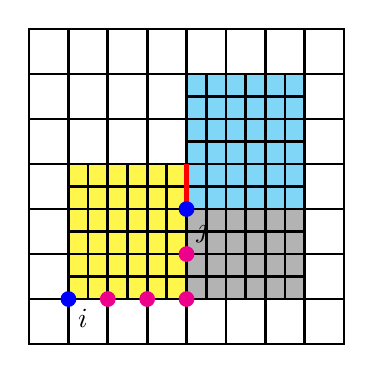
\begin{tikzpicture}[scale=4.0]
    % Define layers
    \pgfdeclarelayer{background}
    \pgfsetlayers{background,main}

    \coordinate (v1_1) at (0.0, 0.0);
    \coordinate (v1_2) at (0.125, 0.0);
    \coordinate (v1_3) at (0.125, 0.14285714285714285);
    \coordinate (v1_4) at (0.0, 0.14285714285714285);
    \draw[black, line width=1.0pt] (v1_1) -- (v1_2) -- (v1_3) -- (v1_4) -- cycle;
    \coordinate (v2_1) at (0.125, 0.0);
    \coordinate (v2_2) at (0.25, 0.0);
    \coordinate (v2_3) at (0.25, 0.14285714285714285);
    \coordinate (v2_4) at (0.125, 0.14285714285714285);
    \draw[black, line width=1.0pt] (v2_1) -- (v2_2) -- (v2_3) -- (v2_4) -- cycle;
    \coordinate (v3_1) at (0.25, 0.0);
    \coordinate (v3_2) at (0.375, 0.0);
    \coordinate (v3_3) at (0.375, 0.14285714285714285);
    \coordinate (v3_4) at (0.25, 0.14285714285714285);
    \draw[black, line width=1.0pt] (v3_1) -- (v3_2) -- (v3_3) -- (v3_4) -- cycle;
    \coordinate (v4_1) at (0.375, 0.0);
    \coordinate (v4_2) at (0.5, 0.0);
    \coordinate (v4_3) at (0.5, 0.14285714285714285);
    \coordinate (v4_4) at (0.375, 0.14285714285714285);
    \draw[black, line width=1.0pt] (v4_1) -- (v4_2) -- (v4_3) -- (v4_4) -- cycle;
    \coordinate (v5_1) at (0.5, 0.0);
    \coordinate (v5_2) at (0.625, 0.0);
    \coordinate (v5_3) at (0.625, 0.14285714285714285);
    \coordinate (v5_4) at (0.5, 0.14285714285714285);
    \draw[black, line width=1.0pt] (v5_1) -- (v5_2) -- (v5_3) -- (v5_4) -- cycle;
    \coordinate (v6_1) at (0.625, 0.0);
    \coordinate (v6_2) at (0.75, 0.0);
    \coordinate (v6_3) at (0.75, 0.14285714285714285);
    \coordinate (v6_4) at (0.625, 0.14285714285714285);
    \draw[black, line width=1.0pt] (v6_1) -- (v6_2) -- (v6_3) -- (v6_4) -- cycle;
    \coordinate (v7_1) at (0.75, 0.0);
    \coordinate (v7_2) at (0.875, 0.0);
    \coordinate (v7_3) at (0.875, 0.14285714285714285);
    \coordinate (v7_4) at (0.75, 0.14285714285714285);
    \draw[black, line width=1.0pt] (v7_1) -- (v7_2) -- (v7_3) -- (v7_4) -- cycle;
    \coordinate (v8_1) at (0.875, 0.0);
    \coordinate (v8_2) at (1.0, 0.0);
    \coordinate (v8_3) at (1.0, 0.14285714285714285);
    \coordinate (v8_4) at (0.875, 0.14285714285714285);
    \draw[black, line width=1.0pt] (v8_1) -- (v8_2) -- (v8_3) -- (v8_4) -- cycle;
    \coordinate (v9_1) at (0.0, 0.14285714285714285);
    \coordinate (v9_2) at (0.125, 0.14285714285714285);
    \coordinate (v9_3) at (0.125, 0.2857142857142857);
    \coordinate (v9_4) at (0.0, 0.2857142857142857);
    \draw[black, line width=1.0pt] (v9_1) -- (v9_2) -- (v9_3) -- (v9_4) -- cycle;
    \coordinate (v10_1) at (0.875, 0.14285714285714285);
    \coordinate (v10_2) at (1.0, 0.14285714285714285);
    \coordinate (v10_3) at (1.0, 0.2857142857142857);
    \coordinate (v10_4) at (0.875, 0.2857142857142857);
    \draw[black, line width=1.0pt] (v10_1) -- (v10_2) -- (v10_3) -- (v10_4) -- cycle;
    \coordinate (v11_1) at (0.0, 0.2857142857142857);
    \coordinate (v11_2) at (0.125, 0.2857142857142857);
    \coordinate (v11_3) at (0.125, 0.42857142857142855);
    \coordinate (v11_4) at (0.0, 0.42857142857142855);
    \draw[black, line width=1.0pt] (v11_1) -- (v11_2) -- (v11_3) -- (v11_4) -- cycle;
    \coordinate (v12_1) at (0.875, 0.2857142857142857);
    \coordinate (v12_2) at (1.0, 0.2857142857142857);
    \coordinate (v12_3) at (1.0, 0.42857142857142855);
    \coordinate (v12_4) at (0.875, 0.42857142857142855);
    \draw[black, line width=1.0pt] (v12_1) -- (v12_2) -- (v12_3) -- (v12_4) -- cycle;
    \coordinate (v13_1) at (0.0, 0.42857142857142855);
    \coordinate (v13_2) at (0.125, 0.42857142857142855);
    \coordinate (v13_3) at (0.125, 0.5714285714285714);
    \coordinate (v13_4) at (0.0, 0.5714285714285714);
    \draw[black, line width=1.0pt] (v13_1) -- (v13_2) -- (v13_3) -- (v13_4) -- cycle;
    \coordinate (v14_1) at (0.875, 0.42857142857142855);
    \coordinate (v14_2) at (1.0, 0.42857142857142855);
    \coordinate (v14_3) at (1.0, 0.5714285714285714);
    \coordinate (v14_4) at (0.875, 0.5714285714285714);
    \draw[black, line width=1.0pt] (v14_1) -- (v14_2) -- (v14_3) -- (v14_4) -- cycle;
    \coordinate (v15_1) at (0.0, 0.5714285714285714);
    \coordinate (v15_2) at (0.125, 0.5714285714285714);
    \coordinate (v15_3) at (0.125, 0.7142857142857143);
    \coordinate (v15_4) at (0.0, 0.7142857142857143);
    \draw[black, line width=1.0pt] (v15_1) -- (v15_2) -- (v15_3) -- (v15_4) -- cycle;
    \coordinate (v16_1) at (0.125, 0.5714285714285714);
    \coordinate (v16_2) at (0.25, 0.5714285714285714);
    \coordinate (v16_3) at (0.25, 0.7142857142857143);
    \coordinate (v16_4) at (0.125, 0.7142857142857143);
    \draw[black, line width=1.0pt] (v16_1) -- (v16_2) -- (v16_3) -- (v16_4) -- cycle;
    \coordinate (v17_1) at (0.25, 0.5714285714285714);
    \coordinate (v17_2) at (0.375, 0.5714285714285714);
    \coordinate (v17_3) at (0.375, 0.7142857142857143);
    \coordinate (v17_4) at (0.25, 0.7142857142857143);
    \draw[black, line width=1.0pt] (v17_1) -- (v17_2) -- (v17_3) -- (v17_4) -- cycle;
    \coordinate (v18_1) at (0.375, 0.5714285714285714);
    \coordinate (v18_2) at (0.5, 0.5714285714285714);
    \coordinate (v18_3) at (0.5, 0.7142857142857143);
    \coordinate (v18_4) at (0.375, 0.7142857142857143);
    \draw[black, line width=1.0pt] (v18_1) -- (v18_2) -- (v18_3) -- (v18_4) -- cycle;
    \coordinate (v19_1) at (0.875, 0.5714285714285714);
    \coordinate (v19_2) at (1.0, 0.5714285714285714);
    \coordinate (v19_3) at (1.0, 0.7142857142857143);
    \coordinate (v19_4) at (0.875, 0.7142857142857143);
    \draw[black, line width=1.0pt] (v19_1) -- (v19_2) -- (v19_3) -- (v19_4) -- cycle;
    \coordinate (v20_1) at (0.0, 0.7142857142857143);
    \coordinate (v20_2) at (0.125, 0.7142857142857143);
    \coordinate (v20_3) at (0.125, 0.8571428571428571);
    \coordinate (v20_4) at (0.0, 0.8571428571428571);
    \draw[black, line width=1.0pt] (v20_1) -- (v20_2) -- (v20_3) -- (v20_4) -- cycle;
    \coordinate (v21_1) at (0.125, 0.7142857142857143);
    \coordinate (v21_2) at (0.25, 0.7142857142857143);
    \coordinate (v21_3) at (0.25, 0.8571428571428571);
    \coordinate (v21_4) at (0.125, 0.8571428571428571);
    \draw[black, line width=1.0pt] (v21_1) -- (v21_2) -- (v21_3) -- (v21_4) -- cycle;
    \coordinate (v22_1) at (0.25, 0.7142857142857143);
    \coordinate (v22_2) at (0.375, 0.7142857142857143);
    \coordinate (v22_3) at (0.375, 0.8571428571428571);
    \coordinate (v22_4) at (0.25, 0.8571428571428571);
    \draw[black, line width=1.0pt] (v22_1) -- (v22_2) -- (v22_3) -- (v22_4) -- cycle;
    \coordinate (v23_1) at (0.375, 0.7142857142857143);
    \coordinate (v23_2) at (0.5, 0.7142857142857143);
    \coordinate (v23_3) at (0.5, 0.8571428571428571);
    \coordinate (v23_4) at (0.375, 0.8571428571428571);
    \draw[black, line width=1.0pt] (v23_1) -- (v23_2) -- (v23_3) -- (v23_4) -- cycle;
    \coordinate (v24_1) at (0.875, 0.7142857142857143);
    \coordinate (v24_2) at (1.0, 0.7142857142857143);
    \coordinate (v24_3) at (1.0, 0.8571428571428571);
    \coordinate (v24_4) at (0.875, 0.8571428571428571);
    \draw[black, line width=1.0pt] (v24_1) -- (v24_2) -- (v24_3) -- (v24_4) -- cycle;
    \coordinate (v25_1) at (0.0, 0.8571428571428571);
    \coordinate (v25_2) at (0.125, 0.8571428571428571);
    \coordinate (v25_3) at (0.125, 1.0);
    \coordinate (v25_4) at (0.0, 1.0);
    \draw[black, line width=1.0pt] (v25_1) -- (v25_2) -- (v25_3) -- (v25_4) -- cycle;
    \coordinate (v26_1) at (0.125, 0.8571428571428571);
    \coordinate (v26_2) at (0.25, 0.8571428571428571);
    \coordinate (v26_3) at (0.25, 1.0);
    \coordinate (v26_4) at (0.125, 1.0);
    \draw[black, line width=1.0pt] (v26_1) -- (v26_2) -- (v26_3) -- (v26_4) -- cycle;
    \coordinate (v27_1) at (0.25, 0.8571428571428571);
    \coordinate (v27_2) at (0.375, 0.8571428571428571);
    \coordinate (v27_3) at (0.375, 1.0);
    \coordinate (v27_4) at (0.25, 1.0);
    \draw[black, line width=1.0pt] (v27_1) -- (v27_2) -- (v27_3) -- (v27_4) -- cycle;
    \coordinate (v28_1) at (0.375, 0.8571428571428571);
    \coordinate (v28_2) at (0.5, 0.8571428571428571);
    \coordinate (v28_3) at (0.5, 1.0);
    \coordinate (v28_4) at (0.375, 1.0);
    \draw[black, line width=1.0pt] (v28_1) -- (v28_2) -- (v28_3) -- (v28_4) -- cycle;
    \coordinate (v29_1) at (0.5, 0.8571428571428571);
    \coordinate (v29_2) at (0.625, 0.8571428571428571);
    \coordinate (v29_3) at (0.625, 1.0);
    \coordinate (v29_4) at (0.5, 1.0);
    \draw[black, line width=1.0pt] (v29_1) -- (v29_2) -- (v29_3) -- (v29_4) -- cycle;
    \coordinate (v30_1) at (0.625, 0.8571428571428571);
    \coordinate (v30_2) at (0.75, 0.8571428571428571);
    \coordinate (v30_3) at (0.75, 1.0);
    \coordinate (v30_4) at (0.625, 1.0);
    \draw[black, line width=1.0pt] (v30_1) -- (v30_2) -- (v30_3) -- (v30_4) -- cycle;
    \coordinate (v31_1) at (0.75, 0.8571428571428571);
    \coordinate (v31_2) at (0.875, 0.8571428571428571);
    \coordinate (v31_3) at (0.875, 1.0);
    \coordinate (v31_4) at (0.75, 1.0);
    \draw[black, line width=1.0pt] (v31_1) -- (v31_2) -- (v31_3) -- (v31_4) -- cycle;
    \coordinate (v32_1) at (0.875, 0.8571428571428571);
    \coordinate (v32_2) at (1.0, 0.8571428571428571);
    \coordinate (v32_3) at (1.0, 1.0);
    \coordinate (v32_4) at (0.875, 1.0);
    \draw[black, line width=1.0pt] (v32_1) -- (v32_2) -- (v32_3) -- (v32_4) -- cycle;
    \coordinate (v33_1) at (0.125, 0.14285714285714285);
    \coordinate (v33_2) at (0.1875, 0.14285714285714285);
    \coordinate (v33_3) at (0.1875, 0.21428571428571427);
    \coordinate (v33_4) at (0.125, 0.21428571428571427);
    \draw[black, line width=1.0pt] (v33_1) -- (v33_2) -- (v33_3) -- (v33_4) -- cycle;
    \coordinate (v34_1) at (0.1875, 0.14285714285714285);
    \coordinate (v34_2) at (0.25, 0.14285714285714285);
    \coordinate (v34_3) at (0.25, 0.21428571428571427);
    \coordinate (v34_4) at (0.1875, 0.21428571428571427);
    \draw[black, line width=1.0pt] (v34_1) -- (v34_2) -- (v34_3) -- (v34_4) -- cycle;
    \coordinate (v35_1) at (0.25, 0.14285714285714285);
    \coordinate (v35_2) at (0.3125, 0.14285714285714285);
    \coordinate (v35_3) at (0.3125, 0.21428571428571427);
    \coordinate (v35_4) at (0.25, 0.21428571428571427);
    \draw[black, line width=1.0pt] (v35_1) -- (v35_2) -- (v35_3) -- (v35_4) -- cycle;
    \coordinate (v36_1) at (0.3125, 0.14285714285714285);
    \coordinate (v36_2) at (0.375, 0.14285714285714285);
    \coordinate (v36_3) at (0.375, 0.21428571428571427);
    \coordinate (v36_4) at (0.3125, 0.21428571428571427);
    \draw[black, line width=1.0pt] (v36_1) -- (v36_2) -- (v36_3) -- (v36_4) -- cycle;
    \coordinate (v37_1) at (0.375, 0.14285714285714285);
    \coordinate (v37_2) at (0.4375, 0.14285714285714285);
    \coordinate (v37_3) at (0.4375, 0.21428571428571427);
    \coordinate (v37_4) at (0.375, 0.21428571428571427);
    \draw[black, line width=1.0pt] (v37_1) -- (v37_2) -- (v37_3) -- (v37_4) -- cycle;
    \coordinate (v38_1) at (0.4375, 0.14285714285714285);
    \coordinate (v38_2) at (0.5, 0.14285714285714285);
    \coordinate (v38_3) at (0.5, 0.21428571428571427);
    \coordinate (v38_4) at (0.4375, 0.21428571428571427);
    \draw[black, line width=1.0pt] (v38_1) -- (v38_2) -- (v38_3) -- (v38_4) -- cycle;
    \coordinate (v39_1) at (0.5, 0.14285714285714285);
    \coordinate (v39_2) at (0.5625, 0.14285714285714285);
    \coordinate (v39_3) at (0.5625, 0.21428571428571427);
    \coordinate (v39_4) at (0.5, 0.21428571428571427);
    \draw[black, line width=1.0pt] (v39_1) -- (v39_2) -- (v39_3) -- (v39_4) -- cycle;
    \coordinate (v40_1) at (0.5625, 0.14285714285714285);
    \coordinate (v40_2) at (0.625, 0.14285714285714285);
    \coordinate (v40_3) at (0.625, 0.21428571428571427);
    \coordinate (v40_4) at (0.5625, 0.21428571428571427);
    \draw[black, line width=1.0pt] (v40_1) -- (v40_2) -- (v40_3) -- (v40_4) -- cycle;
    \coordinate (v41_1) at (0.625, 0.14285714285714285);
    \coordinate (v41_2) at (0.6875, 0.14285714285714285);
    \coordinate (v41_3) at (0.6875, 0.21428571428571427);
    \coordinate (v41_4) at (0.625, 0.21428571428571427);
    \draw[black, line width=1.0pt] (v41_1) -- (v41_2) -- (v41_3) -- (v41_4) -- cycle;
    \coordinate (v42_1) at (0.6875, 0.14285714285714285);
    \coordinate (v42_2) at (0.75, 0.14285714285714285);
    \coordinate (v42_3) at (0.75, 0.21428571428571427);
    \coordinate (v42_4) at (0.6875, 0.21428571428571427);
    \draw[black, line width=1.0pt] (v42_1) -- (v42_2) -- (v42_3) -- (v42_4) -- cycle;
    \coordinate (v43_1) at (0.75, 0.14285714285714285);
    \coordinate (v43_2) at (0.8125, 0.14285714285714285);
    \coordinate (v43_3) at (0.8125, 0.21428571428571427);
    \coordinate (v43_4) at (0.75, 0.21428571428571427);
    \draw[black, line width=1.0pt] (v43_1) -- (v43_2) -- (v43_3) -- (v43_4) -- cycle;
    \coordinate (v44_1) at (0.8125, 0.14285714285714285);
    \coordinate (v44_2) at (0.875, 0.14285714285714285);
    \coordinate (v44_3) at (0.875, 0.21428571428571427);
    \coordinate (v44_4) at (0.8125, 0.21428571428571427);
    \draw[black, line width=1.0pt] (v44_1) -- (v44_2) -- (v44_3) -- (v44_4) -- cycle;
    \coordinate (v45_1) at (0.125, 0.21428571428571427);
    \coordinate (v45_2) at (0.1875, 0.21428571428571427);
    \coordinate (v45_3) at (0.1875, 0.2857142857142857);
    \coordinate (v45_4) at (0.125, 0.2857142857142857);
    \draw[black, line width=1.0pt] (v45_1) -- (v45_2) -- (v45_3) -- (v45_4) -- cycle;
    \coordinate (v46_1) at (0.1875, 0.21428571428571427);
    \coordinate (v46_2) at (0.25, 0.21428571428571427);
    \coordinate (v46_3) at (0.25, 0.2857142857142857);
    \coordinate (v46_4) at (0.1875, 0.2857142857142857);
    \draw[black, line width=1.0pt] (v46_1) -- (v46_2) -- (v46_3) -- (v46_4) -- cycle;
    \coordinate (v47_1) at (0.25, 0.21428571428571427);
    \coordinate (v47_2) at (0.3125, 0.21428571428571427);
    \coordinate (v47_3) at (0.3125, 0.2857142857142857);
    \coordinate (v47_4) at (0.25, 0.2857142857142857);
    \draw[black, line width=1.0pt] (v47_1) -- (v47_2) -- (v47_3) -- (v47_4) -- cycle;
    \coordinate (v48_1) at (0.3125, 0.21428571428571427);
    \coordinate (v48_2) at (0.375, 0.21428571428571427);
    \coordinate (v48_3) at (0.375, 0.2857142857142857);
    \coordinate (v48_4) at (0.3125, 0.2857142857142857);
    \draw[black, line width=1.0pt] (v48_1) -- (v48_2) -- (v48_3) -- (v48_4) -- cycle;
    \coordinate (v49_1) at (0.375, 0.21428571428571427);
    \coordinate (v49_2) at (0.4375, 0.21428571428571427);
    \coordinate (v49_3) at (0.4375, 0.2857142857142857);
    \coordinate (v49_4) at (0.375, 0.2857142857142857);
    \draw[black, line width=1.0pt] (v49_1) -- (v49_2) -- (v49_3) -- (v49_4) -- cycle;
    \coordinate (v50_1) at (0.4375, 0.21428571428571427);
    \coordinate (v50_2) at (0.5, 0.21428571428571427);
    \coordinate (v50_3) at (0.5, 0.2857142857142857);
    \coordinate (v50_4) at (0.4375, 0.2857142857142857);
    \draw[black, line width=1.0pt] (v50_1) -- (v50_2) -- (v50_3) -- (v50_4) -- cycle;
    \coordinate (v51_1) at (0.5, 0.21428571428571427);
    \coordinate (v51_2) at (0.5625, 0.21428571428571427);
    \coordinate (v51_3) at (0.5625, 0.2857142857142857);
    \coordinate (v51_4) at (0.5, 0.2857142857142857);
    \draw[black, line width=1.0pt] (v51_1) -- (v51_2) -- (v51_3) -- (v51_4) -- cycle;
    \coordinate (v52_1) at (0.5625, 0.21428571428571427);
    \coordinate (v52_2) at (0.625, 0.21428571428571427);
    \coordinate (v52_3) at (0.625, 0.2857142857142857);
    \coordinate (v52_4) at (0.5625, 0.2857142857142857);
    \draw[black, line width=1.0pt] (v52_1) -- (v52_2) -- (v52_3) -- (v52_4) -- cycle;
    \coordinate (v53_1) at (0.625, 0.21428571428571427);
    \coordinate (v53_2) at (0.6875, 0.21428571428571427);
    \coordinate (v53_3) at (0.6875, 0.2857142857142857);
    \coordinate (v53_4) at (0.625, 0.2857142857142857);
    \draw[black, line width=1.0pt] (v53_1) -- (v53_2) -- (v53_3) -- (v53_4) -- cycle;
    \coordinate (v54_1) at (0.6875, 0.21428571428571427);
    \coordinate (v54_2) at (0.75, 0.21428571428571427);
    \coordinate (v54_3) at (0.75, 0.2857142857142857);
    \coordinate (v54_4) at (0.6875, 0.2857142857142857);
    \draw[black, line width=1.0pt] (v54_1) -- (v54_2) -- (v54_3) -- (v54_4) -- cycle;
    \coordinate (v55_1) at (0.75, 0.21428571428571427);
    \coordinate (v55_2) at (0.8125, 0.21428571428571427);
    \coordinate (v55_3) at (0.8125, 0.2857142857142857);
    \coordinate (v55_4) at (0.75, 0.2857142857142857);
    \draw[black, line width=1.0pt] (v55_1) -- (v55_2) -- (v55_3) -- (v55_4) -- cycle;
    \coordinate (v56_1) at (0.8125, 0.21428571428571427);
    \coordinate (v56_2) at (0.875, 0.21428571428571427);
    \coordinate (v56_3) at (0.875, 0.2857142857142857);
    \coordinate (v56_4) at (0.8125, 0.2857142857142857);
    \draw[black, line width=1.0pt] (v56_1) -- (v56_2) -- (v56_3) -- (v56_4) -- cycle;
    \coordinate (v57_1) at (0.125, 0.2857142857142857);
    \coordinate (v57_2) at (0.1875, 0.2857142857142857);
    \coordinate (v57_3) at (0.1875, 0.3571428571428571);
    \coordinate (v57_4) at (0.125, 0.3571428571428571);
    \draw[black, line width=1.0pt] (v57_1) -- (v57_2) -- (v57_3) -- (v57_4) -- cycle;
    \coordinate (v58_1) at (0.1875, 0.2857142857142857);
    \coordinate (v58_2) at (0.25, 0.2857142857142857);
    \coordinate (v58_3) at (0.25, 0.3571428571428571);
    \coordinate (v58_4) at (0.1875, 0.3571428571428571);
    \draw[black, line width=1.0pt] (v58_1) -- (v58_2) -- (v58_3) -- (v58_4) -- cycle;
    \coordinate (v59_1) at (0.25, 0.2857142857142857);
    \coordinate (v59_2) at (0.3125, 0.2857142857142857);
    \coordinate (v59_3) at (0.3125, 0.3571428571428571);
    \coordinate (v59_4) at (0.25, 0.3571428571428571);
    \draw[black, line width=1.0pt] (v59_1) -- (v59_2) -- (v59_3) -- (v59_4) -- cycle;
    \coordinate (v60_1) at (0.3125, 0.2857142857142857);
    \coordinate (v60_2) at (0.375, 0.2857142857142857);
    \coordinate (v60_3) at (0.375, 0.3571428571428571);
    \coordinate (v60_4) at (0.3125, 0.3571428571428571);
    \draw[black, line width=1.0pt] (v60_1) -- (v60_2) -- (v60_3) -- (v60_4) -- cycle;
    \coordinate (v61_1) at (0.375, 0.2857142857142857);
    \coordinate (v61_2) at (0.4375, 0.2857142857142857);
    \coordinate (v61_3) at (0.4375, 0.3571428571428571);
    \coordinate (v61_4) at (0.375, 0.3571428571428571);
    \draw[black, line width=1.0pt] (v61_1) -- (v61_2) -- (v61_3) -- (v61_4) -- cycle;
    \coordinate (v62_1) at (0.4375, 0.2857142857142857);
    \coordinate (v62_2) at (0.5, 0.2857142857142857);
    \coordinate (v62_3) at (0.5, 0.3571428571428571);
    \coordinate (v62_4) at (0.4375, 0.3571428571428571);
    \draw[black, line width=1.0pt] (v62_1) -- (v62_2) -- (v62_3) -- (v62_4) -- cycle;
    \coordinate (v63_1) at (0.5, 0.2857142857142857);
    \coordinate (v63_2) at (0.5625, 0.2857142857142857);
    \coordinate (v63_3) at (0.5625, 0.3571428571428571);
    \coordinate (v63_4) at (0.5, 0.3571428571428571);
    \draw[black, line width=1.0pt] (v63_1) -- (v63_2) -- (v63_3) -- (v63_4) -- cycle;
    \coordinate (v64_1) at (0.5625, 0.2857142857142857);
    \coordinate (v64_2) at (0.625, 0.2857142857142857);
    \coordinate (v64_3) at (0.625, 0.3571428571428571);
    \coordinate (v64_4) at (0.5625, 0.3571428571428571);
    \draw[black, line width=1.0pt] (v64_1) -- (v64_2) -- (v64_3) -- (v64_4) -- cycle;
    \coordinate (v65_1) at (0.625, 0.2857142857142857);
    \coordinate (v65_2) at (0.6875, 0.2857142857142857);
    \coordinate (v65_3) at (0.6875, 0.3571428571428571);
    \coordinate (v65_4) at (0.625, 0.3571428571428571);
    \draw[black, line width=1.0pt] (v65_1) -- (v65_2) -- (v65_3) -- (v65_4) -- cycle;
    \coordinate (v66_1) at (0.6875, 0.2857142857142857);
    \coordinate (v66_2) at (0.75, 0.2857142857142857);
    \coordinate (v66_3) at (0.75, 0.3571428571428571);
    \coordinate (v66_4) at (0.6875, 0.3571428571428571);
    \draw[black, line width=1.0pt] (v66_1) -- (v66_2) -- (v66_3) -- (v66_4) -- cycle;
    \coordinate (v67_1) at (0.75, 0.2857142857142857);
    \coordinate (v67_2) at (0.8125, 0.2857142857142857);
    \coordinate (v67_3) at (0.8125, 0.3571428571428571);
    \coordinate (v67_4) at (0.75, 0.3571428571428571);
    \draw[black, line width=1.0pt] (v67_1) -- (v67_2) -- (v67_3) -- (v67_4) -- cycle;
    \coordinate (v68_1) at (0.8125, 0.2857142857142857);
    \coordinate (v68_2) at (0.875, 0.2857142857142857);
    \coordinate (v68_3) at (0.875, 0.3571428571428571);
    \coordinate (v68_4) at (0.8125, 0.3571428571428571);
    \draw[black, line width=1.0pt] (v68_1) -- (v68_2) -- (v68_3) -- (v68_4) -- cycle;
    \coordinate (v69_1) at (0.125, 0.3571428571428571);
    \coordinate (v69_2) at (0.1875, 0.3571428571428571);
    \coordinate (v69_3) at (0.1875, 0.42857142857142855);
    \coordinate (v69_4) at (0.125, 0.42857142857142855);
    \draw[black, line width=1.0pt] (v69_1) -- (v69_2) -- (v69_3) -- (v69_4) -- cycle;
    \coordinate (v70_1) at (0.1875, 0.3571428571428571);
    \coordinate (v70_2) at (0.25, 0.3571428571428571);
    \coordinate (v70_3) at (0.25, 0.42857142857142855);
    \coordinate (v70_4) at (0.1875, 0.42857142857142855);
    \draw[black, line width=1.0pt] (v70_1) -- (v70_2) -- (v70_3) -- (v70_4) -- cycle;
    \coordinate (v71_1) at (0.25, 0.3571428571428571);
    \coordinate (v71_2) at (0.3125, 0.3571428571428571);
    \coordinate (v71_3) at (0.3125, 0.42857142857142855);
    \coordinate (v71_4) at (0.25, 0.42857142857142855);
    \draw[black, line width=1.0pt] (v71_1) -- (v71_2) -- (v71_3) -- (v71_4) -- cycle;
    \coordinate (v72_1) at (0.3125, 0.3571428571428571);
    \coordinate (v72_2) at (0.375, 0.3571428571428571);
    \coordinate (v72_3) at (0.375, 0.42857142857142855);
    \coordinate (v72_4) at (0.3125, 0.42857142857142855);
    \draw[black, line width=1.0pt] (v72_1) -- (v72_2) -- (v72_3) -- (v72_4) -- cycle;
    \coordinate (v73_1) at (0.375, 0.3571428571428571);
    \coordinate (v73_2) at (0.4375, 0.3571428571428571);
    \coordinate (v73_3) at (0.4375, 0.42857142857142855);
    \coordinate (v73_4) at (0.375, 0.42857142857142855);
    \draw[black, line width=1.0pt] (v73_1) -- (v73_2) -- (v73_3) -- (v73_4) -- cycle;
    \coordinate (v74_1) at (0.4375, 0.3571428571428571);
    \coordinate (v74_2) at (0.5, 0.3571428571428571);
    \coordinate (v74_3) at (0.5, 0.42857142857142855);
    \coordinate (v74_4) at (0.4375, 0.42857142857142855);
    \draw[black, line width=1.0pt] (v74_1) -- (v74_2) -- (v74_3) -- (v74_4) -- cycle;
    \coordinate (v75_1) at (0.5, 0.3571428571428571);
    \coordinate (v75_2) at (0.5625, 0.3571428571428571);
    \coordinate (v75_3) at (0.5625, 0.42857142857142855);
    \coordinate (v75_4) at (0.5, 0.42857142857142855);
    \draw[black, line width=1.0pt] (v75_1) -- (v75_2) -- (v75_3) -- (v75_4) -- cycle;
    \coordinate (v76_1) at (0.5625, 0.3571428571428571);
    \coordinate (v76_2) at (0.625, 0.3571428571428571);
    \coordinate (v76_3) at (0.625, 0.42857142857142855);
    \coordinate (v76_4) at (0.5625, 0.42857142857142855);
    \draw[black, line width=1.0pt] (v76_1) -- (v76_2) -- (v76_3) -- (v76_4) -- cycle;
    \coordinate (v77_1) at (0.625, 0.3571428571428571);
    \coordinate (v77_2) at (0.6875, 0.3571428571428571);
    \coordinate (v77_3) at (0.6875, 0.42857142857142855);
    \coordinate (v77_4) at (0.625, 0.42857142857142855);
    \draw[black, line width=1.0pt] (v77_1) -- (v77_2) -- (v77_3) -- (v77_4) -- cycle;
    \coordinate (v78_1) at (0.6875, 0.3571428571428571);
    \coordinate (v78_2) at (0.75, 0.3571428571428571);
    \coordinate (v78_3) at (0.75, 0.42857142857142855);
    \coordinate (v78_4) at (0.6875, 0.42857142857142855);
    \draw[black, line width=1.0pt] (v78_1) -- (v78_2) -- (v78_3) -- (v78_4) -- cycle;
    \coordinate (v79_1) at (0.75, 0.3571428571428571);
    \coordinate (v79_2) at (0.8125, 0.3571428571428571);
    \coordinate (v79_3) at (0.8125, 0.42857142857142855);
    \coordinate (v79_4) at (0.75, 0.42857142857142855);
    \draw[black, line width=1.0pt] (v79_1) -- (v79_2) -- (v79_3) -- (v79_4) -- cycle;
    \coordinate (v80_1) at (0.8125, 0.3571428571428571);
    \coordinate (v80_2) at (0.875, 0.3571428571428571);
    \coordinate (v80_3) at (0.875, 0.42857142857142855);
    \coordinate (v80_4) at (0.8125, 0.42857142857142855);
    \draw[black, line width=1.0pt] (v80_1) -- (v80_2) -- (v80_3) -- (v80_4) -- cycle;
    \coordinate (v81_1) at (0.125, 0.42857142857142855);
    \coordinate (v81_2) at (0.1875, 0.42857142857142855);
    \coordinate (v81_3) at (0.1875, 0.5);
    \coordinate (v81_4) at (0.125, 0.5);
    \draw[black, line width=1.0pt] (v81_1) -- (v81_2) -- (v81_3) -- (v81_4) -- cycle;
    \coordinate (v82_1) at (0.1875, 0.42857142857142855);
    \coordinate (v82_2) at (0.25, 0.42857142857142855);
    \coordinate (v82_3) at (0.25, 0.5);
    \coordinate (v82_4) at (0.1875, 0.5);
    \draw[black, line width=1.0pt] (v82_1) -- (v82_2) -- (v82_3) -- (v82_4) -- cycle;
    \coordinate (v83_1) at (0.25, 0.42857142857142855);
    \coordinate (v83_2) at (0.3125, 0.42857142857142855);
    \coordinate (v83_3) at (0.3125, 0.5);
    \coordinate (v83_4) at (0.25, 0.5);
    \draw[black, line width=1.0pt] (v83_1) -- (v83_2) -- (v83_3) -- (v83_4) -- cycle;
    \coordinate (v84_1) at (0.3125, 0.42857142857142855);
    \coordinate (v84_2) at (0.375, 0.42857142857142855);
    \coordinate (v84_3) at (0.375, 0.5);
    \coordinate (v84_4) at (0.3125, 0.5);
    \draw[black, line width=1.0pt] (v84_1) -- (v84_2) -- (v84_3) -- (v84_4) -- cycle;
    \coordinate (v85_1) at (0.375, 0.42857142857142855);
    \coordinate (v85_2) at (0.4375, 0.42857142857142855);
    \coordinate (v85_3) at (0.4375, 0.5);
    \coordinate (v85_4) at (0.375, 0.5);
    \draw[black, line width=1.0pt] (v85_1) -- (v85_2) -- (v85_3) -- (v85_4) -- cycle;
    \coordinate (v86_1) at (0.4375, 0.42857142857142855);
    \coordinate (v86_2) at (0.5, 0.42857142857142855);
    \coordinate (v86_3) at (0.5, 0.5);
    \coordinate (v86_4) at (0.4375, 0.5);
    \draw[black, line width=1.0pt] (v86_1) -- (v86_2) -- (v86_3) -- (v86_4) -- cycle;
    \coordinate (v87_1) at (0.5, 0.42857142857142855);
    \coordinate (v87_2) at (0.5625, 0.42857142857142855);
    \coordinate (v87_3) at (0.5625, 0.5);
    \coordinate (v87_4) at (0.5, 0.5);
    \draw[black, line width=1.0pt] (v87_1) -- (v87_2) -- (v87_3) -- (v87_4) -- cycle;
    \coordinate (v88_1) at (0.5625, 0.42857142857142855);
    \coordinate (v88_2) at (0.625, 0.42857142857142855);
    \coordinate (v88_3) at (0.625, 0.5);
    \coordinate (v88_4) at (0.5625, 0.5);
    \draw[black, line width=1.0pt] (v88_1) -- (v88_2) -- (v88_3) -- (v88_4) -- cycle;
    \coordinate (v89_1) at (0.625, 0.42857142857142855);
    \coordinate (v89_2) at (0.6875, 0.42857142857142855);
    \coordinate (v89_3) at (0.6875, 0.5);
    \coordinate (v89_4) at (0.625, 0.5);
    \draw[black, line width=1.0pt] (v89_1) -- (v89_2) -- (v89_3) -- (v89_4) -- cycle;
    \coordinate (v90_1) at (0.6875, 0.42857142857142855);
    \coordinate (v90_2) at (0.75, 0.42857142857142855);
    \coordinate (v90_3) at (0.75, 0.5);
    \coordinate (v90_4) at (0.6875, 0.5);
    \draw[black, line width=1.0pt] (v90_1) -- (v90_2) -- (v90_3) -- (v90_4) -- cycle;
    \coordinate (v91_1) at (0.75, 0.42857142857142855);
    \coordinate (v91_2) at (0.8125, 0.42857142857142855);
    \coordinate (v91_3) at (0.8125, 0.5);
    \coordinate (v91_4) at (0.75, 0.5);
    \draw[black, line width=1.0pt] (v91_1) -- (v91_2) -- (v91_3) -- (v91_4) -- cycle;
    \coordinate (v92_1) at (0.8125, 0.42857142857142855);
    \coordinate (v92_2) at (0.875, 0.42857142857142855);
    \coordinate (v92_3) at (0.875, 0.5);
    \coordinate (v92_4) at (0.8125, 0.5);
    \draw[black, line width=1.0pt] (v92_1) -- (v92_2) -- (v92_3) -- (v92_4) -- cycle;
    \coordinate (v93_1) at (0.125, 0.5);
    \coordinate (v93_2) at (0.1875, 0.5);
    \coordinate (v93_3) at (0.1875, 0.5714285714285714);
    \coordinate (v93_4) at (0.125, 0.5714285714285714);
    \draw[black, line width=1.0pt] (v93_1) -- (v93_2) -- (v93_3) -- (v93_4) -- cycle;
    \coordinate (v94_1) at (0.1875, 0.5);
    \coordinate (v94_2) at (0.25, 0.5);
    \coordinate (v94_3) at (0.25, 0.5714285714285714);
    \coordinate (v94_4) at (0.1875, 0.5714285714285714);
    \draw[black, line width=1.0pt] (v94_1) -- (v94_2) -- (v94_3) -- (v94_4) -- cycle;
    \coordinate (v95_1) at (0.25, 0.5);
    \coordinate (v95_2) at (0.3125, 0.5);
    \coordinate (v95_3) at (0.3125, 0.5714285714285714);
    \coordinate (v95_4) at (0.25, 0.5714285714285714);
    \draw[black, line width=1.0pt] (v95_1) -- (v95_2) -- (v95_3) -- (v95_4) -- cycle;
    \coordinate (v96_1) at (0.3125, 0.5);
    \coordinate (v96_2) at (0.375, 0.5);
    \coordinate (v96_3) at (0.375, 0.5714285714285714);
    \coordinate (v96_4) at (0.3125, 0.5714285714285714);
    \draw[black, line width=1.0pt] (v96_1) -- (v96_2) -- (v96_3) -- (v96_4) -- cycle;
    \coordinate (v97_1) at (0.375, 0.5);
    \coordinate (v97_2) at (0.4375, 0.5);
    \coordinate (v97_3) at (0.4375, 0.5714285714285714);
    \coordinate (v97_4) at (0.375, 0.5714285714285714);
    \draw[black, line width=1.0pt] (v97_1) -- (v97_2) -- (v97_3) -- (v97_4) -- cycle;
    \coordinate (v98_1) at (0.4375, 0.5);
    \coordinate (v98_2) at (0.5, 0.5);
    \coordinate (v98_3) at (0.5, 0.5714285714285714);
    \coordinate (v98_4) at (0.4375, 0.5714285714285714);
    \draw[black, line width=1.0pt] (v98_1) -- (v98_2) -- (v98_3) -- (v98_4) -- cycle;
    \coordinate (v99_1) at (0.5, 0.5);
    \coordinate (v99_2) at (0.5625, 0.5);
    \coordinate (v99_3) at (0.5625, 0.5714285714285714);
    \coordinate (v99_4) at (0.5, 0.5714285714285714);
    \draw[black, line width=1.0pt] (v99_1) -- (v99_2) -- (v99_3) -- (v99_4) -- cycle;
    \coordinate (v100_1) at (0.5625, 0.5);
    \coordinate (v100_2) at (0.625, 0.5);
    \coordinate (v100_3) at (0.625, 0.5714285714285714);
    \coordinate (v100_4) at (0.5625, 0.5714285714285714);
    \draw[black, line width=1.0pt] (v100_1) -- (v100_2) -- (v100_3) -- (v100_4) -- cycle;
    \coordinate (v101_1) at (0.625, 0.5);
    \coordinate (v101_2) at (0.6875, 0.5);
    \coordinate (v101_3) at (0.6875, 0.5714285714285714);
    \coordinate (v101_4) at (0.625, 0.5714285714285714);
    \draw[black, line width=1.0pt] (v101_1) -- (v101_2) -- (v101_3) -- (v101_4) -- cycle;
    \coordinate (v102_1) at (0.6875, 0.5);
    \coordinate (v102_2) at (0.75, 0.5);
    \coordinate (v102_3) at (0.75, 0.5714285714285714);
    \coordinate (v102_4) at (0.6875, 0.5714285714285714);
    \draw[black, line width=1.0pt] (v102_1) -- (v102_2) -- (v102_3) -- (v102_4) -- cycle;
    \coordinate (v103_1) at (0.75, 0.5);
    \coordinate (v103_2) at (0.8125, 0.5);
    \coordinate (v103_3) at (0.8125, 0.5714285714285714);
    \coordinate (v103_4) at (0.75, 0.5714285714285714);
    \draw[black, line width=1.0pt] (v103_1) -- (v103_2) -- (v103_3) -- (v103_4) -- cycle;
    \coordinate (v104_1) at (0.8125, 0.5);
    \coordinate (v104_2) at (0.875, 0.5);
    \coordinate (v104_3) at (0.875, 0.5714285714285714);
    \coordinate (v104_4) at (0.8125, 0.5714285714285714);
    \draw[black, line width=1.0pt] (v104_1) -- (v104_2) -- (v104_3) -- (v104_4) -- cycle;
    \coordinate (v105_1) at (0.5, 0.5714285714285714);
    \coordinate (v105_2) at (0.5625, 0.5714285714285714);
    \coordinate (v105_3) at (0.5625, 0.6428571428571428);
    \coordinate (v105_4) at (0.5, 0.6428571428571428);
    \draw[black, line width=1.0pt] (v105_1) -- (v105_2) -- (v105_3) -- (v105_4) -- cycle;
    \coordinate (v106_1) at (0.5625, 0.5714285714285714);
    \coordinate (v106_2) at (0.625, 0.5714285714285714);
    \coordinate (v106_3) at (0.625, 0.6428571428571428);
    \coordinate (v106_4) at (0.5625, 0.6428571428571428);
    \draw[black, line width=1.0pt] (v106_1) -- (v106_2) -- (v106_3) -- (v106_4) -- cycle;
    \coordinate (v107_1) at (0.625, 0.5714285714285714);
    \coordinate (v107_2) at (0.6875, 0.5714285714285714);
    \coordinate (v107_3) at (0.6875, 0.6428571428571428);
    \coordinate (v107_4) at (0.625, 0.6428571428571428);
    \draw[black, line width=1.0pt] (v107_1) -- (v107_2) -- (v107_3) -- (v107_4) -- cycle;
    \coordinate (v108_1) at (0.6875, 0.5714285714285714);
    \coordinate (v108_2) at (0.75, 0.5714285714285714);
    \coordinate (v108_3) at (0.75, 0.6428571428571428);
    \coordinate (v108_4) at (0.6875, 0.6428571428571428);
    \draw[black, line width=1.0pt] (v108_1) -- (v108_2) -- (v108_3) -- (v108_4) -- cycle;
    \coordinate (v109_1) at (0.75, 0.5714285714285714);
    \coordinate (v109_2) at (0.8125, 0.5714285714285714);
    \coordinate (v109_3) at (0.8125, 0.6428571428571428);
    \coordinate (v109_4) at (0.75, 0.6428571428571428);
    \draw[black, line width=1.0pt] (v109_1) -- (v109_2) -- (v109_3) -- (v109_4) -- cycle;
    \coordinate (v110_1) at (0.8125, 0.5714285714285714);
    \coordinate (v110_2) at (0.875, 0.5714285714285714);
    \coordinate (v110_3) at (0.875, 0.6428571428571428);
    \coordinate (v110_4) at (0.8125, 0.6428571428571428);
    \draw[black, line width=1.0pt] (v110_1) -- (v110_2) -- (v110_3) -- (v110_4) -- cycle;
    \coordinate (v111_1) at (0.5, 0.6428571428571428);
    \coordinate (v111_2) at (0.5625, 0.6428571428571428);
    \coordinate (v111_3) at (0.5625, 0.7142857142857143);
    \coordinate (v111_4) at (0.5, 0.7142857142857143);
    \draw[black, line width=1.0pt] (v111_1) -- (v111_2) -- (v111_3) -- (v111_4) -- cycle;
    \coordinate (v112_1) at (0.5625, 0.6428571428571428);
    \coordinate (v112_2) at (0.625, 0.6428571428571428);
    \coordinate (v112_3) at (0.625, 0.7142857142857143);
    \coordinate (v112_4) at (0.5625, 0.7142857142857143);
    \draw[black, line width=1.0pt] (v112_1) -- (v112_2) -- (v112_3) -- (v112_4) -- cycle;
    \coordinate (v113_1) at (0.625, 0.6428571428571428);
    \coordinate (v113_2) at (0.6875, 0.6428571428571428);
    \coordinate (v113_3) at (0.6875, 0.7142857142857143);
    \coordinate (v113_4) at (0.625, 0.7142857142857143);
    \draw[black, line width=1.0pt] (v113_1) -- (v113_2) -- (v113_3) -- (v113_4) -- cycle;
    \coordinate (v114_1) at (0.6875, 0.6428571428571428);
    \coordinate (v114_2) at (0.75, 0.6428571428571428);
    \coordinate (v114_3) at (0.75, 0.7142857142857143);
    \coordinate (v114_4) at (0.6875, 0.7142857142857143);
    \draw[black, line width=1.0pt] (v114_1) -- (v114_2) -- (v114_3) -- (v114_4) -- cycle;
    \coordinate (v115_1) at (0.75, 0.6428571428571428);
    \coordinate (v115_2) at (0.8125, 0.6428571428571428);
    \coordinate (v115_3) at (0.8125, 0.7142857142857143);
    \coordinate (v115_4) at (0.75, 0.7142857142857143);
    \draw[black, line width=1.0pt] (v115_1) -- (v115_2) -- (v115_3) -- (v115_4) -- cycle;
    \coordinate (v116_1) at (0.8125, 0.6428571428571428);
    \coordinate (v116_2) at (0.875, 0.6428571428571428);
    \coordinate (v116_3) at (0.875, 0.7142857142857143);
    \coordinate (v116_4) at (0.8125, 0.7142857142857143);
    \draw[black, line width=1.0pt] (v116_1) -- (v116_2) -- (v116_3) -- (v116_4) -- cycle;
    \coordinate (v117_1) at (0.5, 0.7142857142857143);
    \coordinate (v117_2) at (0.5625, 0.7142857142857143);
    \coordinate (v117_3) at (0.5625, 0.7857142857142857);
    \coordinate (v117_4) at (0.5, 0.7857142857142857);
    \draw[black, line width=1.0pt] (v117_1) -- (v117_2) -- (v117_3) -- (v117_4) -- cycle;
    \coordinate (v118_1) at (0.5625, 0.7142857142857143);
    \coordinate (v118_2) at (0.625, 0.7142857142857143);
    \coordinate (v118_3) at (0.625, 0.7857142857142857);
    \coordinate (v118_4) at (0.5625, 0.7857142857142857);
    \draw[black, line width=1.0pt] (v118_1) -- (v118_2) -- (v118_3) -- (v118_4) -- cycle;
    \coordinate (v119_1) at (0.625, 0.7142857142857143);
    \coordinate (v119_2) at (0.6875, 0.7142857142857143);
    \coordinate (v119_3) at (0.6875, 0.7857142857142857);
    \coordinate (v119_4) at (0.625, 0.7857142857142857);
    \draw[black, line width=1.0pt] (v119_1) -- (v119_2) -- (v119_3) -- (v119_4) -- cycle;
    \coordinate (v120_1) at (0.6875, 0.7142857142857143);
    \coordinate (v120_2) at (0.75, 0.7142857142857143);
    \coordinate (v120_3) at (0.75, 0.7857142857142857);
    \coordinate (v120_4) at (0.6875, 0.7857142857142857);
    \draw[black, line width=1.0pt] (v120_1) -- (v120_2) -- (v120_3) -- (v120_4) -- cycle;
    \coordinate (v121_1) at (0.75, 0.7142857142857143);
    \coordinate (v121_2) at (0.8125, 0.7142857142857143);
    \coordinate (v121_3) at (0.8125, 0.7857142857142857);
    \coordinate (v121_4) at (0.75, 0.7857142857142857);
    \draw[black, line width=1.0pt] (v121_1) -- (v121_2) -- (v121_3) -- (v121_4) -- cycle;
    \coordinate (v122_1) at (0.8125, 0.7142857142857143);
    \coordinate (v122_2) at (0.875, 0.7142857142857143);
    \coordinate (v122_3) at (0.875, 0.7857142857142857);
    \coordinate (v122_4) at (0.8125, 0.7857142857142857);
    \draw[black, line width=1.0pt] (v122_1) -- (v122_2) -- (v122_3) -- (v122_4) -- cycle;
    \coordinate (v123_1) at (0.5, 0.7857142857142857);
    \coordinate (v123_2) at (0.5625, 0.7857142857142857);
    \coordinate (v123_3) at (0.5625, 0.8571428571428571);
    \coordinate (v123_4) at (0.5, 0.8571428571428571);
    \draw[black, line width=1.0pt] (v123_1) -- (v123_2) -- (v123_3) -- (v123_4) -- cycle;
    \coordinate (v124_1) at (0.5625, 0.7857142857142857);
    \coordinate (v124_2) at (0.625, 0.7857142857142857);
    \coordinate (v124_3) at (0.625, 0.8571428571428571);
    \coordinate (v124_4) at (0.5625, 0.8571428571428571);
    \draw[black, line width=1.0pt] (v124_1) -- (v124_2) -- (v124_3) -- (v124_4) -- cycle;
    \coordinate (v125_1) at (0.625, 0.7857142857142857);
    \coordinate (v125_2) at (0.6875, 0.7857142857142857);
    \coordinate (v125_3) at (0.6875, 0.8571428571428571);
    \coordinate (v125_4) at (0.625, 0.8571428571428571);
    \draw[black, line width=1.0pt] (v125_1) -- (v125_2) -- (v125_3) -- (v125_4) -- cycle;
    \coordinate (v126_1) at (0.6875, 0.7857142857142857);
    \coordinate (v126_2) at (0.75, 0.7857142857142857);
    \coordinate (v126_3) at (0.75, 0.8571428571428571);
    \coordinate (v126_4) at (0.6875, 0.8571428571428571);
    \draw[black, line width=1.0pt] (v126_1) -- (v126_2) -- (v126_3) -- (v126_4) -- cycle;
    \coordinate (v127_1) at (0.75, 0.7857142857142857);
    \coordinate (v127_2) at (0.8125, 0.7857142857142857);
    \coordinate (v127_3) at (0.8125, 0.8571428571428571);
    \coordinate (v127_4) at (0.75, 0.8571428571428571);
    \draw[black, line width=1.0pt] (v127_1) -- (v127_2) -- (v127_3) -- (v127_4) -- cycle;
    \coordinate (v128_1) at (0.8125, 0.7857142857142857);
    \coordinate (v128_2) at (0.875, 0.7857142857142857);
    \coordinate (v128_3) at (0.875, 0.8571428571428571);
    \coordinate (v128_4) at (0.8125, 0.8571428571428571);
    \draw[black, line width=1.0pt] (v128_1) -- (v128_2) -- (v128_3) -- (v128_4) -- cycle;

     % Fill the pair support
    \begin{pgfonlayer}{background}
        \fill[gray, opacity=0.6] (v5_4) rectangle (v12_4);
        \fill[yellow, opacity=0.7] (v9_2) rectangle (v18_2);
        \fill[cyan, opacity=0.5] (v75_4) rectangle (v128_3);
    \end{pgfonlayer}

    \draw[red, line width=1.5] (v75_4) -- (v105_1);

    \node[anchor=north west] at (v9_2) {\(\boldvec{i}\)};
    \node[anchor=north west] at (v75_4) {\(\boldvec{j}\)};
    
    \fill[magenta] (v3_4) circle (0.025);
    \fill[magenta] (v4_4) circle (0.025);
    \fill[magenta] (v5_4) circle (0.025);
    \fill[magenta] (v63_1) circle (0.025);
    %\draw[magenta, line width=1.0pt] (v9_2) -- (v3_4) --  (v54_1) -- (v9_3) -- cycle;
    \fill[blue] (v9_2) circle (0.025);
    \fill[blue] (v75_4) circle (0.025);

\end{tikzpicture}

        \caption{}
        \label{fig:problematic-pair-algorithm-case-3-illustration}
    \end{subfigure}
    \hfill
    \strut
    \caption{
		Illustration of \Cref{alg:nlintersec,alg:shortest-chain} for three different cases,
		all using \(p_{(\level, k)} = 2\) for all \(\level\) and \(k\). In the left figure
		there is no problematic pair, in the centre figure there is a problematic pair and
		in the last figure there is a \nlintersec and a shortest chain, so the pair is not
		problematic. The union of all shaded cells represents \(\domain_{\level+1}\), while
		the supports of \(\xbsp_{\boldvec{i}}\) and
		\(\xbsp_{\boldvec{j}}\) are coloured in yellow and cyan,
		respectively, and their intersection in green. Also, the possible \(I_k\) contained
		in the intersection of the supports of \(\xbsp_{\boldvec{i}}\)
		and \(\xbsp_{\boldvec{j}}\), as in \Cref{def:nlintersec}, are
		highlighted in red.
		Finally, blue dots represent the indices \(\boldvec{i}\) and \(\boldvec{j}\) and
		magenta dots the indices of the other B-splines in \(\Bll\).
    }
    \label{fig:problematic-pair-algorithm-illustration}
\end{figure}

\begin{lem}
    \Cref{alg:exact-mesh} always produces an exact mesh.
\end{lem}
\begin{proof}
	The result follows as a consequence of
	\cref{lem:L-chain-shortest,lem:problematic-sides,lem:problematic-chain}.
\end{proof}


\section{Numerical Results}\label{sec:numerics}

\begin{table*}[t]
\centering
\fontsize{11pt}{11pt}\selectfont
\begin{tabular}{lllllllllllll}
\toprule
\multicolumn{1}{c}{\textbf{task}} & \multicolumn{2}{c}{\textbf{Mir}} & \multicolumn{2}{c}{\textbf{Lai}} & \multicolumn{2}{c}{\textbf{Ziegen.}} & \multicolumn{2}{c}{\textbf{Cao}} & \multicolumn{2}{c}{\textbf{Alva-Man.}} & \multicolumn{1}{c}{\textbf{avg.}} & \textbf{\begin{tabular}[c]{@{}l@{}}avg.\\ rank\end{tabular}} \\
\multicolumn{1}{c}{\textbf{metrics}} & \multicolumn{1}{c}{\textbf{cor.}} & \multicolumn{1}{c}{\textbf{p-v.}} & \multicolumn{1}{c}{\textbf{cor.}} & \multicolumn{1}{c}{\textbf{p-v.}} & \multicolumn{1}{c}{\textbf{cor.}} & \multicolumn{1}{c}{\textbf{p-v.}} & \multicolumn{1}{c}{\textbf{cor.}} & \multicolumn{1}{c}{\textbf{p-v.}} & \multicolumn{1}{c}{\textbf{cor.}} & \multicolumn{1}{c}{\textbf{p-v.}} &  &  \\ \midrule
\textbf{S-Bleu} & 0.50 & 0.0 & 0.47 & 0.0 & 0.59 & 0.0 & 0.58 & 0.0 & 0.68 & 0.0 & 0.57 & 5.8 \\
\textbf{R-Bleu} & -- & -- & 0.27 & 0.0 & 0.30 & 0.0 & -- & -- & -- & -- & - &  \\
\textbf{S-Meteor} & 0.49 & 0.0 & 0.48 & 0.0 & 0.61 & 0.0 & 0.57 & 0.0 & 0.64 & 0.0 & 0.56 & 6.1 \\
\textbf{R-Meteor} & -- & -- & 0.34 & 0.0 & 0.26 & 0.0 & -- & -- & -- & -- & - &  \\
\textbf{S-Bertscore} & \textbf{0.53} & 0.0 & {\ul 0.80} & 0.0 & \textbf{0.70} & 0.0 & {\ul 0.66} & 0.0 & {\ul0.78} & 0.0 & \textbf{0.69} & \textbf{1.7} \\
\textbf{R-Bertscore} & -- & -- & 0.51 & 0.0 & 0.38 & 0.0 & -- & -- & -- & -- & - &  \\
\textbf{S-Bleurt} & {\ul 0.52} & 0.0 & {\ul 0.80} & 0.0 & 0.60 & 0.0 & \textbf{0.70} & 0.0 & \textbf{0.80} & 0.0 & {\ul 0.68} & {\ul 2.3} \\
\textbf{R-Bleurt} & -- & -- & 0.59 & 0.0 & -0.05 & 0.13 & -- & -- & -- & -- & - &  \\
\textbf{S-Cosine} & 0.51 & 0.0 & 0.69 & 0.0 & {\ul 0.62} & 0.0 & 0.61 & 0.0 & 0.65 & 0.0 & 0.62 & 4.4 \\
\textbf{R-Cosine} & -- & -- & 0.40 & 0.0 & 0.29 & 0.0 & -- & -- & -- & -- & - & \\ \midrule
\textbf{QuestEval} & 0.23 & 0.0 & 0.25 & 0.0 & 0.49 & 0.0 & 0.47 & 0.0 & 0.62 & 0.0 & 0.41 & 9.0 \\
\textbf{LLaMa3} & 0.36 & 0.0 & \textbf{0.84} & 0.0 & {\ul{0.62}} & 0.0 & 0.61 & 0.0 &  0.76 & 0.0 & 0.64 & 3.6 \\
\textbf{our (3b)} & 0.49 & 0.0 & 0.73 & 0.0 & 0.54 & 0.0 & 0.53 & 0.0 & 0.7 & 0.0 & 0.60 & 5.8 \\
\textbf{our (8b)} & 0.48 & 0.0 & 0.73 & 0.0 & 0.52 & 0.0 & 0.53 & 0.0 & 0.7 & 0.0 & 0.59 & 6.3 \\  \bottomrule
\end{tabular}
\caption{Pearson correlation on human evaluation on system output. `R-': reference-based. `S-': source-based.}
\label{tab:sys}
\end{table*}



\begin{table}%[]
\centering
\fontsize{11pt}{11pt}\selectfont
\begin{tabular}{llllll}
\toprule
\multicolumn{1}{c}{\textbf{task}} & \multicolumn{1}{c}{\textbf{Lai}} & \multicolumn{1}{c}{\textbf{Zei.}} & \multicolumn{1}{c}{\textbf{Scia.}} & \textbf{} & \textbf{} \\ 
\multicolumn{1}{c}{\textbf{metrics}} & \multicolumn{1}{c}{\textbf{cor.}} & \multicolumn{1}{c}{\textbf{cor.}} & \multicolumn{1}{c}{\textbf{cor.}} & \textbf{avg.} & \textbf{\begin{tabular}[c]{@{}l@{}}avg.\\ rank\end{tabular}} \\ \midrule
\textbf{S-Bleu} & 0.40 & 0.40 & 0.19* & 0.33 & 7.67 \\
\textbf{S-Meteor} & 0.41 & 0.42 & 0.16* & 0.33 & 7.33 \\
\textbf{S-BertS.} & {\ul0.58} & 0.47 & 0.31 & 0.45 & 3.67 \\
\textbf{S-Bleurt} & 0.45 & {\ul 0.54} & {\ul 0.37} & 0.45 & {\ul 3.33} \\
\textbf{S-Cosine} & 0.56 & 0.52 & 0.3 & {\ul 0.46} & {\ul 3.33} \\ \midrule
\textbf{QuestE.} & 0.27 & 0.35 & 0.06* & 0.23 & 9.00 \\
\textbf{LlaMA3} & \textbf{0.6} & \textbf{0.67} & \textbf{0.51} & \textbf{0.59} & \textbf{1.0} \\
\textbf{Our (3b)} & 0.51 & 0.49 & 0.23* & 0.39 & 4.83 \\
\textbf{Our (8b)} & 0.52 & 0.49 & 0.22* & 0.43 & 4.83 \\ \bottomrule
\end{tabular}
\caption{Pearson correlation on human ratings on reference output. *not significant; we cannot reject the null hypothesis of zero correlation}
\label{tab:ref}
\end{table}


\begin{table*}%[]
\centering
\fontsize{11pt}{11pt}\selectfont
\begin{tabular}{lllllllll}
\toprule
\textbf{task} & \multicolumn{1}{c}{\textbf{ALL}} & \multicolumn{1}{c}{\textbf{sentiment}} & \multicolumn{1}{c}{\textbf{detoxify}} & \multicolumn{1}{c}{\textbf{catchy}} & \multicolumn{1}{c}{\textbf{polite}} & \multicolumn{1}{c}{\textbf{persuasive}} & \multicolumn{1}{c}{\textbf{formal}} & \textbf{\begin{tabular}[c]{@{}l@{}}avg. \\ rank\end{tabular}} \\
\textbf{metrics} & \multicolumn{1}{c}{\textbf{cor.}} & \multicolumn{1}{c}{\textbf{cor.}} & \multicolumn{1}{c}{\textbf{cor.}} & \multicolumn{1}{c}{\textbf{cor.}} & \multicolumn{1}{c}{\textbf{cor.}} & \multicolumn{1}{c}{\textbf{cor.}} & \multicolumn{1}{c}{\textbf{cor.}} &  \\ \midrule
\textbf{S-Bleu} & -0.17 & -0.82 & -0.45 & -0.12* & -0.1* & -0.05 & -0.21 & 8.42 \\
\textbf{R-Bleu} & - & -0.5 & -0.45 &  &  &  &  &  \\
\textbf{S-Meteor} & -0.07* & -0.55 & -0.4 & -0.01* & 0.1* & -0.16 & -0.04* & 7.67 \\
\textbf{R-Meteor} & - & -0.17* & -0.39 & - & - & - & - & - \\
\textbf{S-BertScore} & 0.11 & -0.38 & -0.07* & -0.17* & 0.28 & 0.12 & 0.25 & 6.0 \\
\textbf{R-BertScore} & - & -0.02* & -0.21* & - & - & - & - & - \\
\textbf{S-Bleurt} & 0.29 & 0.05* & 0.45 & 0.06* & 0.29 & 0.23 & 0.46 & 4.2 \\
\textbf{R-Bleurt} & - &  0.21 & 0.38 & - & - & - & - & - \\
\textbf{S-Cosine} & 0.01* & -0.5 & -0.13* & -0.19* & 0.05* & -0.05* & 0.15* & 7.42 \\
\textbf{R-Cosine} & - & -0.11* & -0.16* & - & - & - & - & - \\ \midrule
\textbf{QuestEval} & 0.21 & {\ul{0.29}} & 0.23 & 0.37 & 0.19* & 0.35 & 0.14* & 4.67 \\
\textbf{LlaMA3} & \textbf{0.82} & \textbf{0.80} & \textbf{0.72} & \textbf{0.84} & \textbf{0.84} & \textbf{0.90} & \textbf{0.88} & \textbf{1.00} \\
\textbf{Our (3b)} & 0.47 & -0.11* & 0.37 & 0.61 & 0.53 & 0.54 & 0.66 & 3.5 \\
\textbf{Our (8b)} & {\ul{0.57}} & 0.09* & {\ul 0.49} & {\ul 0.72} & {\ul 0.64} & {\ul 0.62} & {\ul 0.67} & {\ul 2.17} \\ \bottomrule
\end{tabular}
\caption{Pearson correlation on human ratings on our constructed test set. 'R-': reference-based. 'S-': source-based. *not significant; we cannot reject the null hypothesis of zero correlation}
\label{tab:con}
\end{table*}

\section{Results}
We benchmark the different metrics on the different datasets using correlation to human judgement. For content preservation, we show results split on data with system output, reference output and our constructed test set: we show that the data source for evaluation leads to different conclusions on the metrics. In addition, we examine whether the metrics can rank style transfer systems similar to humans. On style strength, we likewise show correlations between human judgment and zero-shot evaluation approaches. When applicable, we summarize results by reporting the average correlation. And the average ranking of the metric per dataset (by ranking which metric obtains the highest correlation to human judgement per dataset). 

\subsection{Content preservation}
\paragraph{How do data sources affect the conclusion on best metric?}
The conclusions about the metrics' performance change radically depending on whether we use system output data, reference output, or our constructed test set. Ideally, a good metric correlates highly with humans on any data source. Ideally, for meta-evaluation, a metric should correlate consistently across all data sources, but the following shows that the correlations indicate different things, and the conclusion on the best metric should be drawn carefully.

Looking at the metrics correlations with humans on the data source with system output (Table~\ref{tab:sys}), we see a relatively high correlation for many of the metrics on many tasks. The overall best metrics are S-BertScore and S-BLEURT (avg+avg rank). We see no notable difference in our method of using the 3B or 8B model as the backbone.

Examining the average correlations based on data with reference output (Table~\ref{tab:ref}), now the zero-shoot prompting with LlaMA3 70B is the best-performing approach ($0.59$ avg). Tied for second place are source-based cosine embedding ($0.46$ avg), BLEURT ($0.45$ avg) and BertScore ($0.45$ avg). Our method follows on a 5. place: here, the 8b version (($0.43$ avg)) shows a bit stronger results than 3b ($0.39$ avg). The fact that the conclusions change, whether looking at reference or system output, confirms the observations made by \citet{scialom-etal-2021-questeval} on simplicity transfer.   

Now consider the results on our test set (Table~\ref{tab:con}): Several metrics show low or no correlation; we even see a significantly negative correlation for some metrics on ALL (BLEU) and for specific subparts of our test set for BLEU, Meteor, BertScore, Cosine. On the other end, LlaMA3 70B is again performing best, showing strong results ($0.82$ in ALL). The runner-up is now our 8B method, with a gap to the 3B version ($0.57$ vs $0.47$ in ALL). Note our method still shows zero correlation for the sentiment task. After, ranks BLEURT ($0.29$), QuestEval ($0.21$), BertScore ($0.11$), Cosine ($0.01$).  

On our test set, we find that some metrics that correlate relatively well on the other datasets, now exhibit low correlation. Hence, with our test set, we can now support the logical reasoning with data evidence: Evaluation of content preservation for style transfer needs to take the style shift into account. This conclusion could not be drawn using the existing data sources: We hypothesise that for the data with system-based output, successful output happens to be very similar to the source sentence and vice versa, and reference-based output might not contain server mistakes as they are gold references. Thus, none of the existing data sources tests the limits of the metrics.  


\paragraph{How do reference-based metrics compare to source-based ones?} Reference-based metrics show a lower correlation than the source-based counterpart for all metrics on both datasets with ratings on references (Table~\ref{tab:sys}). As discussed previously, reference-based metrics for style transfer have the drawback that many different good solutions on a rewrite might exist and not only one similar to a reference.


\paragraph{How well can the metrics rank the performance of style transfer methods?}
We compare the metrics' ability to judge the best style transfer methods w.r.t. the human annotations: Several of the data sources contain samples from different style transfer systems. In order to use metrics to assess the quality of the style transfer system, metrics should correctly find the best-performing system. Hence, we evaluate whether the metrics for content preservation provide the same system ranking as human evaluators. We take the mean of the score for every output on each system and the mean of the human annotations; we compare the systems using the Kendall's Tau correlation. 

We find only the evaluation using the dataset Mir, Lai, and Ziegen to result in significant correlations, probably because of sparsity in a number of system tests (App.~\ref{app:dataset}). Our method (8b) is the only metric providing a perfect ranking of the style transfer system on the Lai data, and Llama3 70B the only one on the Ziegen data. Results in App.~\ref{app:results}. 


\subsection{Style strength results}
%Evaluating style strengths is a challenging task. 
Llama3 70B shows better overall results than our method. However, our method scores higher than Llama3 70B on 2 out of 6 datasets, but it also exhibits zero correlation on one task (Table~\ref{tab:styleresults}).%More work i s needed on evaluating style strengths. 
 
\begin{table}%[]
\fontsize{11pt}{11pt}\selectfont
\begin{tabular}{lccc}
\toprule
\multicolumn{1}{c}{\textbf{}} & \textbf{LlaMA3} & \textbf{Our (3b)} & \textbf{Our (8b)} \\ \midrule
\textbf{Mir} & 0.46 & 0.54 & \textbf{0.57} \\
\textbf{Lai} & \textbf{0.57} & 0.18 & 0.19 \\
\textbf{Ziegen.} & 0.25 & 0.27 & \textbf{0.32} \\
\textbf{Alva-M.} & \textbf{0.59} & 0.03* & 0.02* \\
\textbf{Scialom} & \textbf{0.62} & 0.45 & 0.44 \\
\textbf{\begin{tabular}[c]{@{}l@{}}Our Test\end{tabular}} & \textbf{0.63} & 0.46 & 0.48 \\ \bottomrule
\end{tabular}
\caption{Style strength: Pearson correlation to human ratings. *not significant; we cannot reject the null hypothesis of zero corelation}
\label{tab:styleresults}
\end{table}

\subsection{Ablation}
We conduct several runs of the methods using LLMs with variations in instructions/prompts (App.~\ref{app:method}). We observe that the lower the correlation on a task, the higher the variation between the different runs. For our method, we only observe low variance between the runs.
None of the variations leads to different conclusions of the meta-evaluation. Results in App.~\ref{app:results}.

\section{Discussion}\label{sec:discussion}
\section{Discussion of Assumptions}\label{sec:discussion}
In this paper, we have made several assumptions for the sake of clarity and simplicity. In this section, we discuss the rationale behind these assumptions, the extent to which these assumptions hold in practice, and the consequences for our protocol when these assumptions hold.

\subsection{Assumptions on the Demand}

There are two simplifying assumptions we make about the demand. First, we assume the demand at any time is relatively small compared to the channel capacities. Second, we take the demand to be constant over time. We elaborate upon both these points below.

\paragraph{Small demands} The assumption that demands are small relative to channel capacities is made precise in \eqref{eq:large_capacity_assumption}. This assumption simplifies two major aspects of our protocol. First, it largely removes congestion from consideration. In \eqref{eq:primal_problem}, there is no constraint ensuring that total flow in both directions stays below capacity--this is always met. Consequently, there is no Lagrange multiplier for congestion and no congestion pricing; only imbalance penalties apply. In contrast, protocols in \cite{sivaraman2020high, varma2021throughput, wang2024fence} include congestion fees due to explicit congestion constraints. Second, the bound \eqref{eq:large_capacity_assumption} ensures that as long as channels remain balanced, the network can always meet demand, no matter how the demand is routed. Since channels can rebalance when necessary, they never drop transactions. This allows prices and flows to adjust as per the equations in \eqref{eq:algorithm}, which makes it easier to prove the protocol's convergence guarantees. This also preserves the key property that a channel's price remains proportional to net money flow through it.

In practice, payment channel networks are used most often for micro-payments, for which on-chain transactions are prohibitively expensive; large transactions typically take place directly on the blockchain. For example, according to \cite{river2023lightning}, the average channel capacity is roughly $0.1$ BTC ($5,000$ BTC distributed over $50,000$ channels), while the average transaction amount is less than $0.0004$ BTC ($44.7k$ satoshis). Thus, the small demand assumption is not too unrealistic. Additionally, the occasional large transaction can be treated as a sequence of smaller transactions by breaking it into packets and executing each packet serially (as done by \cite{sivaraman2020high}).
Lastly, a good path discovery process that favors large capacity channels over small capacity ones can help ensure that the bound in \eqref{eq:large_capacity_assumption} holds.

\paragraph{Constant demands} 
In this work, we assume that any transacting pair of nodes have a steady transaction demand between them (see Section \ref{sec:transaction_requests}). Making this assumption is necessary to obtain the kind of guarantees that we have presented in this paper. Unless the demand is steady, it is unreasonable to expect that the flows converge to a steady value. Weaker assumptions on the demand lead to weaker guarantees. For example, with the more general setting of stochastic, but i.i.d. demand between any two nodes, \cite{varma2021throughput} shows that the channel queue lengths are bounded in expectation. If the demand can be arbitrary, then it is very hard to get any meaningful performance guarantees; \cite{wang2024fence} shows that even for a single bidirectional channel, the competitive ratio is infinite. Indeed, because a PCN is a decentralized system and decisions must be made based on local information alone, it is difficult for the network to find the optimal detailed balance flow at every time step with a time-varying demand.  With a steady demand, the network can discover the optimal flows in a reasonably short time, as our work shows.

We view the constant demand assumption as an approximation for a more general demand process that could be piece-wise constant, stochastic, or both (see simulations in Figure \ref{fig:five_nodes_variable_demand}).
We believe it should be possible to merge ideas from our work and \cite{varma2021throughput} to provide guarantees in a setting with random demands with arbitrary means. We leave this for future work. In addition, our work suggests that a reasonable method of handling stochastic demands is to queue the transaction requests \textit{at the source node} itself. This queuing action should be viewed in conjunction with flow-control. Indeed, a temporarily high unidirectional demand would raise prices for the sender, incentivizing the sender to stop sending the transactions. If the sender queues the transactions, they can send them later when prices drop. This form of queuing does not require any overhaul of the basic PCN infrastructure and is therefore simpler to implement than per-channel queues as suggested by \cite{sivaraman2020high} and \cite{varma2021throughput}.

\subsection{The Incentive of Channels}
The actions of the channels as prescribed by the DEBT control protocol can be summarized as follows. Channels adjust their prices in proportion to the net flow through them. They rebalance themselves whenever necessary and execute any transaction request that has been made of them. We discuss both these aspects below.

\paragraph{On Prices}
In this work, the exclusive role of channel prices is to ensure that the flows through each channel remains balanced. In practice, it would be important to include other components in a channel's price/fee as well: a congestion price  and an incentive price. The congestion price, as suggested by \cite{varma2021throughput}, would depend on the total flow of transactions through the channel, and would incentivize nodes to balance the load over different paths. The incentive price, which is commonly used in practice \cite{river2023lightning}, is necessary to provide channels with an incentive to serve as an intermediary for different channels. In practice, we expect both these components to be smaller than the imbalance price. Consequently, we expect the behavior of our protocol to be similar to our theoretical results even with these additional prices.

A key aspect of our protocol is that channel fees are allowed to be negative. Although the original Lightning network whitepaper \cite{poon2016bitcoin} suggests that negative channel prices may be a good solution to promote rebalancing, the idea of negative prices in not very popular in the literature. To our knowledge, the only prior work with this feature is \cite{varma2021throughput}. Indeed, in papers such as \cite{van2021merchant} and \cite{wang2024fence}, the price function is explicitly modified such that the channel price is never negative. The results of our paper show the benefits of negative prices. For one, in steady state, equal flows in both directions ensure that a channel doesn't loose any money (the other price components mentioned above ensure that the channel will only gain money). More importantly, negative prices are important to ensure that the protocol selectively stifles acyclic flows while allowing circulations to flow. Indeed, in the example of Section \ref{sec:flow_control_example}, the flows between nodes $A$ and $C$ are left on only because the large positive price over one channel is canceled by the corresponding negative price over the other channel, leading to a net zero price.

Lastly, observe that in the DEBT control protocol, the price charged by a channel does not depend on its capacity. This is a natural consequence of the price being the Lagrange multiplier for the net-zero flow constraint, which also does not depend on the channel capacity. In contrast, in many other works, the imbalance price is normalized by the channel capacity \cite{ren2018optimal, lin2020funds, wang2024fence}; this is shown to work well in practice. The rationale for such a price structure is explained well in \cite{wang2024fence}, where this fee is derived with the aim of always maintaining some balance (liquidity) at each end of every channel. This is a reasonable aim if a channel is to never rebalance itself; the experiments of the aforementioned papers are conducted in such a regime. In this work, however, we allow the channels to rebalance themselves a few times in order to settle on a detailed balance flow. This is because our focus is on the long-term steady state performance of the protocol. This difference in perspective also shows up in how the price depends on the channel imbalance. \cite{lin2020funds} and \cite{wang2024fence} advocate for strictly convex prices whereas this work and \cite{varma2021throughput} propose linear prices.

\paragraph{On Rebalancing} 
Recall that the DEBT control protocol ensures that the flows in the network converge to a detailed balance flow, which can be sustained perpetually without any rebalancing. However, during the transient phase (before convergence), channels may have to perform on-chain rebalancing a few times. Since rebalancing is an expensive operation, it is worthwhile discussing methods by which channels can reduce the extent of rebalancing. One option for the channels to reduce the extent of rebalancing is to increase their capacity; however, this comes at the cost of locking in more capital. Each channel can decide for itself the optimum amount of capital to lock in. Another option, which we discuss in Section \ref{sec:five_node}, is for channels to increase the rate $\gamma$ at which they adjust prices. 

Ultimately, whether or not it is beneficial for a channel to rebalance depends on the time-horizon under consideration. Our protocol is based on the assumption that the demand remains steady for a long period of time. If this is indeed the case, it would be worthwhile for a channel to rebalance itself as it can make up this cost through the incentive fees gained from the flow of transactions through it in steady state. If a channel chooses not to rebalance itself, however, there is a risk of being trapped in a deadlock, which is suboptimal for not only the nodes but also the channel.

\section{Conclusion}
This work presents DEBT control: a protocol for payment channel networks that uses source routing and flow control based on channel prices. The protocol is derived by posing a network utility maximization problem and analyzing its dual minimization. It is shown that under steady demands, the protocol guides the network to an optimal, sustainable point. Simulations show its robustness to demand variations. The work demonstrates that simple protocols with strong theoretical guarantees are possible for PCNs and we hope it inspires further theoretical research in this direction.

\bibliography{reduced_references}
\bibliographystyle{kp}


\newpage
\appendix
\onecolumn
\subsection{Lloyd-Max Algorithm}
\label{subsec:Lloyd-Max}
For a given quantization bitwidth $B$ and an operand $\bm{X}$, the Lloyd-Max algorithm finds $2^B$ quantization levels $\{\hat{x}_i\}_{i=1}^{2^B}$ such that quantizing $\bm{X}$ by rounding each scalar in $\bm{X}$ to the nearest quantization level minimizes the quantization MSE. 

The algorithm starts with an initial guess of quantization levels and then iteratively computes quantization thresholds $\{\tau_i\}_{i=1}^{2^B-1}$ and updates quantization levels $\{\hat{x}_i\}_{i=1}^{2^B}$. Specifically, at iteration $n$, thresholds are set to the midpoints of the previous iteration's levels:
\begin{align*}
    \tau_i^{(n)}=\frac{\hat{x}_i^{(n-1)}+\hat{x}_{i+1}^{(n-1)}}2 \text{ for } i=1\ldots 2^B-1
\end{align*}
Subsequently, the quantization levels are re-computed as conditional means of the data regions defined by the new thresholds:
\begin{align*}
    \hat{x}_i^{(n)}=\mathbb{E}\left[ \bm{X} \big| \bm{X}\in [\tau_{i-1}^{(n)},\tau_i^{(n)}] \right] \text{ for } i=1\ldots 2^B
\end{align*}
where to satisfy boundary conditions we have $\tau_0=-\infty$ and $\tau_{2^B}=\infty$. The algorithm iterates the above steps until convergence.

Figure \ref{fig:lm_quant} compares the quantization levels of a $7$-bit floating point (E3M3) quantizer (left) to a $7$-bit Lloyd-Max quantizer (right) when quantizing a layer of weights from the GPT3-126M model at a per-tensor granularity. As shown, the Lloyd-Max quantizer achieves substantially lower quantization MSE. Further, Table \ref{tab:FP7_vs_LM7} shows the superior perplexity achieved by Lloyd-Max quantizers for bitwidths of $7$, $6$ and $5$. The difference between the quantizers is clear at 5 bits, where per-tensor FP quantization incurs a drastic and unacceptable increase in perplexity, while Lloyd-Max quantization incurs a much smaller increase. Nevertheless, we note that even the optimal Lloyd-Max quantizer incurs a notable ($\sim 1.5$) increase in perplexity due to the coarse granularity of quantization. 

\begin{figure}[h]
  \centering
  \includegraphics[width=0.7\linewidth]{sections/figures/LM7_FP7.pdf}
  \caption{\small Quantization levels and the corresponding quantization MSE of Floating Point (left) vs Lloyd-Max (right) Quantizers for a layer of weights in the GPT3-126M model.}
  \label{fig:lm_quant}
\end{figure}

\begin{table}[h]\scriptsize
\begin{center}
\caption{\label{tab:FP7_vs_LM7} \small Comparing perplexity (lower is better) achieved by floating point quantizers and Lloyd-Max quantizers on a GPT3-126M model for the Wikitext-103 dataset.}
\begin{tabular}{c|cc|c}
\hline
 \multirow{2}{*}{\textbf{Bitwidth}} & \multicolumn{2}{|c|}{\textbf{Floating-Point Quantizer}} & \textbf{Lloyd-Max Quantizer} \\
 & Best Format & Wikitext-103 Perplexity & Wikitext-103 Perplexity \\
\hline
7 & E3M3 & 18.32 & 18.27 \\
6 & E3M2 & 19.07 & 18.51 \\
5 & E4M0 & 43.89 & 19.71 \\
\hline
\end{tabular}
\end{center}
\end{table}

\subsection{Proof of Local Optimality of LO-BCQ}
\label{subsec:lobcq_opt_proof}
For a given block $\bm{b}_j$, the quantization MSE during LO-BCQ can be empirically evaluated as $\frac{1}{L_b}\lVert \bm{b}_j- \bm{\hat{b}}_j\rVert^2_2$ where $\bm{\hat{b}}_j$ is computed from equation (\ref{eq:clustered_quantization_definition}) as $C_{f(\bm{b}_j)}(\bm{b}_j)$. Further, for a given block cluster $\mathcal{B}_i$, we compute the quantization MSE as $\frac{1}{|\mathcal{B}_{i}|}\sum_{\bm{b} \in \mathcal{B}_{i}} \frac{1}{L_b}\lVert \bm{b}- C_i^{(n)}(\bm{b})\rVert^2_2$. Therefore, at the end of iteration $n$, we evaluate the overall quantization MSE $J^{(n)}$ for a given operand $\bm{X}$ composed of $N_c$ block clusters as:
\begin{align*}
    \label{eq:mse_iter_n}
    J^{(n)} = \frac{1}{N_c} \sum_{i=1}^{N_c} \frac{1}{|\mathcal{B}_{i}^{(n)}|}\sum_{\bm{v} \in \mathcal{B}_{i}^{(n)}} \frac{1}{L_b}\lVert \bm{b}- B_i^{(n)}(\bm{b})\rVert^2_2
\end{align*}

At the end of iteration $n$, the codebooks are updated from $\mathcal{C}^{(n-1)}$ to $\mathcal{C}^{(n)}$. However, the mapping of a given vector $\bm{b}_j$ to quantizers $\mathcal{C}^{(n)}$ remains as  $f^{(n)}(\bm{b}_j)$. At the next iteration, during the vector clustering step, $f^{(n+1)}(\bm{b}_j)$ finds new mapping of $\bm{b}_j$ to updated codebooks $\mathcal{C}^{(n)}$ such that the quantization MSE over the candidate codebooks is minimized. Therefore, we obtain the following result for $\bm{b}_j$:
\begin{align*}
\frac{1}{L_b}\lVert \bm{b}_j - C_{f^{(n+1)}(\bm{b}_j)}^{(n)}(\bm{b}_j)\rVert^2_2 \le \frac{1}{L_b}\lVert \bm{b}_j - C_{f^{(n)}(\bm{b}_j)}^{(n)}(\bm{b}_j)\rVert^2_2
\end{align*}

That is, quantizing $\bm{b}_j$ at the end of the block clustering step of iteration $n+1$ results in lower quantization MSE compared to quantizing at the end of iteration $n$. Since this is true for all $\bm{b} \in \bm{X}$, we assert the following:
\begin{equation}
\begin{split}
\label{eq:mse_ineq_1}
    \tilde{J}^{(n+1)} &= \frac{1}{N_c} \sum_{i=1}^{N_c} \frac{1}{|\mathcal{B}_{i}^{(n+1)}|}\sum_{\bm{b} \in \mathcal{B}_{i}^{(n+1)}} \frac{1}{L_b}\lVert \bm{b} - C_i^{(n)}(b)\rVert^2_2 \le J^{(n)}
\end{split}
\end{equation}
where $\tilde{J}^{(n+1)}$ is the the quantization MSE after the vector clustering step at iteration $n+1$.

Next, during the codebook update step (\ref{eq:quantizers_update}) at iteration $n+1$, the per-cluster codebooks $\mathcal{C}^{(n)}$ are updated to $\mathcal{C}^{(n+1)}$ by invoking the Lloyd-Max algorithm \citep{Lloyd}. We know that for any given value distribution, the Lloyd-Max algorithm minimizes the quantization MSE. Therefore, for a given vector cluster $\mathcal{B}_i$ we obtain the following result:

\begin{equation}
    \frac{1}{|\mathcal{B}_{i}^{(n+1)}|}\sum_{\bm{b} \in \mathcal{B}_{i}^{(n+1)}} \frac{1}{L_b}\lVert \bm{b}- C_i^{(n+1)}(\bm{b})\rVert^2_2 \le \frac{1}{|\mathcal{B}_{i}^{(n+1)}|}\sum_{\bm{b} \in \mathcal{B}_{i}^{(n+1)}} \frac{1}{L_b}\lVert \bm{b}- C_i^{(n)}(\bm{b})\rVert^2_2
\end{equation}

The above equation states that quantizing the given block cluster $\mathcal{B}_i$ after updating the associated codebook from $C_i^{(n)}$ to $C_i^{(n+1)}$ results in lower quantization MSE. Since this is true for all the block clusters, we derive the following result: 
\begin{equation}
\begin{split}
\label{eq:mse_ineq_2}
     J^{(n+1)} &= \frac{1}{N_c} \sum_{i=1}^{N_c} \frac{1}{|\mathcal{B}_{i}^{(n+1)}|}\sum_{\bm{b} \in \mathcal{B}_{i}^{(n+1)}} \frac{1}{L_b}\lVert \bm{b}- C_i^{(n+1)}(\bm{b})\rVert^2_2  \le \tilde{J}^{(n+1)}   
\end{split}
\end{equation}

Following (\ref{eq:mse_ineq_1}) and (\ref{eq:mse_ineq_2}), we find that the quantization MSE is non-increasing for each iteration, that is, $J^{(1)} \ge J^{(2)} \ge J^{(3)} \ge \ldots \ge J^{(M)}$ where $M$ is the maximum number of iterations. 
%Therefore, we can say that if the algorithm converges, then it must be that it has converged to a local minimum. 
\hfill $\blacksquare$


\begin{figure}
    \begin{center}
    \includegraphics[width=0.5\textwidth]{sections//figures/mse_vs_iter.pdf}
    \end{center}
    \caption{\small NMSE vs iterations during LO-BCQ compared to other block quantization proposals}
    \label{fig:nmse_vs_iter}
\end{figure}

Figure \ref{fig:nmse_vs_iter} shows the empirical convergence of LO-BCQ across several block lengths and number of codebooks. Also, the MSE achieved by LO-BCQ is compared to baselines such as MXFP and VSQ. As shown, LO-BCQ converges to a lower MSE than the baselines. Further, we achieve better convergence for larger number of codebooks ($N_c$) and for a smaller block length ($L_b$), both of which increase the bitwidth of BCQ (see Eq \ref{eq:bitwidth_bcq}).


\subsection{Additional Accuracy Results}
%Table \ref{tab:lobcq_config} lists the various LOBCQ configurations and their corresponding bitwidths.
\begin{table}
\setlength{\tabcolsep}{4.75pt}
\begin{center}
\caption{\label{tab:lobcq_config} Various LO-BCQ configurations and their bitwidths.}
\begin{tabular}{|c||c|c|c|c||c|c||c|} 
\hline
 & \multicolumn{4}{|c||}{$L_b=8$} & \multicolumn{2}{|c||}{$L_b=4$} & $L_b=2$ \\
 \hline
 \backslashbox{$L_A$\kern-1em}{\kern-1em$N_c$} & 2 & 4 & 8 & 16 & 2 & 4 & 2 \\
 \hline
 64 & 4.25 & 4.375 & 4.5 & 4.625 & 4.375 & 4.625 & 4.625\\
 \hline
 32 & 4.375 & 4.5 & 4.625& 4.75 & 4.5 & 4.75 & 4.75 \\
 \hline
 16 & 4.625 & 4.75& 4.875 & 5 & 4.75 & 5 & 5 \\
 \hline
\end{tabular}
\end{center}
\end{table}

%\subsection{Perplexity achieved by various LO-BCQ configurations on Wikitext-103 dataset}

\begin{table} \centering
\begin{tabular}{|c||c|c|c|c||c|c||c|} 
\hline
 $L_b \rightarrow$& \multicolumn{4}{c||}{8} & \multicolumn{2}{c||}{4} & 2\\
 \hline
 \backslashbox{$L_A$\kern-1em}{\kern-1em$N_c$} & 2 & 4 & 8 & 16 & 2 & 4 & 2  \\
 %$N_c \rightarrow$ & 2 & 4 & 8 & 16 & 2 & 4 & 2 \\
 \hline
 \hline
 \multicolumn{8}{c}{GPT3-1.3B (FP32 PPL = 9.98)} \\ 
 \hline
 \hline
 64 & 10.40 & 10.23 & 10.17 & 10.15 &  10.28 & 10.18 & 10.19 \\
 \hline
 32 & 10.25 & 10.20 & 10.15 & 10.12 &  10.23 & 10.17 & 10.17 \\
 \hline
 16 & 10.22 & 10.16 & 10.10 & 10.09 &  10.21 & 10.14 & 10.16 \\
 \hline
  \hline
 \multicolumn{8}{c}{GPT3-8B (FP32 PPL = 7.38)} \\ 
 \hline
 \hline
 64 & 7.61 & 7.52 & 7.48 &  7.47 &  7.55 &  7.49 & 7.50 \\
 \hline
 32 & 7.52 & 7.50 & 7.46 &  7.45 &  7.52 &  7.48 & 7.48  \\
 \hline
 16 & 7.51 & 7.48 & 7.44 &  7.44 &  7.51 &  7.49 & 7.47  \\
 \hline
\end{tabular}
\caption{\label{tab:ppl_gpt3_abalation} Wikitext-103 perplexity across GPT3-1.3B and 8B models.}
\end{table}

\begin{table} \centering
\begin{tabular}{|c||c|c|c|c||} 
\hline
 $L_b \rightarrow$& \multicolumn{4}{c||}{8}\\
 \hline
 \backslashbox{$L_A$\kern-1em}{\kern-1em$N_c$} & 2 & 4 & 8 & 16 \\
 %$N_c \rightarrow$ & 2 & 4 & 8 & 16 & 2 & 4 & 2 \\
 \hline
 \hline
 \multicolumn{5}{|c|}{Llama2-7B (FP32 PPL = 5.06)} \\ 
 \hline
 \hline
 64 & 5.31 & 5.26 & 5.19 & 5.18  \\
 \hline
 32 & 5.23 & 5.25 & 5.18 & 5.15  \\
 \hline
 16 & 5.23 & 5.19 & 5.16 & 5.14  \\
 \hline
 \multicolumn{5}{|c|}{Nemotron4-15B (FP32 PPL = 5.87)} \\ 
 \hline
 \hline
 64  & 6.3 & 6.20 & 6.13 & 6.08  \\
 \hline
 32  & 6.24 & 6.12 & 6.07 & 6.03  \\
 \hline
 16  & 6.12 & 6.14 & 6.04 & 6.02  \\
 \hline
 \multicolumn{5}{|c|}{Nemotron4-340B (FP32 PPL = 3.48)} \\ 
 \hline
 \hline
 64 & 3.67 & 3.62 & 3.60 & 3.59 \\
 \hline
 32 & 3.63 & 3.61 & 3.59 & 3.56 \\
 \hline
 16 & 3.61 & 3.58 & 3.57 & 3.55 \\
 \hline
\end{tabular}
\caption{\label{tab:ppl_llama7B_nemo15B} Wikitext-103 perplexity compared to FP32 baseline in Llama2-7B and Nemotron4-15B, 340B models}
\end{table}

%\subsection{Perplexity achieved by various LO-BCQ configurations on MMLU dataset}


\begin{table} \centering
\begin{tabular}{|c||c|c|c|c||c|c|c|c|} 
\hline
 $L_b \rightarrow$& \multicolumn{4}{c||}{8} & \multicolumn{4}{c||}{8}\\
 \hline
 \backslashbox{$L_A$\kern-1em}{\kern-1em$N_c$} & 2 & 4 & 8 & 16 & 2 & 4 & 8 & 16  \\
 %$N_c \rightarrow$ & 2 & 4 & 8 & 16 & 2 & 4 & 2 \\
 \hline
 \hline
 \multicolumn{5}{|c|}{Llama2-7B (FP32 Accuracy = 45.8\%)} & \multicolumn{4}{|c|}{Llama2-70B (FP32 Accuracy = 69.12\%)} \\ 
 \hline
 \hline
 64 & 43.9 & 43.4 & 43.9 & 44.9 & 68.07 & 68.27 & 68.17 & 68.75 \\
 \hline
 32 & 44.5 & 43.8 & 44.9 & 44.5 & 68.37 & 68.51 & 68.35 & 68.27  \\
 \hline
 16 & 43.9 & 42.7 & 44.9 & 45 & 68.12 & 68.77 & 68.31 & 68.59  \\
 \hline
 \hline
 \multicolumn{5}{|c|}{GPT3-22B (FP32 Accuracy = 38.75\%)} & \multicolumn{4}{|c|}{Nemotron4-15B (FP32 Accuracy = 64.3\%)} \\ 
 \hline
 \hline
 64 & 36.71 & 38.85 & 38.13 & 38.92 & 63.17 & 62.36 & 63.72 & 64.09 \\
 \hline
 32 & 37.95 & 38.69 & 39.45 & 38.34 & 64.05 & 62.30 & 63.8 & 64.33  \\
 \hline
 16 & 38.88 & 38.80 & 38.31 & 38.92 & 63.22 & 63.51 & 63.93 & 64.43  \\
 \hline
\end{tabular}
\caption{\label{tab:mmlu_abalation} Accuracy on MMLU dataset across GPT3-22B, Llama2-7B, 70B and Nemotron4-15B models.}
\end{table}


%\subsection{Perplexity achieved by various LO-BCQ configurations on LM evaluation harness}

\begin{table} \centering
\begin{tabular}{|c||c|c|c|c||c|c|c|c|} 
\hline
 $L_b \rightarrow$& \multicolumn{4}{c||}{8} & \multicolumn{4}{c||}{8}\\
 \hline
 \backslashbox{$L_A$\kern-1em}{\kern-1em$N_c$} & 2 & 4 & 8 & 16 & 2 & 4 & 8 & 16  \\
 %$N_c \rightarrow$ & 2 & 4 & 8 & 16 & 2 & 4 & 2 \\
 \hline
 \hline
 \multicolumn{5}{|c|}{Race (FP32 Accuracy = 37.51\%)} & \multicolumn{4}{|c|}{Boolq (FP32 Accuracy = 64.62\%)} \\ 
 \hline
 \hline
 64 & 36.94 & 37.13 & 36.27 & 37.13 & 63.73 & 62.26 & 63.49 & 63.36 \\
 \hline
 32 & 37.03 & 36.36 & 36.08 & 37.03 & 62.54 & 63.51 & 63.49 & 63.55  \\
 \hline
 16 & 37.03 & 37.03 & 36.46 & 37.03 & 61.1 & 63.79 & 63.58 & 63.33  \\
 \hline
 \hline
 \multicolumn{5}{|c|}{Winogrande (FP32 Accuracy = 58.01\%)} & \multicolumn{4}{|c|}{Piqa (FP32 Accuracy = 74.21\%)} \\ 
 \hline
 \hline
 64 & 58.17 & 57.22 & 57.85 & 58.33 & 73.01 & 73.07 & 73.07 & 72.80 \\
 \hline
 32 & 59.12 & 58.09 & 57.85 & 58.41 & 73.01 & 73.94 & 72.74 & 73.18  \\
 \hline
 16 & 57.93 & 58.88 & 57.93 & 58.56 & 73.94 & 72.80 & 73.01 & 73.94  \\
 \hline
\end{tabular}
\caption{\label{tab:mmlu_abalation} Accuracy on LM evaluation harness tasks on GPT3-1.3B model.}
\end{table}

\begin{table} \centering
\begin{tabular}{|c||c|c|c|c||c|c|c|c|} 
\hline
 $L_b \rightarrow$& \multicolumn{4}{c||}{8} & \multicolumn{4}{c||}{8}\\
 \hline
 \backslashbox{$L_A$\kern-1em}{\kern-1em$N_c$} & 2 & 4 & 8 & 16 & 2 & 4 & 8 & 16  \\
 %$N_c \rightarrow$ & 2 & 4 & 8 & 16 & 2 & 4 & 2 \\
 \hline
 \hline
 \multicolumn{5}{|c|}{Race (FP32 Accuracy = 41.34\%)} & \multicolumn{4}{|c|}{Boolq (FP32 Accuracy = 68.32\%)} \\ 
 \hline
 \hline
 64 & 40.48 & 40.10 & 39.43 & 39.90 & 69.20 & 68.41 & 69.45 & 68.56 \\
 \hline
 32 & 39.52 & 39.52 & 40.77 & 39.62 & 68.32 & 67.43 & 68.17 & 69.30  \\
 \hline
 16 & 39.81 & 39.71 & 39.90 & 40.38 & 68.10 & 66.33 & 69.51 & 69.42  \\
 \hline
 \hline
 \multicolumn{5}{|c|}{Winogrande (FP32 Accuracy = 67.88\%)} & \multicolumn{4}{|c|}{Piqa (FP32 Accuracy = 78.78\%)} \\ 
 \hline
 \hline
 64 & 66.85 & 66.61 & 67.72 & 67.88 & 77.31 & 77.42 & 77.75 & 77.64 \\
 \hline
 32 & 67.25 & 67.72 & 67.72 & 67.00 & 77.31 & 77.04 & 77.80 & 77.37  \\
 \hline
 16 & 68.11 & 68.90 & 67.88 & 67.48 & 77.37 & 78.13 & 78.13 & 77.69  \\
 \hline
\end{tabular}
\caption{\label{tab:mmlu_abalation} Accuracy on LM evaluation harness tasks on GPT3-8B model.}
\end{table}

\begin{table} \centering
\begin{tabular}{|c||c|c|c|c||c|c|c|c|} 
\hline
 $L_b \rightarrow$& \multicolumn{4}{c||}{8} & \multicolumn{4}{c||}{8}\\
 \hline
 \backslashbox{$L_A$\kern-1em}{\kern-1em$N_c$} & 2 & 4 & 8 & 16 & 2 & 4 & 8 & 16  \\
 %$N_c \rightarrow$ & 2 & 4 & 8 & 16 & 2 & 4 & 2 \\
 \hline
 \hline
 \multicolumn{5}{|c|}{Race (FP32 Accuracy = 40.67\%)} & \multicolumn{4}{|c|}{Boolq (FP32 Accuracy = 76.54\%)} \\ 
 \hline
 \hline
 64 & 40.48 & 40.10 & 39.43 & 39.90 & 75.41 & 75.11 & 77.09 & 75.66 \\
 \hline
 32 & 39.52 & 39.52 & 40.77 & 39.62 & 76.02 & 76.02 & 75.96 & 75.35  \\
 \hline
 16 & 39.81 & 39.71 & 39.90 & 40.38 & 75.05 & 73.82 & 75.72 & 76.09  \\
 \hline
 \hline
 \multicolumn{5}{|c|}{Winogrande (FP32 Accuracy = 70.64\%)} & \multicolumn{4}{|c|}{Piqa (FP32 Accuracy = 79.16\%)} \\ 
 \hline
 \hline
 64 & 69.14 & 70.17 & 70.17 & 70.56 & 78.24 & 79.00 & 78.62 & 78.73 \\
 \hline
 32 & 70.96 & 69.69 & 71.27 & 69.30 & 78.56 & 79.49 & 79.16 & 78.89  \\
 \hline
 16 & 71.03 & 69.53 & 69.69 & 70.40 & 78.13 & 79.16 & 79.00 & 79.00  \\
 \hline
\end{tabular}
\caption{\label{tab:mmlu_abalation} Accuracy on LM evaluation harness tasks on GPT3-22B model.}
\end{table}

\begin{table} \centering
\begin{tabular}{|c||c|c|c|c||c|c|c|c|} 
\hline
 $L_b \rightarrow$& \multicolumn{4}{c||}{8} & \multicolumn{4}{c||}{8}\\
 \hline
 \backslashbox{$L_A$\kern-1em}{\kern-1em$N_c$} & 2 & 4 & 8 & 16 & 2 & 4 & 8 & 16  \\
 %$N_c \rightarrow$ & 2 & 4 & 8 & 16 & 2 & 4 & 2 \\
 \hline
 \hline
 \multicolumn{5}{|c|}{Race (FP32 Accuracy = 44.4\%)} & \multicolumn{4}{|c|}{Boolq (FP32 Accuracy = 79.29\%)} \\ 
 \hline
 \hline
 64 & 42.49 & 42.51 & 42.58 & 43.45 & 77.58 & 77.37 & 77.43 & 78.1 \\
 \hline
 32 & 43.35 & 42.49 & 43.64 & 43.73 & 77.86 & 75.32 & 77.28 & 77.86  \\
 \hline
 16 & 44.21 & 44.21 & 43.64 & 42.97 & 78.65 & 77 & 76.94 & 77.98  \\
 \hline
 \hline
 \multicolumn{5}{|c|}{Winogrande (FP32 Accuracy = 69.38\%)} & \multicolumn{4}{|c|}{Piqa (FP32 Accuracy = 78.07\%)} \\ 
 \hline
 \hline
 64 & 68.9 & 68.43 & 69.77 & 68.19 & 77.09 & 76.82 & 77.09 & 77.86 \\
 \hline
 32 & 69.38 & 68.51 & 68.82 & 68.90 & 78.07 & 76.71 & 78.07 & 77.86  \\
 \hline
 16 & 69.53 & 67.09 & 69.38 & 68.90 & 77.37 & 77.8 & 77.91 & 77.69  \\
 \hline
\end{tabular}
\caption{\label{tab:mmlu_abalation} Accuracy on LM evaluation harness tasks on Llama2-7B model.}
\end{table}

\begin{table} \centering
\begin{tabular}{|c||c|c|c|c||c|c|c|c|} 
\hline
 $L_b \rightarrow$& \multicolumn{4}{c||}{8} & \multicolumn{4}{c||}{8}\\
 \hline
 \backslashbox{$L_A$\kern-1em}{\kern-1em$N_c$} & 2 & 4 & 8 & 16 & 2 & 4 & 8 & 16  \\
 %$N_c \rightarrow$ & 2 & 4 & 8 & 16 & 2 & 4 & 2 \\
 \hline
 \hline
 \multicolumn{5}{|c|}{Race (FP32 Accuracy = 48.8\%)} & \multicolumn{4}{|c|}{Boolq (FP32 Accuracy = 85.23\%)} \\ 
 \hline
 \hline
 64 & 49.00 & 49.00 & 49.28 & 48.71 & 82.82 & 84.28 & 84.03 & 84.25 \\
 \hline
 32 & 49.57 & 48.52 & 48.33 & 49.28 & 83.85 & 84.46 & 84.31 & 84.93  \\
 \hline
 16 & 49.85 & 49.09 & 49.28 & 48.99 & 85.11 & 84.46 & 84.61 & 83.94  \\
 \hline
 \hline
 \multicolumn{5}{|c|}{Winogrande (FP32 Accuracy = 79.95\%)} & \multicolumn{4}{|c|}{Piqa (FP32 Accuracy = 81.56\%)} \\ 
 \hline
 \hline
 64 & 78.77 & 78.45 & 78.37 & 79.16 & 81.45 & 80.69 & 81.45 & 81.5 \\
 \hline
 32 & 78.45 & 79.01 & 78.69 & 80.66 & 81.56 & 80.58 & 81.18 & 81.34  \\
 \hline
 16 & 79.95 & 79.56 & 79.79 & 79.72 & 81.28 & 81.66 & 81.28 & 80.96  \\
 \hline
\end{tabular}
\caption{\label{tab:mmlu_abalation} Accuracy on LM evaluation harness tasks on Llama2-70B model.}
\end{table}

%\section{MSE Studies}
%\textcolor{red}{TODO}


\subsection{Number Formats and Quantization Method}
\label{subsec:numFormats_quantMethod}
\subsubsection{Integer Format}
An $n$-bit signed integer (INT) is typically represented with a 2s-complement format \citep{yao2022zeroquant,xiao2023smoothquant,dai2021vsq}, where the most significant bit denotes the sign.

\subsubsection{Floating Point Format}
An $n$-bit signed floating point (FP) number $x$ comprises of a 1-bit sign ($x_{\mathrm{sign}}$), $B_m$-bit mantissa ($x_{\mathrm{mant}}$) and $B_e$-bit exponent ($x_{\mathrm{exp}}$) such that $B_m+B_e=n-1$. The associated constant exponent bias ($E_{\mathrm{bias}}$) is computed as $(2^{{B_e}-1}-1)$. We denote this format as $E_{B_e}M_{B_m}$.  

\subsubsection{Quantization Scheme}
\label{subsec:quant_method}
A quantization scheme dictates how a given unquantized tensor is converted to its quantized representation. We consider FP formats for the purpose of illustration. Given an unquantized tensor $\bm{X}$ and an FP format $E_{B_e}M_{B_m}$, we first, we compute the quantization scale factor $s_X$ that maps the maximum absolute value of $\bm{X}$ to the maximum quantization level of the $E_{B_e}M_{B_m}$ format as follows:
\begin{align}
\label{eq:sf}
    s_X = \frac{\mathrm{max}(|\bm{X}|)}{\mathrm{max}(E_{B_e}M_{B_m})}
\end{align}
In the above equation, $|\cdot|$ denotes the absolute value function.

Next, we scale $\bm{X}$ by $s_X$ and quantize it to $\hat{\bm{X}}$ by rounding it to the nearest quantization level of $E_{B_e}M_{B_m}$ as:

\begin{align}
\label{eq:tensor_quant}
    \hat{\bm{X}} = \text{round-to-nearest}\left(\frac{\bm{X}}{s_X}, E_{B_e}M_{B_m}\right)
\end{align}

We perform dynamic max-scaled quantization \citep{wu2020integer}, where the scale factor $s$ for activations is dynamically computed during runtime.

\subsection{Vector Scaled Quantization}
\begin{wrapfigure}{r}{0.35\linewidth}
  \centering
  \includegraphics[width=\linewidth]{sections/figures/vsquant.jpg}
  \caption{\small Vectorwise decomposition for per-vector scaled quantization (VSQ \citep{dai2021vsq}).}
  \label{fig:vsquant}
\end{wrapfigure}
During VSQ \citep{dai2021vsq}, the operand tensors are decomposed into 1D vectors in a hardware friendly manner as shown in Figure \ref{fig:vsquant}. Since the decomposed tensors are used as operands in matrix multiplications during inference, it is beneficial to perform this decomposition along the reduction dimension of the multiplication. The vectorwise quantization is performed similar to tensorwise quantization described in Equations \ref{eq:sf} and \ref{eq:tensor_quant}, where a scale factor $s_v$ is required for each vector $\bm{v}$ that maps the maximum absolute value of that vector to the maximum quantization level. While smaller vector lengths can lead to larger accuracy gains, the associated memory and computational overheads due to the per-vector scale factors increases. To alleviate these overheads, VSQ \citep{dai2021vsq} proposed a second level quantization of the per-vector scale factors to unsigned integers, while MX \citep{rouhani2023shared} quantizes them to integer powers of 2 (denoted as $2^{INT}$).

\subsubsection{MX Format}
The MX format proposed in \citep{rouhani2023microscaling} introduces the concept of sub-block shifting. For every two scalar elements of $b$-bits each, there is a shared exponent bit. The value of this exponent bit is determined through an empirical analysis that targets minimizing quantization MSE. We note that the FP format $E_{1}M_{b}$ is strictly better than MX from an accuracy perspective since it allocates a dedicated exponent bit to each scalar as opposed to sharing it across two scalars. Therefore, we conservatively bound the accuracy of a $b+2$-bit signed MX format with that of a $E_{1}M_{b}$ format in our comparisons. For instance, we use E1M2 format as a proxy for MX4.

\begin{figure}
    \centering
    \includegraphics[width=1\linewidth]{sections//figures/BlockFormats.pdf}
    \caption{\small Comparing LO-BCQ to MX format.}
    \label{fig:block_formats}
\end{figure}

Figure \ref{fig:block_formats} compares our $4$-bit LO-BCQ block format to MX \citep{rouhani2023microscaling}. As shown, both LO-BCQ and MX decompose a given operand tensor into block arrays and each block array into blocks. Similar to MX, we find that per-block quantization ($L_b < L_A$) leads to better accuracy due to increased flexibility. While MX achieves this through per-block $1$-bit micro-scales, we associate a dedicated codebook to each block through a per-block codebook selector. Further, MX quantizes the per-block array scale-factor to E8M0 format without per-tensor scaling. In contrast during LO-BCQ, we find that per-tensor scaling combined with quantization of per-block array scale-factor to E4M3 format results in superior inference accuracy across models. 


\end{document}
